\documentclass[11pt,a4paper,oneside]{book}
\usepackage[table]{xcolor}
\usepackage[utf8]{inputenc}
\usepackage{amsmath}
\usepackage{dsfont}
\usepackage{listings}
\usepackage{amsfonts}
\usepackage{amssymb}
\usepackage{tabularx}
\usepackage{booktabs}
\usepackage{enumitem}
\usepackage{algorithm}% http://ctan.org/pkg/algorithm
\usepackage[noend]{algorithmic}
\usepackage{parskip}
\usepackage{tikz}
\usepackage[margin=1in]{geometry}
\usepackage{graphicx}
\usepackage{hyperref}
\usepackage{epigraph}
\usetikzlibrary{arrows,fit,positioning}
\usepackage{subcaption}
\usepackage[colorinlistoftodos]{todonotes}
\usepackage[numbers]{natbib}
\usepackage{wrapfig}
\usepackage{centernot}

% this is included to get tables with colored rows to not draw over hlines and vlines
\usepackage{etoolbox}

\makeatletter
\patchcmd{\@classz}
  {\CT@row@color}
  {\oldCT@column@color}
  {}
  {}
\patchcmd{\@classz}
  {\CT@column@color}
  {\CT@row@color}
  {}
  {}
\patchcmd{\@classz}
  {\oldCT@column@color}
  {\CT@column@color}
  {}
  {}
\makeatother


\usepackage{amsthm}

\graphicspath{ {figures/} }
\pgfarrowsdeclarecombine{ring}{ring}{}{}{o}{o}

\DeclareMathOperator{\ringarrow}{\raisebox{0.5ex}{\tikz[baseline]{\draw[ring->](0,0)--(2em,0);}}}
\DeclareUnicodeCharacter{00A0}{ }




\tikzset{
    %Define standard arrow tip
    >=stealth',
    %Define style for boxes
    punkt/.style={
           circle,
           rounded corners,
           draw=black, thick,
           text width=1em,
           minimum height=1em,
           text centered},
    observed/.style={
           circle,
           rounded corners,
           draw=black, thick,
           minimum width=2.3em,
           minimum height=2.3em,
           font=\footnotesize,
           text centered,
           fill=black!10!white
           },
     latent/.style={
           circle,
           rounded corners,
           draw=black, thick, dashed,
           minimum width=2.2em,
           minimum height=2.2em,
           font=\footnotesize,
           text centered
           },
    target/.style={
           circle,
           rounded corners,
           draw=black, thick,
           minimum width=2.2em,
           minimum height=2.2em,
           font=\footnotesize,
           text centered,
           fill=black!20!white,
           },
    observedrect/.style={
           rectangle,
           rounded corners,
           draw=black, thick,
           minimum width=6em,
           minimum height=2em,
           font=\footnotesize,
           text centered,
           fill=black!10!white
           },
    latentrect/.style={
           rectangle,
           rounded corners,
           draw=black, thick, dashed,
           minimum width=2.2em,
           minimum height=2.2em,
           font=\footnotesize,
           text centered
           },
     targetrect/.style={
           rectangle,
           rounded corners,
           draw=black, thick,
           minimum width=6em,
           minimum height=2em,
           font=\footnotesize,
           text centered,
           fill=black!20!white,
           },
     empty/.style={
           circle,
           rounded corners,
           minimum width=.5em,
           minimum height=.5em,
           font=\footnotesize,
           text centered,
           },
    % Define arrow style
    pil/.style={
           o->,
           thick,
           shorten <=2pt,
           shorten >=2pt,},
    sh/.style={ shade, shading=axis, left color=red, right color=green,
    shading angle=45 }   
}





\newcommand{\KL}{\operatorname{KL}}

\newcommand{\Pij}[1]{\operatorname{P}_{ij}\!\left\{#1\right\}}
\newcommand{\Pkl}[1]{\operatorname{P}_{kl}\!\left\{#1\right\}}
\newcommand{\Q}[1]{\operatorname{Q}\left(#1\right)}
\newcommand{\EE}{\mathbb E}
\newcommand{\EEa}{\EE_a}
\newcommand{\Pns}[2]{\operatorname{P}_{#1}\left\{#2\right\}}
\newcommand{\Pn}[2]{\operatorname{P}\left\{#2|#1\right\}}
\newcommand{\actions}{\mathcal{A}}
\newcommand{\calA}{\mathcal A}
\newcommand{\etc}{\textit{etc}}
\newcommand{\ie}{\textit{i.e.}}
\newcommand{\eg}{\textit{e.g.}}
\newcommand{\calP}{\mathcal P}
\newcommand{\x}{\boldsymbol{x}}
\newcommand{\Ps}{\operatorname{P}}
\newcommand{\R}{\mathbb R}
\newcommand{\Pri}[1]{\operatorname{P}_i\left\{#1\right\}}
\newcommand{\Prz}[1]{\operatorname{P}_0\left\{#1\right\}}
\newcommand{\indep}[1]{\mathcal{I}\left(#1\right)}
\newcommand{\vb}[1]{\boldsymbol{#1}}
\newcommand{\card}[1]{\left\vert{#1}\right\vert}
\newcommand{\actionspace}{\mathcal{A}}



\newcommand{\Esub}[2]{\mathbb E_{#1}\left[{#2}\right]}
\newcommand{\defined}{\vcentcolon =}
\newcommand{\rdefined}{=\vcentcolon}
\newcommand{\E}[1]{\mathbb E\left[{#1}\right]}
\newcommand{\Var}{\operatorname{Var}}
\newcommand{\calF}{\mathcal F}
\newcommand{\sr}[1]{\stackrel{#1}}
\newcommand{\set}[1]{\left\{#1\right\}}
\newcommand{\ind}[1]{\mathds{1}\!\!\set{#1}}

\newcommand{\argmax}{\operatornamewithlimits{arg\,max}}
\newcommand{\argmin}{\operatornamewithlimits{arg\,min}}
\newcommand{\floor}[1]{\left \lfloor {#1} \right\rfloor}
\newcommand{\ceil}[1]{\left \lceil {#1} \right\rceil}
\newcommand{\eqn}[1]{\begin{align}#1\end{align}}
\newcommand{\eq}[1]{\begin{align*}#1\end{align*}}
\newcommand{\Ber}{\operatorname{Bernoulli}}
\newcommand{\bigo}[1]{\mathcal{O}\left( #1 \right)}
\newcommand{\bigotilde}[1]{\tilde{\mathcal{O}}\left( #1 \right)}
\newcommand{\bigtheta}[1]{\Theta\left( #1 \right)}
\newcommand{\bigthetatilde}[1]{\tilde{\Theta}\left( #1 \right)}
\newcommand{\bigomega}[1]{\Omega\left( #1 \right)}

\renewcommand{\P}[1]{\operatorname{P}\left(#1\right)}
\newcommand{\cf}[2]{{#1}^{#2}}
\newcommand{\bernoulli}{\operatorname{Bernoulli}}
\newcommand{\dirac}{\operatorname{Dirac}}
\newcommand{\parents}[1]{\operatorname{\mathcal{P}a}_{#1}}
\renewcommand{\vec}[1]{\boldsymbol{#1}}
\newcommand{\regret}{\bar{R}_{T}} %psuedo-regret
\newcommand{\expectedregret}{\mathbb{E}R_{T}} % expected regret
\newcommand{\rawregret}{R_{T}} % plain regret
\newcommand{\simpleregret}{R_T}
\newcommand{\quotes}[1]{``#1''}

\theoremstyle{plain} 
\newtheorem{theorem}{Theorem}
\newtheorem{proposition}[theorem]{Proposition}
\newtheorem{lemma}[theorem]{Lemma}
\newtheorem{corollary}[theorem]{Corollary}

\theoremstyle{definition}
\newtheorem{definition}[theorem]{Definition}
\newtheorem{assumption}[theorem]{Assumption}
\newtheorem{remark}[theorem]{Remark}
\newtheorem{example}[theorem]{Example}
\let\temp\epsilon
\let\epsilon\varepsilon

\newcommand{\ci}{\mathrel{\perp\mspace{-10mu}\perp}}
\newcommand{\nci}{\centernot{\ci}}


\author{Finnian Lattimore}
\title{Learning how to act: making good decisions with machine learning}

\begin{document}
\todo{figure out theoremstle is undefined}
%\def\ci{\perp\!\!\!\perp} % from Wikipedia


\maketitle

\epigraph{In vain the grave, with retrospective Eye,
Would from the apparent what conclude the why,
Infer the Motive from the Deed, and show
That what we chanced, was what we meant, to do.}{Alexander Pope}

\tableofcontents

\chapter*{Todo}
\begin{enumerate}
\item Add something about Granger causality - does this belong in chapter 2 or chapter 3?
\item Sell my PhD as two key contribution. 1) A technical one, the other educational and unifying (accross viewpoints)
\item Add a chapter in 'PhD prose' making some statement about the intersection of prediction and causality. When is a problem causal, what bounds does predictive accuracy give on causal models? To what degree is predictive accuracy a metric on which causal models can be judged? 
\item Benchmark estimation algorithms
\item clarify causal interpretation of dirichlet models
\item Empirical evaluation of bandit algorithms (updated to include latest suggestions). Maybe a proper software benchmarking solution?
\item If comparing bandit performance, it would be interesting to include some that violate the stochastic bandit assumption. For example, if the rewards change slowly over time or jump suddenly a limited number of times, or with some small probability. 
\end{enumerate}

\chapter{Introduction}

\paragraph*{My thesis in a sentence:} Unifying causal inference with multi-armed bandits.

\paragraph*{This thesis contributes to knowledge by:} Introducing a framework connecting causal graphical models with multi-armed bandits as a first step towards a unified approach to estimating the effect of interventions.  

\paragraph*{My key research questions are:} 
\begin{itemize}
\item To understand and the difference between prediction and causal inference in machine learning and clarify which problems require causal approaches.
\item To summarise the key strands of causal inference research from economics and social sciences for the machine learning community
\item To make connections between learning to act from observational versus experimental data. In particular, between causal graphical models and multi-armed bandits.
\end{itemize}

\section{Motivation}
Many of the most important questions in science and in our personal lives are about the outcomes of doing something. Will asking people to pay upfront at the doctors reduce long term health expenditure? If we developed a drug to suppress particular genes, could we cure MS and would delaying teen-aged pregnancies improve the outcome for their kids.  

These are hard questions because they require more than identifying a pattern in data. Correlation is not causation. Causal inference has proven so difficult that there is barely any consensus on even enduring questions like the returns to education or the long-term consequences of early life events – like teenage pregnancy, where the variables involved are susceptible to human intuition and understanding. 

We now live in a world of data. Hours of our lives are spent online, where every click can be recorded, tiny computers and sensors are cheap enough to incorporate into everything and the US Institute of Health is considering if all infants should be genetically sequenced at birth. Such data gives us a window into many aspects of our lives at an unprecedented scale and detail but it is messy, complicated and often generated as a by product of some other purpose. It does not come from the controlled world of a randomised experiment.

The rise of big data sets and powerful computers has seen an explosion in the application of machine learning. From health care, to entertainment and self driving cars; machine learning algorithms will transform many industries. It has been suggested that the impressive ability of statistical machine learning to detect complex patterns in huge data sets heralds the end of theory (Reference) and that we may be only a short step from the Singularity, where artificial intelligence exceeds our own and then grows exponentially. 

However, despite the huge advances in specific areas of machine learning (in particular deep learning), machine learning algorithms are effective only within very narrow problem settings. Getting them to generalise to even slightly different problems or data sets remains very challenging. Deciding how we should act or what policies we should implement requires us to be able to predict how a system will behave if we change it. The correlations detected by standard machine learning algorithms do not enable us to do this, no matter how many petabytes of data they are based on. As machine learning algorithms are incorporated into more and more of the decision making processes that shape the world we live it, it is critical to ensure that we understand the distinction between causality and prediction and that we develop techniques for learning how to act that are as effective as those we have for pattern recognition.


\section{What is causality and why do we care? }

The notion of causality has been widely debated in science and philosophy \cite{} but is still widely viewed as poorly defined \cite{}. This has led to a reluctance among applied researchers in many fields to refer to causality in their work, leading them instead to report that variables are \textit{related}, \textit{correlated} or \textit{associated}. However, the magnitude, direction and even existence of an association depends on what other variables we adjust for (or include in a regression). Avoiding formalising causation, the real question of interest, leaves it up to the reader to determine via common sense if the association reported is the \emph{right one}. 

We discuss more detailed definitions of causality in section c


The what-if type questions from the why. \cite{Gelman2010} \cite{}. Why do whites to better than blacks in school (in America). Suggests that reverse causal inference questions are more interesting and motivate most of social science. 

I do not find this distinction useful. 
We can only change the future - history is useful only as far as it tells us something about the future.
Reverse causal questions can be reposed as forward ones, when making the translation a reverse causal query will be effectively asking about many possible interventions (rather than just one). Problems highlighted as intractable in the reverse causal sense are also intractable in the forward inference form, typically because concern situations for which we do not have a sufficient number of similar instances to allow statistical reasoning. For example, the war question posed in Gelman. 

A distinction between forward causal inference, what happens if we do X and reverse casual inference 

To explain or to predict \cite{Shmueli2010}
The two cultures \cite{Breiman2001}

\paragraph*{There are two reasons why correlation is not causation}. The first is related to variance and over-fitting. Observations are noisy. With a finite data set with enough variables we will be able to find some that are completely unrelated but correlate purely by chance. \ref{figure - search for random correlation}. The second arises from bias, typically introduced by an un-observed confounding variable. In this case, variables are correlated not by chance. We would expect the relationship to hold if we sampled more data. However, they are not causally related in that intervening to set one would not likely effect the other. EXAMPLE WITH FIGURE. 

\subsection{Defining causality}
\begin{itemize}
\item widely debated in science and philosophy (REFERENCES)
\item what is explanation?
\item any model that aims to predict the outcome of an action or intervention in a system
\item I do not see the distinction between explanation and (causal) prediction. Explanation is all about the ability to compress and to generalise. The more a model can do this, the more we view as providing an understanding of the why. 
\item mediation?
\end{itemize}

\section{Identifying when we have a causal problem}

\subsubsection{Examples of typical machine learning problems. Are they causal?}

Consider the following problems, which span a wide range of the types of questions machine learning is currently being applied to. Which of them require casual inference? How can we identify characteristics of a problem that make causal modelling important?

\begin{itemize}
\item Speech recognition (for systems like Siri or Google)
\item Machine translation 
\item Image classification
\item Forecasting the weather
\item Playing Go 
\item Identifying spam emails
\item Automated essay marking
\item Predicting the risk of death in patients with pneumonia.
\item Predicting who will re-offend on release from prison 
\item Predicting which customers will cease to be your customers
\item Demand prediction for inventory control
\item Predicting who will click on an ad
\item Financial trading
\item Recommending movies
\item Online search
\item Self driving cars
\item Pricing insurance
\end{itemize}

The above problems are not posed with enough detail to know if causality is an important consideration. In particular, I failed to specify what actions the might be taken in response to model.

Consider speech recognition. You say something, which causes to sound waves, which are converted to a digital signal which Siri maps to words. Whatever action Siri takes is unlikely to change the distribution of words you use, and even less likely to change the function that maps sound waves to text (unless she sends you a DVD on elocution). A similar argument could be made for many applications of machine translation and image classification. 

In image recognition, we do not particularly care about building a strong model for exactly how the thing that was photographed translates to the image we see. We can be fairly confident that the process will not change. If we develop a discriminating model that is highly accurate at classifying cats from dogs, we do not care a lot about its internal workings (provided we have strong grounds to believe that the situations in which we will be using our model will match those under which it was trained).

What about forecasting the weather? If you are using a short term forecast to decide whether to pack an umbrella it's clear causality can be ignored - your decision will not effect if it actually rains. However, longer term climate forecasts might (theoretically) lead us to take action on emissions which would then change the weather system. For this we need a (causal) model that allows us to predict the outcome under various different interventions.

Identifying spam and automated essay marking systems are similar. The decision made by the algorithm is likely to change the relationship between the features used by the algorithm and the true label. Spammers and students will modify their writing in order to optimise their results. The standard machine learning approach can only work if the resulting change is sufficiently gradual and fresh ground truth (probably human labelled) training data is provided. (What would the nature of the features have to be such that change did not occur? - they would have to be causes of the label). 

What about predicting the risk of death in patients with pneumonia? Suppose we wish to use the model to decide who should be treated in hospital and who can be sent home with antibiotics. If we assume that in hospital treatment is more effective this seems like a straightforward prediction problem. It is not. Depending on how the decision to admit was previously made and what features are included (or omitted) in the model, the relationship between those features and the outcome may change if we start using the model to decide whom to admit. (xxx et al) found exactly this effect. Their model learnt that (among other things) people suffering asthma were \emph{less} likely to die from pneumonia. They realised this was because doctors were treating such patients very aggressively, thus actually lowering their risk. There is no problem with this model if you want to predict who would be likely to die whilst maintaining the original addition and treatment protocols. However, using it to decide on what basis to admit people could kill. The key is understanding exactly what question you are asking. In this case we are care about what happens to patients with characteristics X if we treat them according to decision rule Z.   

Predicting which customers will leave or who will re-offend if granted parole also fit within the category of problems where you wish to identify a group for which a problem will occur and target some treatment to them (loyalty reward, deny parole or more support whilst on parole, etc). For all these problems the assumptions required to treat them as pure prediction problems are;
\begin{enumerate}
\item The treatment is assumed to be effective (at least better than nothing)
\item Deciding who to treat on the based of the model predictions won't change the relationship between features and outcome 
\end{enumerate}

Demand prediction seems relatively straightforward. These models use features such as location, pricing, marketing, time of year, weather, etc to forecast the demand for a product. It seems unlikely that using the model to ensure stock is available will itself change demand. However there is a potential data censoring issue. If demand is modelled by the number of sales, then if a product is out of stock demand will appear to be zero. Changing availability does then change demand.
   
Playing Go (and other games) is another case with some subtleties. At every turn, the AI agent has a number of actions available. The board state following each action is deterministic and given by the rules of the game. The agent can apply supervised machine learning based on millions of previous games to estimate the probability that each of these board states will lead to a win. ... this is interesting maybe come back to it ... an alternate approach would be to try to forecast the probability of a win given each action given the current board state as context ... One approach to causal inference is indeed to learn about actions from taking actions (or observing the actions that other have taken). When can we learn from the actions others have taken? When there is no confounding. And does this hold with Go? Probably because the board state encapsulates everything that should determine what move is played. Learning directly from actions and trying to generalise (can in some instances reduce the problem to standard ML)

Having considered these examples we can now identify some general aspects of the problem that determine whether or not we require a causal model.

\begin{itemize}
\item Does acting on the predictions of the model change the mapping from features to target? (at least if the decision process is open to scrutiny). In general, if we believe that humans are generally trying to optimise to various goals of their own then for any system interacting with them the answer to this will be yes.
\item 

 Covariate shift clearly comes in here. Because there are areas where mechanisms are understood it is relatively easy to argue that covariate shift is not occurring and that results will be transferable. The mechanism is known but the function may be complex. Can we write down something that causal models are invariant to in terms of shift that is not the case for non-causal models? Yes, if the way in which features get their values changes, then causal models will be invariant to that in a way that non-causal ones are not. 
 
\item To decide between actions we only need to rank them (not estimate their actual effect). 
\item The predicted outcome in the absence of an intervention provides a single point. We can use this to find which problems are most serious if left alone - and prioritise those for modelling changes. 
\item Any decision we take does not significantly impact the system from which the data was drawn to make it (for repeat decision making)
\item Does acting on the result of the prediction change the predictive distribution p(y|x)? IE change people's behaviour.
\item Ethics - ... People's viewpoint on if its OK...
\end{itemize}

I hope these examples gave you a feel for the richness and subtitles of causal inference. We will return to some of them in more detail once we have established some more concrete language and tools to approach them with.



\section{Approaches to causality}

There are two broad approaches to deciding how to act. Reinforcement learning and causal inference. In reinforcement learning we estimate the effect of actions by taking them. We assume there is an agent capable of intervening in the system and try to find policies for the agent to follow in selecting actions so as to maximise some kind of reward. This is a very powerful and general framework (REFERENCES TO GENERAL AI). However, POINT OUT SOME OF THE DIFFICULTIES WITH REINFORCEMENT LEARNING. We are frequently presented with large bodies of data that have been collected from a system in which we did not have any control over what actions were taken. 

We will call data sets where we do not have control over the decision making process that generated the data observational. Versus experimental data sets, where we do have control (experimental data sets do not always have to be randomised -although that is a powerful approach to ensure we have control. There is a space in the middle where we have partially controlled the process by which agent select actions. Randomised data with imperfect compliance would be an example.


An agent (capable of intervening in the system) chooses an action from those available The agent making the decision included in the model. This is

Reinforcement learning addresses the problem of learning from explicitly taking actions. There
is typically some state or environment. An agent chooses an action from those available in the
current state. The state then evolves stochastically as a function of the selected action and
the agent receives some feedback or reward that is a function of the new state. This setting
differs from the standard classification problem in that the agent must learn from feedback on
the selected action, rather than being presented with the correct action for a given state. A
common modelling assumption is that the state evolves only as a function of the previous state
and the action chosen, and given these, is independent of the previous history of states and
actions. This is known as a Markov decision process or MDP. A particularly well studied and
understood model is the singe state MDP. In this case, there are a set of actions, each associated
with a fixed but unknown reward distribution and at each time step our agent selects an action
and receives corresponding feedback. This is known as the multi-armed bandit problem.

Causal inference makes use of assumptions to allow the outcome of actions to be predicted from
observational data. The key to causal inference is a framework that can model how actions
change the state of the world. This framework then allows us to map information collected in
one setting to another.

Both approaches can be seen as extensions to the concept of randomised controlled trials. Bandit
algorithms deal with the sequential nature of the decision making process, causal inference with
the problem that full randomisation is not always feasible, affordable or ethical. The similarities
between the problems that these techniques have been developed to address raises the question
of if there are problems best addressed by a combination of these approaches and how they
can be combined. The goal of my thesis is to explore these questions. In the next sections I
review the key literature in causal inference and bandits. I then present a general approach to
how causal models might be incorporated into bandit settings and conclude by demonstrating
an algorithm that leverages causal assumptions to improve performance in a specific bandit
setting.

There are two key approaches to causal problems. The first is to learn the outcome of actions by directly intervening in the system and seeing what happens. We then get feedback on how good those actions were. This is the approach taken in reinforcement learning. ADVANTAGES AND DISADVANTAGES OF THIS APPROACH. The second broad approach is causal inference. Here

\todo{insert figure showing data generating process and observed data defining ML}\ref{all of statistics}

\paragraph*{Two broad approaches} 
\begin{itemize}
\item Build a model to map the natural behaviour of the system to what will happen for some action
\item Take the action and see what happens
\end{itemize}

\paragraph*{The first is causal inference}

\paragraph*{The second is reinforcement learning}

\paragraph*{Both generalise from randomised experiment} Reinforcement learning to sequential decisions, causal inference to non-experimental conditions

Both these fields relate to the problem of making optimal decisions and both can be seen as generalising randomised controlled experiments. Causal inference  is the study of how to estimate the effect of an action in the absence of randomisation. Reinforcement learning studies how we can do better if the decisions are to be made sequentially. 

\paragraph*{Both approaches involve assumptions} the latter that we can group context and actions.

\paragraph*{Limitations of causal inference}

\paragraph*{Limitations of experiments} What are the issues with standard randomised experiments?



\chapter{Causal models}
\label{chap:causal_models}

Causal inference aims to infer the outcome of an intervention in some system from data obtained by observing (but not intervening in) it. To do this we need terminology to describe actions and how we anticipate the system will respond to them. Three key approaches have emerged: counterfactuals, structural equation models and causal Bayesian networks. In this chapter we will examine the problems these approaches allow us to solve, the assumptions they rely on and how they differ. We will also use them to describe the following simplified examples. The aim is to demonstrate the notations and formalisms needed to tackle more interesting problems later on.

\vspace*{.3cm}
\begin{example}
\label{exm:ranomized_experiment}
Suppose a pharmaceutical company wants to assess the effectiveness of a new drug on recovery from a given illness. This is typically tested by taking a large group of representative patients and randomly assigning half of them to a treatment group (who receive the drug) and the other half to a control group (who receive a placebo). The goal is to determine the clinical impacts of the drug by comparing the differences between the outcomes for the two groups (in this case, simplified to only two outcomes - recovery or non-recovery). We will use the variable $X$ (1 = drug, 0 = placebo) to represent the treatment each person receives and $Y$ (1 = recover, 0 = not recover) to describe the outcome. 
\end{example}

\vspace*{.3cm}
\begin{example}
\label{exm:adjusting}
Suppose we want to estimate the impact on high school graduation rates of compulsory preschool for all 4 year olds. We have a large cross-sectional data set on a group of 20 year olds that records if they attended pre-school, if they graduated high school and their parents socio-economic status (SES). We will let $X\in \set{0,1}$ indicate if an individual attended pre-school, $Y \in \set{0,1}$ indicate if they graduated high school and $Z \in \set{0,1}$ represent if they are from a low or high SES background respectively.\footnote{There has been substantial empirical work on the effectiveness of early childhood education including a landmark randomised trial, the Perry Preschool project, which ran from 1962-1967 \citep{weikart1970longitudinal}.}
\end{example}


\section{Causal Bayesian networks}

Causal Bayesian networks are an extension of Bayesian networks. A Bayesian network is a graphical way of representing how a distribution factorises. Any joint probability distribution can be factorised into a product of conditional probabilities. There are multiple valid factorisations, corresponding to permutations of variable ordering.

\eqn{
\label{eqn:cbn:joint_dist}
P(X_{1},X_{2},X_{3},...)=P(X_{1})P(X_{2}|X_{1})P(X_{3}|X_{1},X_{2})...
}

We can represent this graphically by drawing a network with a node for each variable and adding links from the variables on the right hand side to the variable on the left for each conditional probability distribution, see figure \ref{fig:bayesnet}. If the factorisation simplifies due to conditional independencies between variables, this is reflected by missing edges in the corresponding network. There are multiple valid Bayesian network representations for any probability distribution over more than one variable, see figure \ref{fig:bayesnet2} for an example. 

\begin{figure}[h]
\centering
\caption{A general Bayesian network for the joint distribution over three variables. This network does not encode any conditional independencies between its variables and can thus represent any distribution over three variables.}
\label{fig:bayesnet}
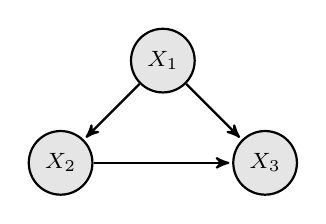
\begin{tikzpicture}[->,>=stealth',shorten >=1pt,auto,node distance=1cm,
  thick,main node/.style={observed}]

 %nodes
\node[main node](1){$X_{1}$};
\node[main node, below left=of 1](2){$X_{2}$};
\node[main node, below right=of 1](3){$X_{3}$};


 \path[every node/.style={font=\sffamily\small}]
    (1) edge node {} (2)
    	edge node {} (3)
    (2) edge node {} (3);
	
\end{tikzpicture}
\end{figure}



\begin{figure}
\centering
\caption{Some valid Bayesian networks for a distribution that an be factorised as $\P{X_1,X_2,X_3} = \P{X_1}\P{X_2|X_1}\P{X_3|X_2}$ (which implies $X_3 \ci X_1 | X_2$)}
\label{fig:bayesnet2}
\begin{subfigure}[t]{0.15\textwidth}
\centering
\caption{}
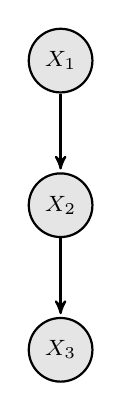
\begin{tikzpicture}[->,>=stealth',shorten >=1pt,auto,node distance=1cm, thick,main node/.style={observed}]
 %nodes
\node[main node](1){$X_{1}$};
\node[main node, below=of 1](2){$X_{2}$};
\node[main node, below=of 2](3){$X_{3}$};
\path[every node/.style={font=\sffamily\small}]
    (1) edge (2)
    (2) edge (3);
\end{tikzpicture}
\end{subfigure}
\begin{subfigure}[t]{0.15\textwidth}
\centering
\caption{}
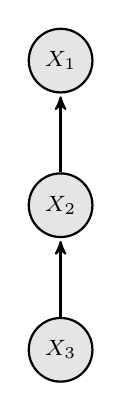
\begin{tikzpicture}[->,>=stealth',shorten >=1pt,auto,node distance=1cm, thick,main node/.style={observed}]
 %nodes
\node[main node](1){$X_{1}$};
\node[main node, below=of 1](2){$X_{2}$};
\node[main node, below=of 2](3){$X_{3}$};
\path[every node/.style={font=\sffamily\small}]
    (3) edge (2)
    (2) edge (1);
\end{tikzpicture}
\end{subfigure}
\begin{subfigure}[t]{0.3\textwidth}
\centering
\caption{}
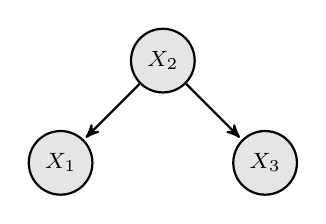
\begin{tikzpicture}[->,>=stealth',shorten >=1pt,auto,node distance=1cm, thick,main node/.style={observed}]
 %nodes
\node[main node](1){$X_{2}$};
\node[main node, below left=of 1](2){$X_{1}$};
\node[main node, below right=of 1](3){$X_{3}$};
\path[every node/.style={font=\sffamily\small}]
    (1) edge (2) edge (3);
\end{tikzpicture}
\end{subfigure}
\begin{subfigure}[t]{0.3\textwidth}
\centering
\caption{}
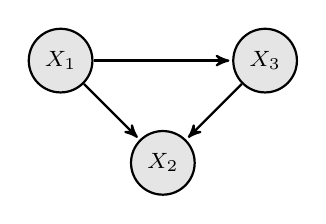
\begin{tikzpicture}[->,>=stealth',shorten >=1pt,auto,node distance=1cm, thick,main node/.style={observed}]
 %nodes
\node[main node](1){$X_{2}$};
\node[main node, above left=of 1](2){$X_{1}$};
\node[main node, above right=of 1](3){$X_{3}$};
\path[every node/.style={font=\sffamily\small}]
    (2) edge (1)
    (3) edge (1)
    (2) edge (3);
\end{tikzpicture}
\end{subfigure}
\end{figure}



The statement that a given graph $G$ is a Bayesian network for a distribution $P$ tells us that the distribution can be factorised over the nodes and edges in the graph. There can be no missing edges in $G$ that do not correspond to conditional independencies in $P$, (the converse is not true $G$ can have extra edges). If we let $parents_{X_{i}}$ represent the set of variables that are parents of the variable $X_{i}$ in $G$ then we can write the joint distribution as; 

\eqn{
\P{X_{1},...,X_{N}} = \prod_{i = 1...N}\P{X_{i}|parents_{X_{i}}}
}

A causal Bayesian network is a Bayesian network in which a link $X_{i} \rightarrow X_{j}$, by definition, implies $X_{i}$ causes $X_{j}$. This means that if we intervene and change the value of $X_{i}$, we expect $X_{j}$ to change, but if we intervene to change $X_{j}$, $X_{i}$ will not change. We need some notation to describe interventions and represent distributions over variables in the network after an intervention. In this thesis I use the do operator introduced by Pearl \citep{Pearl2000}.


\begin{definition}{The do-notation}
\begin{itemize}
\item $do(X=x)$ denotes an intervention that sets the random variable(s) $X$ to $x$.
\item $\P{Y|do(X)}$ is the distribution of $Y$ conditional on an \emph{intervention} that sets $X$. This notation is somewhat overloaded. It may be used represent a probability distribution/mass function or a family of distribution functions depending on whether the variables are discrete or continuous and whether or not we are treating them as fixed. For example it could represent 
\begin{itemize}
\item the probability $\P{Y=1|do(X=x)}$ as a function of $x$,
\item the probability mass function for a discrete $Y$ : $\P{Y|do(X=x)}$,
\item the probability density function for a continuous  $Y$ : $f_Y(y|do(X=x))$,
\item a family of density/mass function for $Y$ parameterised by $x$.
\end{itemize}
Where the distinction is important and not clear from context we will use one of the more specific forms above. 
\end{itemize}
\end{definition}


\begin{theorem}[Truncated product formula \citep{Pearl2000}]
\label{thm:truncated_prodcut}
If $G$ is a causal network for a distribution $P$ defined over variables $X_{1}...X_{N}$, then we can calculate the distribution after an intervention where we set $Z \subset X$ to $z$, denoted $do(Z=z)$ by dropping the terms for each of the variables in $Z$ from the factorisation given by the network. 

\begin{equation}
\label{eq:truncatedproduct}
\P{X_1...X_N|do(Z=z)} =
  \begin{cases}
  \prod_{i \notin Z}\P{X_{i}|parents_{X_{i}}} & \text{if $(X_{1}...X_{N})$ consistent with $Z=z$}  \\
   0       & \text{otherwise } 
  \end{cases}
\end{equation}
\end{theorem}


Theorem \ref{thm:truncated_prodcut} does not hold for standard Bayesian networks because there are multiple valid networks for the same distribution. The truncated product formula will give different results depending on the selected network. The result is possible with causal Bayesian networks because it follows directly from the assumption that the direction of the link indicates causality. In fact, from the interventionist viewpoint of causality, the truncation product formula defines what it means for a link to be causal. 


Returning to example \ref{exm:ranomized_experiment}, and phrasing our query in terms of interventions; what would the distribution of outcomes look like if everyone was treated $\P{Y|do(X=1)}$, relative to if no one was treated $\P{Y|do(X=0)}$? The treatment $X$ is a potential cause of $Y$, along with other unobserved variables, such as the age, gender and the disease sub-type of the patient. Since $X$ is assigned via deliberate randomisation we know that it is not affected by any latent variables. The causal Bayesian network for this scenario is shown in figure \ref{fig:causal_network_example}. This network represents the (causal) factorisation  $\P{X,Y} = \P{X}\P{Y|X}$, so from equation (\ref{eq:truncatedproduct}), $\P{Y|do(X)} = \P{Y|X}$. In this example, the interventional distribution is equivalent to the observational one.

\begin{figure}[h]
\caption{Causal Bayesian network for example \ref{exm:ranomized_experiment}}
\label{fig:causal_network_example}
\centering
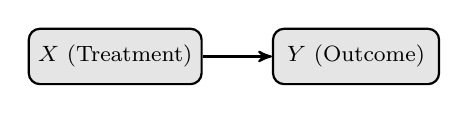
\begin{tikzpicture}[->,shorten >=0pt,shorten <=0pt,node distance=2.5em,thick,node/.style={observedrect},lt/.style={latent}]
\node[node](2){$X \text{ (Treatment)}$};
\node[node, right=of 2](3){$Y \text{ (Outcome)}$};
\path[]
	(2) edge (3);
\end{tikzpicture}
\end{figure}



In example \ref{exm:adjusting} we are interested in $\P{Y|do(X=1)}$, the expected high-school graduation rate if we introduce universal preschool. We could compare it to outlawing preschool $\P{Y|do(X=0)}$ or the current status quo $\P{Y}$. It seems reasonable to assume that preschool attendance affects the likelihood of high school graduation \footnote{The effect does not have to be homogeneous, it may depend non-linearly on characteristics of the child, family and school.} and that parental socio-economic status would affect \emph{both} the likelihood of preschool attendance and high school graduation. If we assume that socio-economic status is the only such variable (nothing else effects both attendance \emph{and} graduation), we can represent this problem with the causal Bayesian network in figure \ref{fig:causal_adjust}. In this case, the interventional distribution is not equivalent to the observational one. If parents with high socio-economic status are more likely to send their children to preschool and these children are more likely to graduate high school regardless, comparing the graduation rates of those who attended preschool with those who did not will overstate the benefit of preschool. To obtain the interventional distribution we have to estimate the impact of preschool on high school graduation for each socio-economic level separately and then weight the results by the proportion of the population in that group,

\eqn{
\label{eqn:backdoor_example}
\P{Y|do(X=1)} = \sum_{z \in Z}\P{Y|X=1,Z}\P{Z}
} 

We have seen from these two examples that the expression to estimate the causal effect of an intervention depends on the structure of the causal graph. There is a very powerful and general set of rules that specifies how we can transform observational distributions into interventional ones for a given graph structure. These rules are referred to as the Do-calculus \cite{Pearl2000}. We discuss them further in section \ref{sec:do_calculus}. 


\begin{figure}
\center
\caption{Causal Bayesian network for example \ref{exm:adjusting}}
\label{fig:causal_adjust}
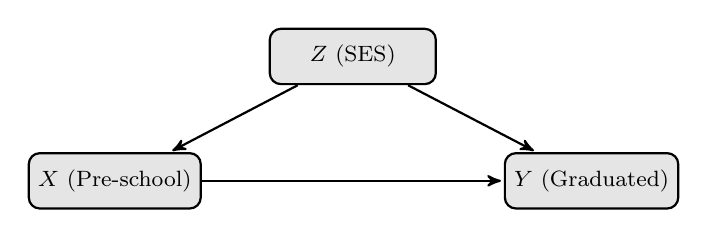
\begin{tikzpicture}[->,>=stealth',shorten >=1pt,auto,node distance=1.2cm, thick,node/.style={observedrect},lt/.style={latent}]

 %nodes
\node[node](1){$Z \text{ (SES)}$};
\node[node, below left=of 1](2){$X \text{ (Pre-school)}$};
\node[node, below right=of 1](3){$Y \text{ (Graduated)}$};
\path[every node/.style={font=\sffamily\small}]
    (1) edge (2) edge (3)
    (2) edge (3); 
\end{tikzpicture} 
\end{figure}

Formalising the definition of an intervention within the framework of causal graphical models provides us with an explicit mechanism to map information from one data generating process, the system pre-intervention, to another, the system post-intervention. The power of defining an intervention in this way stems from the number of things that are invariant between the two processes. All the (conditional) distributions for variables in the graph that were not directly set by the intervention are assumed not be changed by it.  

We could represent problems of the type where we try to infer properties of the post-interventional system based on data generated by the pre-interventional distribution by explicitly representing both systems and what they have in common, see figure \ref{fig:causal_ordinary_bayes}. This does not require any special framework or notation. The graphs in figure  \ref{fig:causal_ordinary_bayes} are ordinary Bayesian networks. However, without a causal framework, we have to make assumptions about what will be invariant to the intervention specifically for each such problem we encounter. For complex problems, it is very difficult to conceptualise the assumptions we expect to hold without the benefit of a causal framework.  


\begin{figure}[h]
\center
\caption{Causal inference with ordinary Bayesian networks. The plate on the left represents the observed data generated prior to the intervention and the plate on the right the data we anticipate obtaining after an intervention that sets the pre-interventional variable $X$ to $x$. The assumptions characterised by this plate model correspond to those implied by the causal Bayesian network in figure \ref{fig:causal_adjust} for the intervention $do(X=x)$. As the networks in this figure are ordinary Bayesian networks, we could have represented the same information with a different ordering of the links within each plate. However, we would then have a complex transformation relating the parameters between the two plates rather than a simple invariance.}
\label{fig:causal_ordinary_bayes}
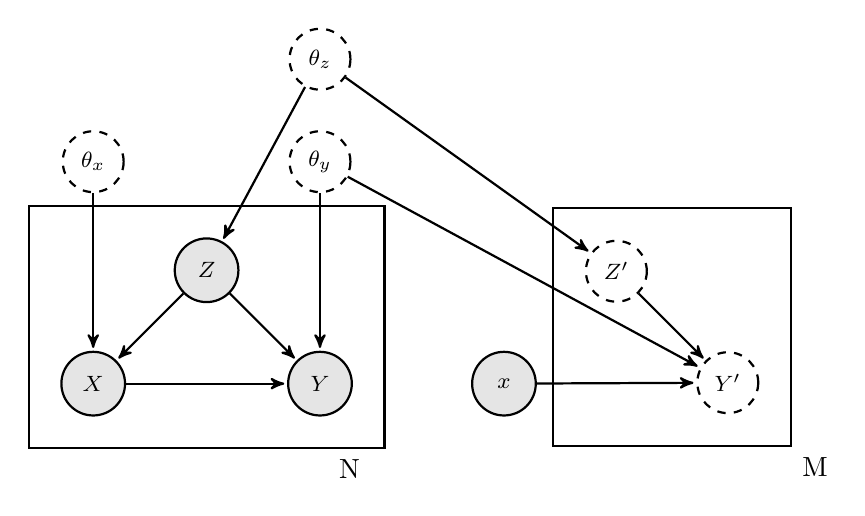
\begin{tikzpicture}[->,>=stealth',shorten >=1pt,auto,node distance=1.2cm, thick,node/.style={observed},lt/.style={latent}]
\tikzstyle{box}=[rectangle, draw=black!100]
 %nodes
\node[node](1){$Z$};
\node[node, below left=of 1](2){$X$};
\node[node, below right=of 1](3){$Y$};
\node[node, right=1.5cm of 3](4){$x$};
\node[lt, above right=of 4](5){$Z'$};
\node[lt, below right=of 5](6){$Y'$};
\node[lt, above=2.0cm of 3](9){$\theta_{y}$};
\node[lt, above=0.5cm of 9](7){$\theta_z$};
\node[lt, above=2.0cm of 2](8){$\theta_x$};
\path[every node/.style={font=\sffamily\small}]
    (1) edge (2) edge (3)
    (2) edge (3)
    (4) edge (6)
    (5) edge (6)
    (8) edge (2)
    (7) edge (1) edge (5)
    (9) edge (3) edge (6);
\node[rectangle, inner sep=4.0mm, fit= (1) (2) (3),draw=black!100,label=below right:N] {};
\node[rectangle, inner sep=4.0mm, fit= (5) (6),draw=black!100,label=below right:M] {};
\end{tikzpicture} 
\end{figure}

A causal Bayesian network represents much more information than a Bayesian network with identical structure. A causal network encodes all possible interventions that could be specified with the do-notation. For example, if the network in figure \ref{fig:causal_adjust} were an ordinary Bayesian network and all the variables were binary, the associated distribution could be described by 7 parameters. The equivalent causal Bayesian network additionally represents the post-interventional distributions for six possible single variable interventions and twelve possible two variable interventions. Encoding all this information without the assumptions implicit in the causal Bayesian network would require an additional 30 parameters \footnote{After each single variable intervention we have a distribution over two variables, which can be represented by three parameters. After each two variable intervention, we have a distribution over one variables which requires one parameter. This takes us to a total of $6\times3+12\times1 = 30$ additional parameters.}.


Causal Bayesian networks are Bayesian networks, so results that apply to Bayesian networks carry directly across; the local Markov property states that variables are independent of their non-effects given their direct causes. Similarly the global Markov property and d-separation also hold in causal networks. 

\subsubsection{Limitations of causal Bayesian networks}
A number of criticisms have been levelled at this approach to modelling causality. One is that the definition of an intervention only in terms of setting the value of one or more variables is too precise and that any real world intervention will affect many variables in complex and non-deterministic ways \citep{rickles2009causality,cartwright2007hunting}. However, by augmenting the causal graph with additional variables that model how interventions may take effect, the deterministic do operator can model more complex interventions. For example, in the drug treatment case, we assumed that all subjects complied, taking the treatment or placebo as assigned by the experimenter. But what if some people failed to take the prescribed treatment. We can model this within the framework of deterministic interventions by adding a node representing what they were prescribed (the intervention) which probabilistically influences the treatment they actually receive, see figure \ref{fig:randomized_imperfect_compliance}. Note that the fact that we no longer directly assign the treatment opens the possibility that an unobserved latent variable could affect both the actual treatment taken and the outcome.

\begin{figure}[h]
\caption{Randomised treatment with imperfect compliance}
\label{fig:randomized_imperfect_compliance}
\centering
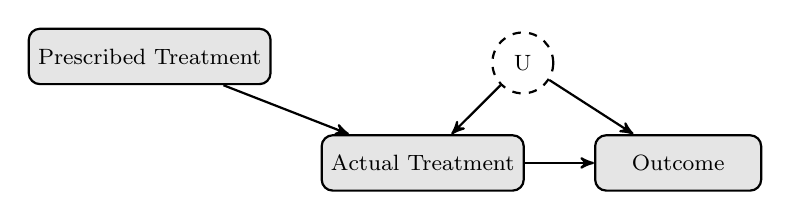
\begin{tikzpicture}[->,shorten >=0pt,shorten <=0pt,node distance=2.5em,thick,node/.style={observedrect},lt/.style={latent}]
\node[node](1){Prescribed Treatment};
\node[node, below right=of 1](2){Actual Treatment};
\node[node, right=of 2](3){Outcome};
\node[lt, above left=of 3](4){U};
\path[]
	(1) edge (2)
	(2) edge (3) 
	(4) edge (3) edge (2);
\end{tikzpicture}
\end{figure}

Another key issue with causal Bayesian networks is that they cannot handle cyclic dependencies between variables. Such feedback loops are common in real-life systems, for example the relationship between supply and demand in economics or predator and prey in ecology. We might regard the underlying causal mechanisms in these examples to be acyclic; the number of predators at one time influences the number of prey in the next period and so on. However, if our measurements of these variables must be aggregated over time frames that are longer than the scale at which these interactions occur the result is a cyclical dependency. Even were we able to measure on shorter timescales, we might then not have sufficient data on each variable for inference. Such problems have mostly been studied within the dynamic systems literature, typically focusing on understanding the stationary or equilibrium state of the system and making very specific assumptions about functional form in order to make problems tractable. \citet{Poole2013} compare the equilibrium approach to reasoning about cyclic problems with structural equation models, which we discuss in section \ref{sec:SEM} and which can be seen as Bayesian causal networks with additional functional assumptions. 

\section{Counterfactuals}
\label{sec:counterfactuals}

The Neyman-Rubin model \citep{Rubin1974,Rubin1978,Rosenbaum1983, Rubin2005,Rubin2008} defines causality in terms of potential outcomes, or counterfactuals. Counterfactuals are statements about imagined or alternate realities, are prevalent in everyday language and may play a role in the development of causal reasoning in humans \citep{Weisberg2013}. Causal effects are differences in counterfactual variables: what is the difference between what would have happened if we did one thing versus what would have happened if we did something else. 

In example \ref{exm:ranomized_experiment}, the causal effect of the drug relative to placebo for person $i$ is the difference between what would have happened if they were given the drug, denoted $\cf{y_{i}}{1}$ versus what would have happened if they got the placebo, $\cf{y_{i}}{0}$. The fundamental problem of causal inference is that we can only observe one of these two outcomes, since a given person can only be treated or not treated. The problem can be resolved if, instead of people, there are units that can be assumed to be identical or that will revert exactly to their initial state some time after treatment. This type of assumption often holds to a good approximation in the natural sciences and explains why researchers in these fields are less concerned with causal theory. 

Putting aside any estimates of individual causal effects, it is possible to learn something about the distributions under treatment or placebo. Let $\cf{Y}{1}$ be a random variable representing the potential outcome if treated. The distribution of $\cf{Y}{1}$ is the distribution of $Y$ if everyone was treated. Similarly $Y^{0}$ represents the potential outcome for the placebo. The difference between the probability of recovery, across the population, if everyone was treated and the probability of recovery given placebo is $\P{\cf{Y}{1}}-\P{\cf{Y}{0}}$. We can estimate (from an experimental or observational study):
\begin{itemize}
\item $\P{Y|X=1}$, the probability that those who took the treatment will recover
\item $\P{Y|X=0}$, the probability that those who were not treated will recover
\end{itemize}

Now, for those who took the treatment, the outcome \emph{had} they taken the treatment $\cf{Y}{1}$ is the same as the observed outcome. For those who did not take the treatment, the observed outcome is the sames as the outcome \emph{had} they not taken the treatment. Equivalently stated:

\eq{
\P{Y^{0}|X=0}&= \P{Y|X=0}\\
\P{Y^{1}|X=1}&=\P{Y|X=1}
}

If we assume $X \ci Y^{0}$ and $X \ci Y^{1}$:

\eq{
\P{Y^{1}} &= \P{Y^{1}|X=1} = \P{Y|X=1} \\
\P{Y^{0}} &= \P{Y^{0}|X=0} = \P{Y|X=0}
}

This implies the counterfactual distributions are equivelent to the corresponding conditional distributions and, for a binary outcome $Y$, the causal effect is,

\eq{
\P{Y^{1}}-\P{Y^{0}} = \P{Y|X=1} - \P{Y|X=0}
}

The assumptions $X \ci Y^{1}$ and $X \ci Y^{0}$  are referred to as ignorebility assumptions \citep{Rosenbaum1983}. They state that the treatment each person receives is independent of whether they would recover if treated and if they would recover if not treated. This is justified in example \ref{exm:ranomized_experiment} due to the randomisation of treatment assignment. In general the treatment assignment will not be independent of the potential outcomes. In example \ref{exm:adjusting}, the children who attended preschool may be more likely to have graduated high school had they in fact not attended than the children who actually did not attend, $X \nci \cf{Y}{0}$. Similarly, had the poorer children who did not attend pre-school attended they might not have done as well as the children who did in fact attend, $X \nci \cf{Y}{1}$. A more general form of the ignorebility assumption is to identify a set of variables $Z$ such that $X \ci Y^{1}|Z$ and $X \ci Y^{0}|Z$. 

\vspace*{.3cm}
\begin{theorem}[Ignorability] If $X \ci Y^{1}|Z$ and $X \ci Y^{0}|Z$,

\eqn{
\label{eqn:counterfactual1}
\P{\cf{Y}{1}} &= \sum_{z \in Z}\P{Y|X=1,Z}\P{Z}  \\
\label{eqn:counterfactual2}
\P{\cf{Y}{0}} &= \sum_{z \in Z}\P{Y|X=0,Z}\P{Z}
}
\end{theorem}

Assuming that within each socio-economic status level, attendance at pre-school is independent of the likelihood of graduating high-school had a person attended, then the average rate of high-school graduation given a universal pre-school program can be computed from equation \ref{eqn:counterfactual1}. Note, that this agrees with the weighted adjustment formula in equation \ref{eqn:backdoor_example}. 

Another assumption introduced within the Neyman-Rubin causal framework is the Stable Unit Treatment Value Assumption (SUTVA) \citep{Rubin1978}. This is the assumption that the potential outcome for one individual (or unit) does not depend on the treatment assigned to another individual. As an example of a SUTVA violation, suppose disadvantaged four year olds were randomly assigned to attend pre-school. The subsequent school results of children in the control group, who did not attend, could be boosted by the improved behaviour of those who did and who now share the classroom with them. SUTVA violations would manifest as a form of model misspecification in causal Bayesian networks. 


There are complex philosophical objections to counterfactuals arising from the way they describe alternate universes that were never realised. This makes it quite easy to (accidentally) make statements about counterfactuals that cannot be tested with empirical data. Consider the following example based on \citet{Dawid2000}. Again we have a drug where the outcome for an individual if treated is represented by the counterfactual variable $\cf{Y}{1}$ and the outcome if not treated is $\cf{Y}{0}$. Suppose these counterfactual variables $\cf{Y}{1}$ and $\cf{Y}{0}$ are jointly normal with equal variance (for simplicity).

% vector with mean mu_t,mu_c and a covariance matrix
\eqn{
P(\cf{Y}{1},\cf{Y}{0}) \sim N( 
         \begin{bmatrix}
           \mu_{1} \\
           \mu_2 \\
         \end{bmatrix},
         \begin{bmatrix}
           \sigma^2 & \rho \sigma^2 \\
           \rho \sigma^2 & \sigma^2 \\
         \end{bmatrix}
         )
}

Their difference is also normal. Let $\tau = \cf{Y}{1} - \cf{Y}{0}$,

\eqn{
P(\tau) = N(\mu_1 - \mu_0,2\sigma^{2}(1-\rho))
}


\begin{figure}[h]
\captionsetup[subfigure]{position=b}
\centering
\caption{The distribution of individual treatment effects is not identifiable, even from a randomised controlled trial.}
\label{fig:metaphysical_distribution_difference}
\subcaptionbox{Marginal distributions over the potential outcomes $\cf{Y}{1}$ and $\cf{Y}{0}$ for $\mu_1=1$, $\mu_0=0$ and $\sigma = 1$. The blue curve shows the distribution of $Y$ if everyone were to be treated and the blue curve the distribution if no-one was treated. \label{fig:metaphys_a}}{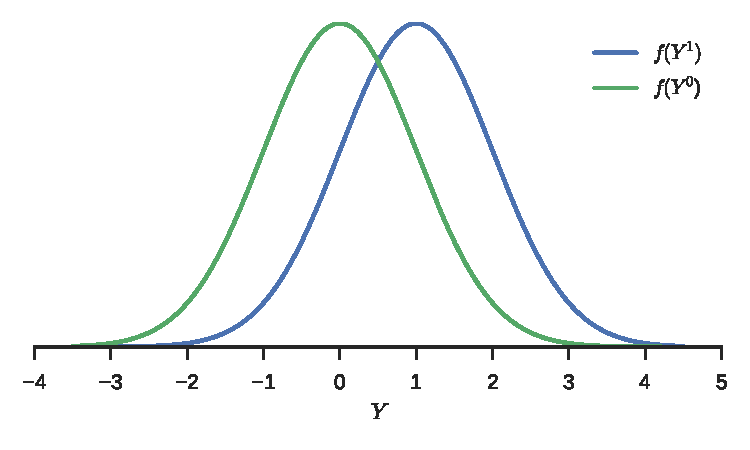
\includegraphics[width=.45\linewidth]{figures/counterfactual_nonidentify_a.pdf}}
\hspace{0.02\textwidth}
\subcaptionbox{Two very different distributions of individual causal effects consistent with the potential outcome distributions. \label{fig:metaphys_b}}
{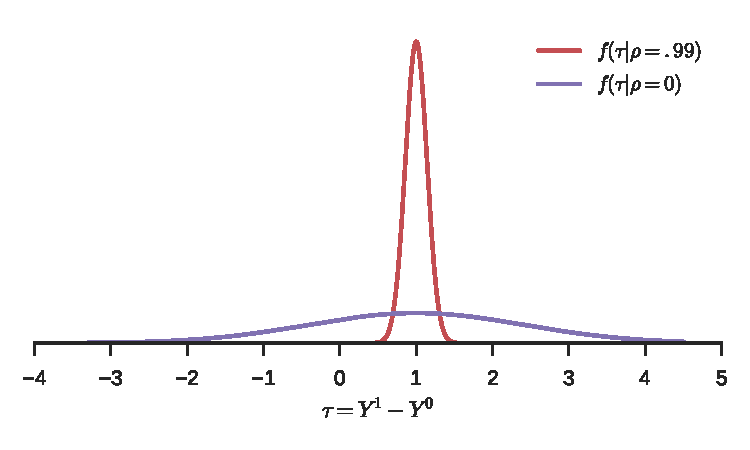
\includegraphics[width=.45\linewidth]{figures/counterfactual_nonidentify_b.pdf}}
\end{figure}

From a (large) randomised controlled trial we can estimate the marginal distributions over the counterfactual variables, see figure \ref{fig:metaphys_a}. These represent the distributions we would expect over the outcome $Y$ if everyone were treated or not treated respectively. However, the distribution over the individual causal effects depends on $\rho$, see figure \ref{fig:metaphys_b}. The key problem is that we can never observe the joint distribution over $\cf{Y}{1}$ and $\cf{Y}{0}$. As a result, $\rho$ and thus the variance of $\tau$ is not identifiable, even from experimental data. \citet{Dawid} argues that we should avoid using counterfactuals as they are defined in terms of (metaphysical) individual causal effects. He further points out that the interventional distributions in figure \ref{fig:metaphys_a}, along with a loss function, contain all the information required to decide how to treat a new patient.  

This result is unintuitive. It seems on the face of it that the distribution of individual causal effects is relevant to our decision making. If $\rho = 1$ then almost everyone benefits slightly from the treatment whilst if $\rho=0$, there is a wide range, with some people benefiting a lot and others suffering significant harm. This confusion can be resolved by thinking about personalised rather than individual causal effects. It is entirely possible that potentially observable characteristics (such as gender, age, genetics, etc) affect how people will respond to the treatment. We can partition people into sub-populations on the basis of these characteristics and measure different \emph{personalised} causal effects for each group. The variance of the potential outcome distributions $f(\cf{Y}{1})$ and $f(\cf{Y}{0})$ provides bounds on how much can be gained from further personalisation. The metaphysical nature of individual causal effects only arises when we are at the point where the only remaining variation is due to inherent randomness (or variables that we could not even in principle measure). 

One way of looking at counterfactuals is as a natural language short hand for describing highly specific interventions like those denoted by the do-notation. Rather than talking about the distribution of $Y$ given we intervene to set $X=x$ and hold everything else about the system constant we just say what would the distribution of $Y$ be had $X$ been $x$. This is certainly convenient, if rather imprecise. However, the ease with which we can make statements with counterfactuals that cannot be tested with empirical data warrants careful attention. It is important to be clear what assumptions are being made and whether or not they could be validated (at least in theory). 

\section{Structural Equation models}
\label{sec:SEM}

Structural equation models (SEMs) describe a deterministic world, where some underlying mechanism or function determines the output of any process for a given input. The mechanism (but not the output) is assumed to be independent of what is fed into it. Uncertainties are not inherent but arise from unmeasured variables. Linear structural equation models have a long history for causal estimation \cite {Wright1921,Haavelmo1943}. More recently, they have been formalised, generalised to the non-linear setting and connected to developments in graphical models to provide a powerful causal framework \citep{Pearl2000}.

Mathematically, each variable is a deterministic function of its direct causes and a noise term that captures unmeasured variables. The noise terms are required to be mutually independent. If there is the possibility that an unmeasured variable influences more than one variable of interest in a study, it must be modelled explicitly as a latent variable. Structural equation models can be represented visually as a network. Each variable is a node and arrows are drawn from causes to their effects. Figure \ref{fig:sem_randomized_treatment} illustrates the SEM for example \ref{exm:ranomized_experiment}.

\begin{figure}[h]
\caption{SEM for example \ref{exm:ranomized_experiment}}
\label{fig:sem_randomized_treatment}
\centering
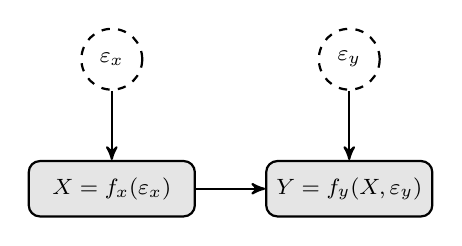
\begin{tikzpicture}[->,shorten >=0pt,shorten <=0pt,node distance=2.5em,thick,node/.style={observedrect},lt/.style={latent}]
\node[node](2){$X = f_x(\epsilon_x)$};
\node[node, right=of 2](3){$Y = f_y(X,\epsilon_y)$};
\node[lt, above=of 3](4){$\epsilon_y$};
\node[lt, above=of 2](5){$\epsilon_x$};
\path[]
	(2) edge (3)
	(4) edge (3)
	(5) edge (2);
\end{tikzpicture}
\end{figure}

This model encodes the assumption that the outcome $y_{i}$ for an individual $i$ is caused solely by the treatment $x_{i}$ they receive and other factors $\epsilon_{y_{i}}$ that are independent of $X$. This is justifiable on the grounds that $X$ is random. The outcome of a coin flip for each patient should not be related to any of their characteristics (hidden or otherwise). Note that the causal graph in figure \ref{fig:sem_randomized_treatment} is identical to that the Bayesian network for the same problem, figure \ref{fig:causal_network_example}. The latent variables $\epsilon_x$ and $\epsilon_y$ are not explicitly drawn in figure \ref{fig:causal_network_example} as they are captured by the probabilistic nature of the nodes in a Bayesian network.

Taking the \emph{action} $X=1$ corresponds to replacing the equation $X=f_x(\epsilon_x)$ with $X=1$. The function $f_y$ and distribution over $\epsilon_y$ does not change. This results in the interventional distribution \footnote{We have assumed the variables are discrete only for notational convenience},

\eqn {
\P{Y=y|do(X=1)} = \sum_{\epsilon_y}\P{\epsilon_y}\ind{f_y(1,\epsilon_y)=y}
}

The observational distribution of $Y$ given $X$ is,

\eqn{
\P{Y=y|X=1} &= \sum_{\epsilon_x}\sum_{\epsilon_y}\P{\epsilon_x|X=1}\P{\epsilon_y|\epsilon_x}\ind{f_y(1,\epsilon_y)=y} \\
& = \sum_{\epsilon_y}\P{\epsilon_y}\ind{f_y(1,\epsilon_y)=y} \text{, as } \epsilon_x \ci \epsilon_y
}

The interventional distribution is the same as the observational one. The same argument applies to the intervention $do(X=0)$ and so the causal effect is simply the difference in observed outcomes as found via the causal Bayesian network and counterfactual approaches. 

The SEM for example \ref{exm:adjusting} is shown in figure \ref{fig:sem:preschool}. Intervening to send all children to pre-school replaces the equation $X = f_x(Z,\epsilon_x)$ with $X=1$, leaving all the other functions and distributions in the model unchanged. 

\eqn{
\P{Y=y|do(X=1)} &= \sum_{z}\sum_{\epsilon_y}\P{z}\P{\epsilon_y}\ind{f_y(1,z,\epsilon_y)=y} \\
\label{eqn:sem:adjusting}
&=\sum_{z}\P{z}\underbrace{\sum_{\epsilon_y}\P{\epsilon_y}\ind{f_y(1,z,\epsilon_y)=y}}_{\P{Y=y|X=1,Z=z}}
}
Equation \ref{eqn:sem:adjusting} corresponds to equations \ref{eqn:backdoor_example} and \ref{eqn:counterfactual1}. It is not equivalent to the observational distribution given by:

\eqn{
\P{Y=y|X=1} = \sum_{z}\sum_{\epsilon_y}\P{z|X=1}\P{\epsilon_y}\ind{f_y(1,z,\epsilon_y)=y}
}


\begin{figure}[h]
\caption{SEM for example \ref{exm:adjusting}}
\label{fig:sem:preschool}
\centering
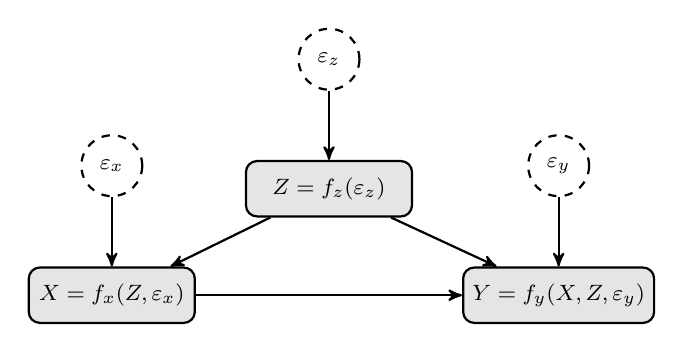
\begin{tikzpicture}[->,shorten >=0pt,shorten <=0pt,node distance=2.5em,thick,node/.style={observedrect},lt/.style={latent}]
\node[node](2){$X = f_x(Z,\epsilon_x)$};
\node[node,above right=of 2](6){$Z = f_z(\epsilon_z)$};
\node[lt, above=of 6](7){$\epsilon_z$};
\node[node, below right=of 6](3){$Y = f_y(X,Z,\epsilon_y)$};
\node[lt, above=of 3](4){$\epsilon_y$};
\node[lt, above=of 2](5){$\epsilon_x$};
\path[]
	(2) edge (3)
	(4) edge (3)
	(5) edge (2)
	(7) edge (6)
	(6) edge (2) edge (3);
\end{tikzpicture}
\end{figure}

Structural equation models are generally applied with strong constraints on the functional form of the relationship between the variables and noise is typically assumed to be additive, $X_i = f_i(\cdot)+\epsilon_i$. A structural equation model with $N$ variables resembles a set of $N$ simultaneous equations, with each variable playing the role of the dependent (left hand side) variable in one equation. However a SEM is, by definition, more than a set of simultaneous equations. By declaring it to be structural we are saying that it represents assumptions about the relationships between variables. When we visualise the model as a network the absence of an arrow between two variables encodes the assumption that one does not cause the other. The similarity between the notation used to describe and analyse structural equation models and simultaneous equations, combined with a reluctance to make explicit statements about causality, has led to some confusion in the interpretation of SEMs \citep{heckman2015causal,Pearl2000}. 

\section{Comparing and unifying the models}

Remarkably for models developed relatively independently in fields with very different approaches and problems, the models we have discussed can be nicely unified for interventional queries (those that can be expressed with the do-notation). If the network for a structural equation model is acyclic, that is if starting from any node and following edges in the direction of the arrows you cannot return to the starting point, then it implies a recursive factorisation of the joint distribution over its variables. In other words, the network is a causal Bayesian network. All of the results that apply to causal Bayesian networks also apply to acyclic structural equation models.  Taking an action that sets a variable to a specific value equates to replacing the equation for that variable with a constant. This corresponds to dropping a term in the factorisation and the truncated product formula (equation \ref{eq:truncatedproduct}). Thus, the interventional query $P(Y|do(X))$ is identical in these two frameworks. We can also connect this to counterfactuals via:

\begin{equation}
\begin{aligned}
&Y^{0} \equiv P(Y|do(X=0)) \\
&Y^{1} \equiv P(Y|do(X=1))
\end{aligned}
\end{equation}

The assumption $\epsilon_{X} \ci \epsilon_{Y}$, stated for our structural equation model, translates to $X \ci (Y^{0},Y^{1})$ in the language of counterfactuals. When discussing the counterfactual model, we actually made the slightly weaker assumption:

\begin{equation}
\label{eq:weakignore}
X \ci Y^{0} \text{ and } X \ci Y^{1}
\end{equation}

It is possible to relax the independence of errors assumption for SEMs to correspond exactly with the form of equation (\ref{eq:weakignore}) without losing any of the power provided by d-separation and graphical identification rules \citep{Richardson2013}. The correspondence between the models for interventional queries (those that can be phrased using the do-notation) makes it straightforward to combine key results and algorithms developed within any of these frameworks. For example, you can draw a causal graphical network to determine if a problem is identifiable and which variables should be adjusted for to obtain an unbiased causal estimate. Then use propensity scores \citep{Rosenbaum1983} to estimate the effect. If non-parametric assumptions are insufficient for identification or lead to overly large uncertainties, you can specify additional assumptions by phrasing your model in terms of structural equations. The frameworks do differ when it comes to causal queries that involve joint or nested counterfactuals and cannot be expressed with the do-notation. These types of queries arise in the study of mediation \citep{Pearl2014,Imai2010a,VanderWeele2011} and in legal decisions, particularly on issues such as discrimination \citep{Pearl2000}. 

In practice, differences in focus and approach between the fields in which each model dominates eclipse the actual differences in the frameworks. The work on causal graphical models \citep{Pearl2000,Sprites} focuses on asymptotic, non-parametric estimation and rigorous theoretical foundations. The Neyman-Rubin framework builds on the understanding of randomised experiment and generalises to quasi-experimental and observational settings, with a particular focus on non-random assignment to treatment. This research emphasises estimation of average causal effects and provides practical methods for estimation, in particular, propensity scores; a method to control for multiple variables in high dimensional settings with finite data \citep{Rosenbaum1983}. In economics, inferring causal effects from non-experimental data to support policy decisions is central to the field. Economists are often interested in more informative measures of the distribution of causal effects than the mean and make extensive use of structural equation models, generally with strong parametric assumptions \citep{Heckman2008}. In addition, the parametric structural equation models favoured in economics can be extended to analyse cyclic (otherwise referred to as non-recursive) models. 

\section{What does a causal model give us? Resolving Simpson's paradox}

We will now demonstrate our new notation and frameworks for causal inference to resolve a fascinating paradox, noted by \citet{yule1903notes}, demonstrated in real data by \citet{Cohen1934} and popularised by \citet{simpson1951interpretation}. The following example is adapted from \citet{Pearl2000}. Suppose a doctor has two treatments, A and B, which she offers to patients to prevent heart disease. She keeps track of which medication her patients choose and whether or not the treatment is successful. She obtains the results in table \ref{tab:simpson1}.

\begin{table}[h]
\caption{Treatment results}
\label{tab:simpson1}
\center
\begin{tabular}{c c c c c}
Treatment & Success & Fail & Total & Success Rate\\
\hline
\rowcolor[gray]{0.9} 
A &  87 & 13 & 100 & 87\%\\
\rowcolor{white} B & 75 & 25 & 100 & 75\%\\
\hline
\end{tabular}
\end{table}

Drug A appears to perform better. However, having read the latest literature on how medications affect men and women differently, she decides to break down her results by gender to see how well the drugs perform for each group and obtains the data in table \ref{tab:simpson2}.

\begin{table}[h]
\caption{Treatment results by gender}
\label{tab:simpson2}
\center
\begin{tabular}{c c c c c c}
Gender & Treatment & Success & Fail & Total & Success Rate\\
\hline
\rowcolor[gray]{0.9}
M & A & 12 & 8 & 20 & 60\%\\
M & B & 56 & 24 & 80 & 70\%\\
\rowcolor[gray]{0.9}
F & A & 75 & 5 & 80 & 94\%\\
F & B & 19 & 1 & 20 & 95\%\\
\hline
\end{tabular}
\end{table}

Once the data is broken down by gender, drug B looks better for both men \emph{and} women. Suppose the doctor must choose only one drug to prescribe to all her patients in future (perhaps she must recommend which to subsidise under a national health scheme). Should she choose A or B? The ambiguity in this question lies at the heart of Simpson's paradox. How does causal modelling resolve the paradox? The key is that the doctor is trying to choose between \emph{interventions}. She wants to know what the success rate will be if she changes her practice to give all the patients one drug, rather than allowing them to choose as currently occurs. 

Let's represent the treatment by the variable $T$, the gender of the patient by $Z$ and whether or not the treatment was successful by $Y$. The doctor cares about $\P{Y|do(T)}$, not the standard conditional distributions $\P{Y|T}$. Unfortunately, the data in tables \ref{tab:simpson1} and \ref{tab:simpson2} is insufficient to enable estimation of the interventional distribution $\P{Y|do(T)}$ or determine if $do(T=A)$ is better or worse than $do(T=B)$. Some assumptions about the causal relationships between the variables are required. In this example, it seems reasonable to conclude that gender may affect the treatment chosen and the outcome. Assuming there are no other such confounding variables (for example income) then we obtain the causal network in figure \ref{fig:simpsons_paradox}.

\begin{figure}[h]
\caption{An example of Simpson's Paradox}
\label{fig:simpsons_paradox}
\centering
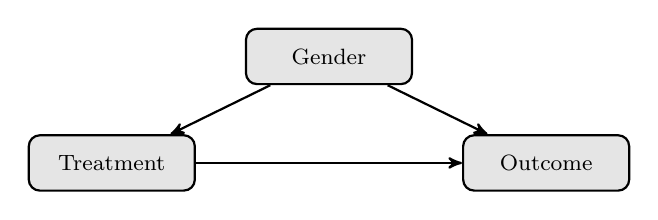
\begin{tikzpicture}[->,shorten >=0pt,shorten <=0pt,node distance=2.5em,thick,node/.style={observedrect},lt/.style={latent}]
\node[node](1){Gender};
\node[node, below left=of 1](2){Treatment};
\node[node, below right=of 1](3){Outcome};
\path[]
	(1) edge (2) edge (3) 
	(2) edge (3);
\end{tikzpicture}
\end{figure}

With this model, women are more likely to choose drug A and are also more likely to recover than men regardless of the treatment they receive. Knowing a patient took drug A indicates they are more likely to be female. When we compare the group of people who took A against those who took B, the effect of the higher proportion of females in the first group conceals the greater benefit of drug B leading to an apparent reversal in effectiveness. However, when the doctor intervenes to set the treatment each person receives there will no longer be a link from gender to treatment. So in this case she should choose which drug to prescribe from the gender specific table (and weight by the proportion of the population that belongs to each gender). Drug B is the better choice. 

\eqn{
\P{Y|do(T)} = \P{Y|T,female}\P{female}+ \P{Y|T,male}\P{male}
}

Is the solution to Simpson's paradox to always to break down the data by as many variables as possible? No. Suppose we have the identical data as in \ref{tab:simpson1} and \ref{tab:simpson2} but replace the column name 'gender' with 'blood pressure', 'M' with 'high' and 'F' with 'normal'. This is a drug designed to prevent heart disease. One pathway to doing so might well be to lower blood pressure. Figure \ref{fig:simpsons_paradox2} shows a plausible causal graph for this setting. It differs from the graph in figure \ref{fig:simpsons_paradox} only in the direction of a single link. Now, however, table \ref{tab:simpson2} tells us that people who took treatment $A$ had better blood pressure control and better overall outcomes. In this setting $\P{Y|do(T)} = \P{Y|T}$ and drug A is the better choice. 

\begin{figure}[h]
\caption{An example of Simpson's Paradox}
\label{fig:simpsons_paradox2}
\centering
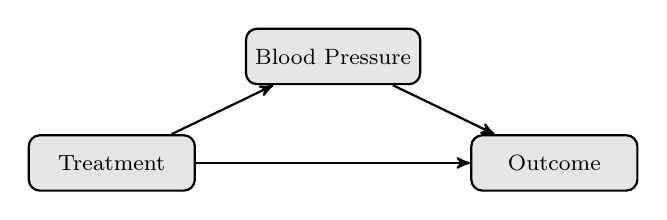
\begin{tikzpicture}[->,shorten >=0pt,shorten <=0pt,node distance=2.5em,thick,node/.style={observedrect},lt/.style={latent}]
\node[node](1){Blood Pressure};
\node[node, below left=of 1](2){Treatment};
\node[node, below right=of 1](3){Outcome};
\path[]
	(1) edge (3) 
	(2) edge (3)
	(2) edge (1);
\end{tikzpicture}
\end{figure}

Note that we have not changed the data itself, only the description of the variables that it is associated with. This illustrates that the resolution to Simpson's paradox lies fundamentally not in the data, but in the assumptions we are willing to make. From a purely statistical viewpoint there is no paradox. The reversal just stems from the mathematical property of ratios expressed in equation \ref{eqn:simpsons_paradox} and represented graphically in figure \ref{fig:simpsons_vector}. The paradox only arises when we attempt to use the data to select an intervention and is resolved when we apply a causal approach to do so.

\eqn{
\label{eqn:simpsons_paradox}
\exists \set{N_1,...N_4, N_1'...N_4'} \in \mathbb{N} : \; 
\textcolor{green}{\frac{N_1}{N_2}< \frac{N_1'}{N_2'}}, \;\; 
\textcolor{blue}{ \frac{N_3}{N_4}<\frac{N_3'}{N_4'}}
 \text{ and } \frac{N_1+N_3}{N_2+N_4} > \frac{N_1'+N_3'}{N_2'+N_4'}
}

\begin{figure}
\centering
\caption{Simpson's reversal visualised. The ratios involving $N_i'$ are steeper than than those involving $N_i$ for both the blue and green vectors. However, when we sum them, the ratio is steeper for the un-primed variables.}
\label{fig:simpsons_vector}
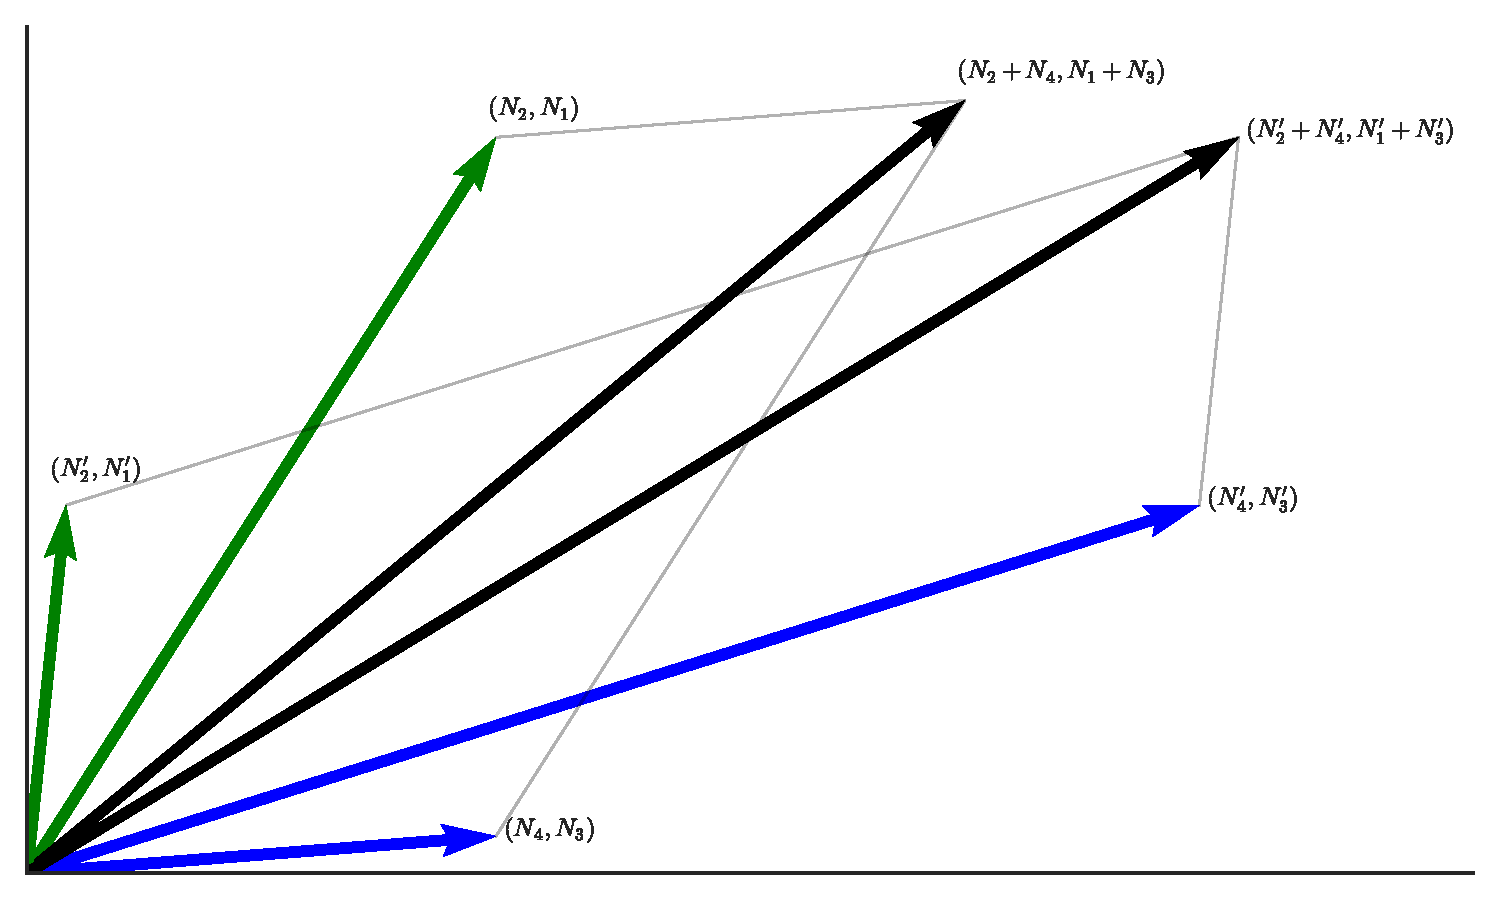
\includegraphics[scale=.4]{figures/simpson_vector}
\end{figure}

There are many other plausible causal graphs for both scenarios above. Perhaps income affects drug choice as well as gender, or gender might affect treatment choice and blood pressure control given treatment, etc. Causal modelling provides a powerful tool to specify such assumptions and to determine how to estimate causal effects for a given model see section \ref{sec:causal effect estimation}.

\chapter{Two key questions}
\label{chap:two_key_questions}

We can roughly categorise the problems studied within causal inference into two groups, causal effect estimation and causal discovery. In causal effect estimation we assume (at least implicitly) that key aspects of the causal graph are known. The goal is then to estimate the effect of an intervention or range of interventions in the system. Causal effect estimation is implicit in countless studies in economics, social science and epidemiology of everything from the effect of education on earnings \citep{card1999causal}, diet on cancer \citep{bingham2004diet} and breastfeeding on intelligence \citep{jain2002good} to the effect of pet ownership on survival after a heart attack \citep{friedmann1995pet}. Almost every time someone runs a regression model the key quantity of interest is a causal effect. Given how it underlies so much of our scientific progress, there is a enormous potential in properly understanding when we can draw causal conclusions, exactly what assumptions are required to do so and how we can best leverage those assumptions to infer as much information as we can from our data. 

Causal discovery aims to leverage much broader assumptions to learn the structure of causal graphs from data. This is critical in fields where we are generating a lot of data but have limited theoretical knowledge from which to draw on to determine how variables are related to one another. Causal discovery algorithms are being applied in bioinformatics \citep{Bay2002,Sachs2005,Ram2006,Alekseyenko2011,Statnikov2012,Gao2015,Sokolova2015,Taruttis2015}, medical imaging \citep{Ramsey2010} and climate science \citep{Uphoff2013}. An effective and generalisable approach for causal discovery would be a major step towards the automation of the scientific endeavour.

\section{Causal effect estimation} 
\label{sec:causal effect estimation}

Estimating causal effects from observational data comes down to determining if and how we can write expressions for the interventional distributions of interest in terms of observational quantities, which can be measured. We did this on an ad-hoc basis to resolve the examples discussed in chapter \ref{chap:causal_models}. In this chapter we describe a principled approach to mapping observational quantities to interventional ones and discuss some of the key issues involved in estimating such expressions from finite sample data. We assume the basic structure of the graph is known. That is, we assume that we can draw a network containing (at a minimum):

\begin{itemize}
\item the target/outcome variable we care about,
\item the focus/treatment variables on which we are considering interventions,
\item any variables which act to confound two or more of the other variables we have included, and
\item any links between variables we have included. 
\end{itemize}

Some of these variables may be latent in that the available data does not record their value, however their position in the network is assumed to be known. For example, consider estimating the impact of schooling on wages. Some measure of inherent ability could influence both the number of years of schooling people choose to pursue and the wages they receive. Even if we have no data to directly assess people's inherent ability we must include it in the graph because it influences two of the variables we are modelling. 

How can the structure of the causal graph be leveraged to compute interventional distributions from observational ones? Given the graph corresponding to the observational distribution, the graph after any intervention can be obtained by removing any links into variables directly set by the intervention. The joint interventional distribution is the product of the factors associated with the interventional graph, as given by the truncated product formula \ref{eq:truncatedproduct}. If there are no latent variables the interventional distribution of interest can be obtained by marginalising over the joint (interventional) distribution. However, if there are latent variables the joint interventional distribution will contain terms that cannot be estimated from the observed data. 

The key to estimating causal effects in the presence of latent variables lies in combining the assumption of how an intervention changes the graph, encoded by the truncated product formula, with information the graph structure provides about conditional independencies between variables. 
By leveraging conditional independencies we can effectively localise the effect of an intervention to a specific part of a larger graph. This gives rise to the do-calculus \cite{Pearl2000}. The do calculus consists of three rules. They are derived from the causal information encoded in a causal network and the properties of d-separation and do not require any additional assumptions other than that of specifying the causal network.

\subsection{Independence in Bayesian networks: D-separation}
\label{sec:dsep}

Many causal algorithms are based on leveraging the independence properties encoded in Bayesian networks. Therefor, in this section, we briefly review the key properties of Bayesian networks. A more thorough introduction (including proofs) can be found in \citep{Koller2009}. Recall that a Bayesian network is a way of representing the joint distribution over its variables in a way which highlights conditional independencies between them. 

\vspace{.3cm}
\begin{theorem}
\textbf{(Local Markov condition)} Given a Bayesian network $G$ with nodes $X_{1}...X_{N}$, each variable $X_{i}$ is independent of its non-decedents given its parents in $G$ for all distributions $P(X_{1}...X_{N})$ that are compatible with $G$.
\end{theorem}

The set of conditional independence relations given by the local Markov condition can enforce additional independencies that also hold in all distributions that are compatible with $G$. D-separation is an algorithm that extends the local Markov property to find these additional independencies. It provides us with a simple way of reading from a network if a given conditional independence statement is true in all distributions compatible with that network.


The statement that $X$ is conditionally independent of $Y$ given $Z$ implies that if we know $Z$, learning the value of $Y$ gives us no additional information about $X$. From a graphical perspective you can think of this as $Z$ blocks the flow of information from $X$ to $Y$ in the network. Figure \ref{fig:dseptriples} shows all possible network paths from a variable $X$ to $Y$ via $Z$. In figures (a) to (c) the path is blocked if we condition on $Z$ and unblocked otherwise. In figure (d) the path is unblocked if we condition on $Z$ and blocked otherwise. 

The structure in figure \ref{fig:dseptripple4} is referred to as a collider or v-structure. The somewhat counter-intuitive result that conditioning on $Z$ introduces dependence between $X$ and $Y$ is called the \textit{explaining away phenomena}. As an example, consider a scholarship available to female or disadvantaged students. Let $X$ be gender, $Y$ be family background and $Z$ receipt of the scholarship. There are roughly equal numbers of boys and girls in both poor and wealthy families so $X$ and $Y$ are independent. However, if we know a student is receiving a scholarship then learning that they are male  increases the probability that they are disadvantaged.
\begin{figure}[h]
\centering
\caption{All possible two edge paths from $X$ to $Y$ via $Z$}
\label{fig:dseptriples}
\begin{subfigure}[t]{0.2\textwidth}
\centering
\caption{$X \ci Y| Z$}
\label{fig:dseptripple1}
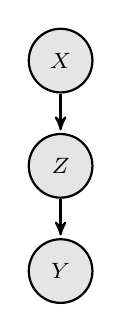
\begin{tikzpicture}[->,>=stealth',shorten >=1pt,auto,node distance=.5cm,
  thick,main node/.style={observed}]
\node[main node](1){$X$};
\node[main node, below =of 1](2){$Z$};
\node[main node, below =of 2](3){$Y$};
 \path[every node/.style={font=\sffamily\small}]
    (1) edge node {} (2)
    (2) edge node {} (3);	
\end{tikzpicture}
\end{subfigure}
\begin{subfigure}[t]{0.2\textwidth}
\centering
\caption{$X \ci Y|Z$}
\label{fig:dseptripple2}
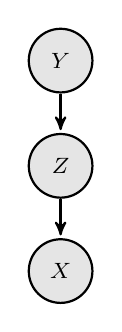
\begin{tikzpicture}[->,>=stealth',shorten >=1pt,auto,node distance=.5cm,
  thick,main node/.style={observed}]
\node[main node](1){$Y$};
\node[main node, below =of 1](2){$Z$};
\node[main node, below =of 2](3){$X$};
 \path[every node/.style={font=\sffamily\small}]
    (1) edge node {} (2)
    (2) edge node {} (3);	
\end{tikzpicture}
\end{subfigure}
\begin{subfigure}[t]{0.2\textwidth}
\centering
\caption{$X \ci Y|Z$}
\label{fig:dseptripple3}
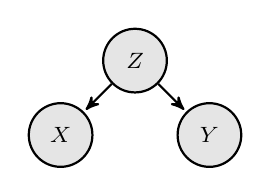
\begin{tikzpicture}[->,>=stealth',shorten >=1pt,auto,node distance=.5cm,
  thick,main node/.style={observed}]
\node[main node](1){$Z$};
\node[main node, below left =of 1](2){$X$};
\node[main node, below right=of 1](3){$Y$};
 \path[every node/.style={font=\sffamily\small}]
    (1) edge node {} (2)
        edge node {} (3);	
\end{tikzpicture}
\end{subfigure}
\begin{subfigure}[t]{0.2\textwidth}
\centering
\caption{$X \ci Y|\{\}$}
\label{fig:dseptripple4}
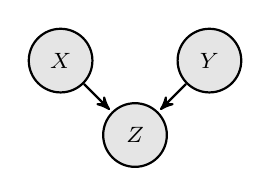
\begin{tikzpicture}[->,>=stealth',shorten >=1pt,auto,node distance=.5cm,
  thick,main node/.style={observed}]
\node[main node](1){$Z$};
\node[main node, above left =of 1](2){$X$};
\node[main node, above right =of 1](3){$Y$};
 \path[every node/.style={font=\sffamily\small}]
    (2) edge node {} (1)
    (3) edge node {} (1);	
\end{tikzpicture}
\end{subfigure}
\end{figure}

\vspace{.3cm}
\begin{definition}[unblocked path]
\label{def:unblocked}
A path from $X$ to $Y$ is a sequence of edges linking adjacent nodes starting at $X$ and finishing at $Y$,  $(X,V_{1},V_{2}...V_{k},Y)$. It is unblocked if every triple, $X-V_{1}-V_{2},V_{1}-V_{2}-V{3},...,V_{k-1}-V_{k}-Y$ in the path is unblocked (each triple will belong to one of the cases in figure \ref{fig:dseptriples})
\end{definition}

\vspace{.3cm}
\begin{definition}[d-separation]
\label{def:dsep}
The variables $\boldsymbol{X}$ are d-separated from $\boldsymbol{Y}$ given $\boldsymbol{Z}$ in the network $G$ if, there are no unblocked paths from any $X \in \boldsymbol{X}$ to any $Y \in \boldsymbol{Y}$ after conditioning on $\boldsymbol{Z}$. 
\end{definition}

\vspace{.3cm}
\begin{theorem}[d-separation and conditional independence]
\label{thrm:dsep_independence}
If a set of variables $\boldsymbol{Z}$ d-separates $\boldsymbol{X}$ and $\boldsymbol{Y}$ in a Bayesian network $G$ then ${(\boldsymbol{X} \ci \boldsymbol{Y}|\boldsymbol{Z})}$ in all distributions $P$ compatible with $G$. Conversely, if $\boldsymbol{X}$ and $\boldsymbol{Y}$ are d-connected (not d-separated) given $\boldsymbol{Z}$ then it is possible to construct a distribution $P'$ that factorises over $G$ in which they are dependent. 
\end{theorem}

Theorem \ref{thrm:dsep_independence} says that independencies implied by d-separation on a graph hold in every distribution that can be factored over that graph and that if ${(\boldsymbol{X} \ci \boldsymbol{Y}|\boldsymbol{Z})}$ in \emph{all} distributions that can be factored over $G$ then they are d-separated in $G$. If we denote the independencies implied by d-separation in a graph by $\indep{G}$ and the set of independencies in a distribution by $\indep{P}$ then $\indep{G} \subseteq \indep{P}$. 

If $\indep{G} = \indep{P}$ then $G$ is called a perfect map for $P$. However, it is possible to construct distributions that do not have a perfect map, that is they contain conditional independencies that cannot be represented by d-separation. A particular case in which this occurs is when there are deterministic relationships between variables. If we have a Bayesian network $G$ in which we specify that some nodes are deterministic we cannot conclude that if $X$ and $Y$ are d-connected then there exists a distribution $P'$ \emph{consistent} with $G$ in which they are dependent. This does not conflict with theorem \ref{thrm:dsep_independence} as \emph{consistent} in this setting requires that $P'$ both factorises over $G$ and satisfies the specified the deterministic relations between variables. This subtlety led to confusion in assessing what independencies hold between counterfactuals via twin networks \citep{Pearl2000,Richardson2013} and demonstrates the caution required in using d-connecteness to assert lack of independence. D-separation can be extended to compute the additional independencies implied by a graph in which certain nodes are known to be deterministic \citep{Geiger1990}. 

\section{The Do Calculus} 
\label{sec:do_calculus}

The do-calculus is a set of three rules \citep{Pearl1995} that can be applied to simplify the expression for an interventional distribution. If by repeated application of the do-calculus, along with standard probability transformations, we can obtain an expression containing only observational quantities then we can use it to estimate the interventional distribution from observational data. Let $\boldsymbol{X}$,$\boldsymbol{Y}$,$\boldsymbol{Z}$ and $\boldsymbol{W}$ be disjoint sets of variables in a causal graph $G$. We denote the graph $G$ after the an intervention $do(\boldsymbol{X})$, which has the effect of removing all edges into variables in $\boldsymbol{X}$, as $G_{\overline{\boldsymbol{X}}}$

\subsubsection{Rule 1: (adding or removing evidence)} 

Rule 1 allows us to remove (or insert) observational evidence from the right hand side of a conditional interventional distribution. It follows directly from the fact that the relationship between d-separation in a network and independence in the corresponding probability distribution still applies after an intervention. 


If $(\boldsymbol{Y} \ci \boldsymbol{W} | \boldsymbol{Z},\boldsymbol{X})$ in $G_{\overline{\boldsymbol{X}}}$:
\eqn{
\label{eq:Do1}
 P(\boldsymbol{Y}|do(\boldsymbol{X}=\boldsymbol{x}),\boldsymbol{Z}=\boldsymbol{z},\boldsymbol{W}=\boldsymbol{w}) = P(\boldsymbol{Y}|do(\boldsymbol{X}=\boldsymbol{x}),\boldsymbol{Z}=\boldsymbol{z}) 
}


\begin{figure}[h]
\centering
\caption{Rule 1 example. $(Y \ci W|X)$ in  $G_{\overline{\boldsymbol{X}}} \implies \P{Y|do(X),W} = \P{Y|do(X)}$ }
\label{fig:mutilatednet}
\begin{subfigure}[t]{0.3\textwidth}
\centering
\caption{original network, $G$}
\label{fig:mutilatedOriginal}
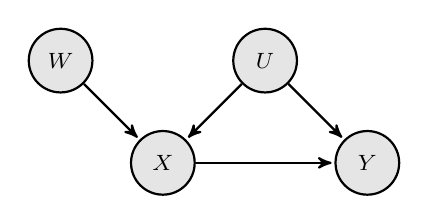
\begin{tikzpicture}[->,>=stealth',shorten >=1pt,auto,node distance=1cm,
  thick,main node/.style={observed}]

 %nodes
\node[main node](1){$U$};
\node[main node, below left=of 1](2){$X$};
\node[main node, below right=of 1](3){$Y$};
\node[main node, above left=of 2](4){$W$};


 \path[every node/.style={font=\sffamily\small}]
    (1) edge node {} (2)
    	edge node {} (3)
    (2) edge node {} (3)
    (4) edge node {} (2);
	
\end{tikzpicture} 
\end{subfigure}
\begin{subfigure}[t]{0.5\textwidth}
\centering
\caption{network after the intervention $do(X=x)$, $G_{\overline{X}}$}
\label{fig:mutilatedAfter}
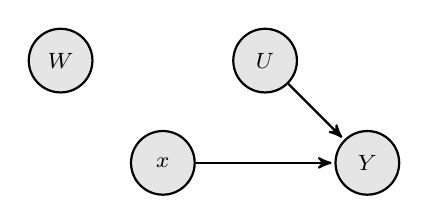
\begin{tikzpicture}[->,>=stealth',shorten >=1pt,auto,node distance=1cm,
  thick,main node/.style={observed}]

 %nodes
\node[main node](1){$U$};
\node[main node, below left=of 1](2){$x$};
\node[main node, below right=of 1](3){$Y$};
\node[main node, above left=of 2](4){$W$};


 \path[every node/.style={font=\sffamily\small}]
    (1) edge node {} (3)
    (2) edge node {} (3);
    
\end{tikzpicture}
\end{subfigure}
\end{figure}

\subsubsection{Rule 2: (exchanging actions with observations)}
Rule 2 describes when conditioning on $\boldsymbol{X} = \boldsymbol{x}$ and intervening, $do(\boldsymbol{X}=\boldsymbol{x})$, have the same effect on the distribution over $\boldsymbol{Y}$. Let $G_{\underline{\boldsymbol{X}}}$ denote the causal graph $G$ with all edges \emph{leaving} $X$ removed.

If  $(\boldsymbol{Y} \ci \boldsymbol{X}|\boldsymbol{W})$ in $G_{\underline{\boldsymbol{X}}}$:
\eqn{
\label{eq:Do22}
P(\boldsymbol{Y}|do(\boldsymbol{X}=\boldsymbol{x}),\boldsymbol{W}) = P(\boldsymbol{Y}|\boldsymbol{X}=\boldsymbol{x},\boldsymbol{W})
}

The intuition behind this is that interventional distributions differ from observational ones due to the presence of indirect paths between $X$ and $Y$. Observing a variable $X$ provides information about $Y$ both directly and indirectly, by changing our belief about the distribution of the parents of $X$. However setting $X$ tells us nothing about its parents and therefor affects $Y$ only via direct paths out of $X$. Removing edges \emph{leaving} $X$ removes all the direct paths out of $X$. If $X$ is then independent of $Y$ (conditional on $W$), that indicates there are no indirect paths. This implies conditioning on $X$ is equivalent to setting $X$ (given $W$).

Equation \ref{eq:Do22} does not cover cases where acting on one set of variables allows us to replace acting on another set with conditioning (see figure \ref{fig:rule2_2}). The general form of rule 2 is given in equation \ref{eq:Do2}.

If  $(\boldsymbol{Y} \ci \boldsymbol{X}|\boldsymbol{W},\boldsymbol{Z})$ in $G_{\underline{\boldsymbol{X}}\overline{\boldsymbol{Z}}}$:
\eqn{
\label{eq:Do2}
P(\boldsymbol{Y}|do(\boldsymbol{X}=\boldsymbol{x}),
do(\boldsymbol{Z}=\boldsymbol{z}),
\boldsymbol{W}) = P(\boldsymbol{Y}|\boldsymbol{X}=\boldsymbol{x},do(\boldsymbol{Z}=\boldsymbol{z}),\boldsymbol{W})
}

\begin{figure}[h]
\centering
\caption{An example of rule 2 with a single intervention $(Y \ci X|W)$ in  $G_{\underline{\boldsymbol{X}}} \implies \P{Y|do(X),W} = \P{Y|X,W}$. In this example, observing $X$ provides information about $Y$ both directly and indirectly, because knowing $X$ tells us something about $W$ which also influences $Y$. If we condition on $W$, we block this indirect path.}
\label{fig:rule2}
\begin{subfigure}[t]{0.29\textwidth}
\centering
\caption{original network, $G$}
\label{fig:rule2_orig}
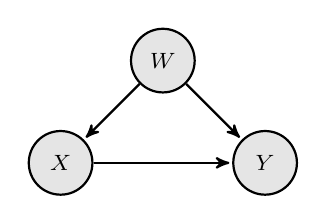
\begin{tikzpicture}[->,>=stealth',shorten >=1pt,auto,node distance=1cm,
  thick,main node/.style={observed}]

 %nodes
\node[main node](1){$W$};
\node[main node, below left=of 1](2){$X$};
\node[main node, below right=of 1](3){$Y$};
 \path[every node/.style={font=\sffamily\small}]
    (1) edge  (2)  edge  (3)
    (2) edge (3);
\end{tikzpicture} 
\end{subfigure}
\begin{subfigure}[t]{0.29\textwidth}
\centering
\caption{$G_{\overline{X}}$}
\label{fig:rule2_after}
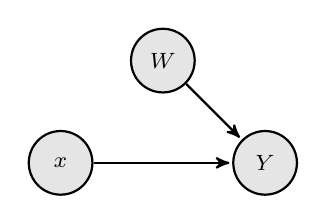
\begin{tikzpicture}[->,>=stealth',shorten >=1pt,auto,node distance=1cm,
  thick,main node/.style={observed}]

 %nodes
\node[main node](1){$W$};
\node[main node, below left=of 1](2){$x$};
\node[main node, below right=of 1](3){$Y$};


 \path[every node/.style={font=\sffamily\small}]
    (1)	edge (3)
    (2) edge (3);
\end{tikzpicture} 
\end{subfigure}
\begin{subfigure}[t]{0.29\textwidth}
\centering
\caption{$G_{\underline{X}}$}
\label{fig:rule2_indirect}
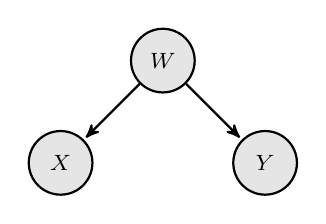
\begin{tikzpicture}[->,>=stealth',shorten >=1pt,auto,node distance=1cm,
  thick,main node/.style={observed}]

 %nodes
\node[main node](1){$W$};
\node[main node, below left=of 1](2){$X$};
\node[main node, below right=of 1](3){$Y$};


 \path[every node/.style={font=\sffamily\small}]
    (1) edge  (2)
    	edge  (3);
    
\end{tikzpicture} 
\end{subfigure}
\end{figure}

\begin{figure}[h]
\centering
\caption{An example of applying equation \ref{eq:Do2}. In this case $(Y \ci X|Z) \text{ in } G_{\underline{X}\overline{Z}}\implies \P{Y|do(X=x),do(Z=z)} = \P{Y|X=x,do(Z=z)}$. Observing, rather than intervening, on $Z$ would not have allowed us to exchange $do(X=x)$ for $X=x$. Conditioning on $Z$ does block the indirect path $X-Z-V-Y$ but opens $X-U-Z-V-Y$.  }
\label{fig:rule2_2}
\begin{subfigure}[t]{0.29\textwidth}
\centering
\caption{original network, $G$}
\label{fig:rule22_orig}
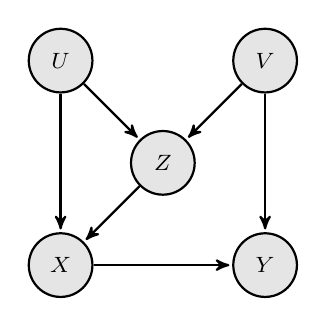
\begin{tikzpicture}[->,>=stealth',shorten >=1pt,auto,node distance=1cm,
  thick,main node/.style={observed}]

 %nodes
\node[main node](1){$Z$};
\node[main node, below left=of 1](2){$X$};
\node[main node, below right=of 1](3){$Y$};
\node[main node, above left=of 1](4){$U$};
\node[main node, above right=of 1](5){$V$};
 \path[every node/.style={font=\sffamily\small}]
    (1) edge  (2)
    (2) edge (3)
    (4) edge (1) edge (2)
    (5) edge (1) edge (3);
\end{tikzpicture} 
\end{subfigure}
\begin{subfigure}[t]{0.29\textwidth}
\centering
\caption{after $do(Z)$, $G_{\overline{Z}}$}
\label{fig:rule22_after}
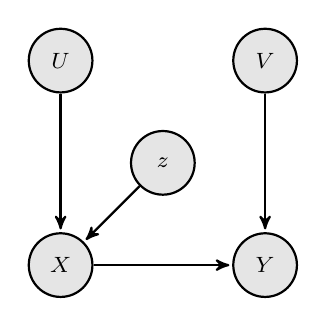
\begin{tikzpicture}[->,>=stealth',shorten >=1pt,auto,node distance=1cm,
  thick,main node/.style={observed}]

 %nodes
\node[main node](1){$z$};
\node[main node, below left=of 1](2){$X$};
\node[main node, below right=of 1](3){$Y$};
\node[main node, above left=of 1](4){$U$};
\node[main node, above right=of 1](5){$V$};
 \path[every node/.style={font=\sffamily\small}]
    (1) edge  (2)
    (2) edge (3)
    (4) edge (2)
    (5) edge (3);
\end{tikzpicture} 
\end{subfigure}
\begin{subfigure}[t]{0.29\textwidth}
\centering
\caption{$G_{\underline{X}\overline{Z}}$}
\label{fig:rule22_indirect}
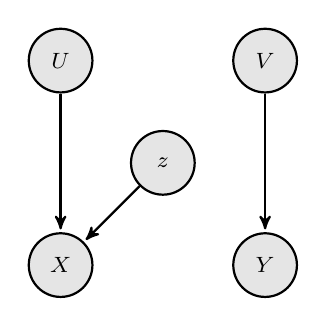
\begin{tikzpicture}[->,>=stealth',shorten >=1pt,auto,node distance=1cm,
  thick,main node/.style={observed}]

 %nodes
\node[main node](1){$z$};
\node[main node, below left=of 1](2){$X$};
\node[main node, below right=of 1](3){$Y$};
\node[main node, above left=of 1](4){$U$};
\node[main node, above right=of 1](5){$V$};
 \path[every node/.style={font=\sffamily\small}]
    (1) edge  (2)
    (4) edge (2)
    (5) edge (3);
\end{tikzpicture} 
\end{subfigure}
\end{figure}

\subsubsection{Rule 3: (adding or removing actions)}
This rule describes cases where the intervention $do(\boldsymbol{X}=\boldsymbol{x})$ has no effect on the distribution of the outcome $\boldsymbol{Y}$. A simple case of rule 3 is given in equation \ref{eq:Do3_1}. If $\boldsymbol{Y}$ is independent of $\boldsymbol{{X}}$ in $G$ after removing links entering $\boldsymbol{X}$ then can be no direct path from $\boldsymbol{X}$ to $\boldsymbol{Y}$ and any intervention on $\boldsymbol{X}$ will not affect $\boldsymbol{Y}$.

if $(\boldsymbol{Y} \ci \boldsymbol{{X}})$ in $G_{\boldsymbol{\overline{X}}}$:

\eqn{
\label{eq:Do3_1}
\P{\boldsymbol{Y}|do(\boldsymbol{X}=\boldsymbol{x})} = \P{\boldsymbol{Y}}
}

The general case of rule 3 is easier to state by explicitly representing the intervention in the graphical model. Let $G^{\boldsymbol{\hat{X}}}$ denote the graph $G$ after adding a variable $\hat{X_i}$ as a parent of each variable $X_i \in \boldsymbol{X}$ (see figure \ref{fig:rule3_augmented}). The variable $\hat{X_i}$ can be thought of as representing the mechanism by which $X_i$ takes its value, either by being set via intervention or as a stochastic function of its other parents \citep{Koller2009}.


if $(\boldsymbol{Y} \ci \boldsymbol{\hat{X}} |\boldsymbol{Z},\boldsymbol{W})$ in $G^{\boldsymbol{\hat{X}}}_{\boldsymbol{\overline{Z}}}$:
\eqn{
\label{eq:Do3}
P(\boldsymbol{Y}|do(\boldsymbol{Z}=\boldsymbol{z}),do(\boldsymbol{X}=\boldsymbol{x}),\boldsymbol{W}=\boldsymbol{w}) = P(\boldsymbol{Y}|do(\boldsymbol{Z}=\boldsymbol{z}),\boldsymbol{W}=\boldsymbol{w})
}

The statement that $\boldsymbol{Y} \ci \boldsymbol{\hat{X}}$ (without conditioning on $\boldsymbol{X}$) implies that there is no unblocked path from $\boldsymbol{X}$ to $\boldsymbol{Y}$ in $G$ which \emph{includes} an arrow leaving $\boldsymbol{X}$. These are the only paths by which intervening in $\boldsymbol{X}$ can effect $\boldsymbol{Y}$.

\begin{figure}[h]
\centering
\caption{Example application of equation \ref{eq:Do3}. $(Y \ci \hat{X}|W,Z) \implies \P{Y|do(X),W,Z} = \P{Y|W,Z}$. We have to condition on $Z$ because conditioning on $W$ blocks the path $\hat{X}-X-W-Y$ but opens $\hat{X}-X-Z-Y$.}
\label{fig:rule3}
\begin{subfigure}[t]{0.29\textwidth}
\centering
\caption{original network, $G$}
\label{fig:rule3_original}
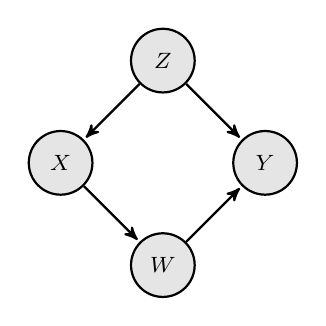
\begin{tikzpicture}[->,>=stealth',shorten >=1pt,auto,node distance=1cm,
  thick,main node/.style={observed}]
 %nodes
\node[main node](1){$Z$};
\node[main node, below left=of 1](2){$X$};
\node[main node, below right=of 1](3){$Y$};
\node[main node, below right=of 2](4){$W$};
 \path[every node/.style={font=\sffamily\small}]
    (1) edge (2) edge (3)
    (2) edge (4)
    (4) edge (3);
\end{tikzpicture} 
\end{subfigure}
\begin{subfigure}[t]{0.29\textwidth}
\centering
\caption{augmented graph $G^{\hat{X}}$}
\label{fig:rule3_augmented}
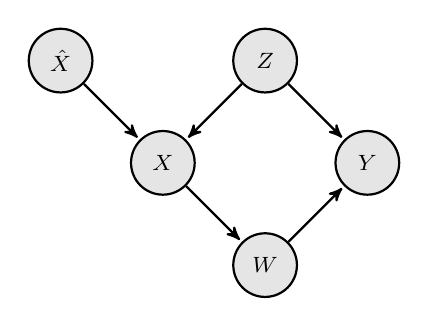
\begin{tikzpicture}[->,>=stealth',shorten >=1pt,auto,node distance=1cm,
  thick,main node/.style={observed}]
 %nodes
\node[main node](1){$Z$};
\node[main node, below left=of 1](2){$X$};
\node[main node, below right=of 1](3){$Y$};
\node[main node, below right=of 2](4){$W$};
\node[main node, above left=of 2](5){$\hat{X}$};
 \path[every node/.style={font=\sffamily\small}]
    (1) edge (2) edge (3)
    (2) edge (4)
    (4) edge (3)
    (5) edge (2);
\end{tikzpicture} 
\end{subfigure}
\begin{subfigure}[t]{0.29\textwidth}
\centering
\caption{$G_{\overline{X}}$}
\label{fig:rule3_after}
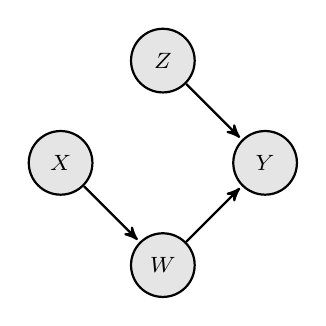
\begin{tikzpicture}[->,>=stealth',shorten >=1pt,auto,node distance=1cm,
  thick,main node/.style={observed}]
 %nodes
\node[main node](1){$Z$};
\node[main node, below left=of 1](2){$X$};
\node[main node, below right=of 1](3){$Y$};
\node[main node, below right=of 2](4){$W$};
 \path[every node/.style={font=\sffamily\small}]
    (1) edge (3)
    (2) edge (4)
    (4) edge (3);
\end{tikzpicture} 
\end{subfigure}
\end{figure}


\subsection{Identifiability}
A natural question to ask is, given a set of assumptions about the causal graph, is it possible to estimate a given interventional distribution from observational data? This is the identifiablity problem. It asks if we can obtain an unbiased point estimate for the causal query of interest in the infinite data limit. A query is non-parametrically identifiable if it is identifiable without  assumptions about the functional form of the dependencies between variables in the graph.

\vspace*{.3cm}
\begin{definition}[Non-parametric identifiablity]
Let $G$ be a causal graph containing observed variables $\boldsymbol{V}$ and latent variables $\boldsymbol{U}$ and let $\P{\cdot}$ be any positive distribution over $\boldsymbol{V}$. A causal query of the form $\P{\boldsymbol{Y}|do(\boldsymbol{X}),\boldsymbol{W}}$, where $\boldsymbol{Y}$,$\boldsymbol{X}$ and $\boldsymbol{W}$ are disjoint subsets of $\boldsymbol{V}$, is non-parametrically identifiable if it is uniquely determined by $\P{\cdot}$ and $G$.
\end{definition} 

The question of non-parametric identifiability is solved. The do calculus is complete \cite{Shpitser2006b,Huang2006}. A problem is identifiable if and only if the interventional distribution of interest can be transformed into term containing only observational quantities via repeated application of the do-calculus. There is a polynomial time algorithm \cite{Shpitser2006a} based on these properties that, for a given network and interventional (do-type) query, can:

\begin{enumerate}
\item determine if the query can be translated into an expression involving only distributions over observed variables. In other words, determine if the query is identifiable given the assumptions encoded by the network, and
\item if it is identifiable, return the required expression. 
\end{enumerate}

Figure \ref{fig:identify} shows some examples of identifiable and non identifiable queries. I have created a javascript implementation of the identifiability algorithm \cite{Shpitser2006a} on which you can test your own queries http://finnhacks42.github.io.

\begin{figure}[h]
\centering
\caption{Examples of identifiable and non-identifiable queries. In subfigures (a), (b) and (c) the causal query $\P{Y|do(X)}$ is identifiable. In subfigures (d), (e) and (f) it is not.}
\label{fig:identify}
\begin{subfigure}[t]{0.29\textwidth}
\centering
\caption{}
\label{fig:id1}
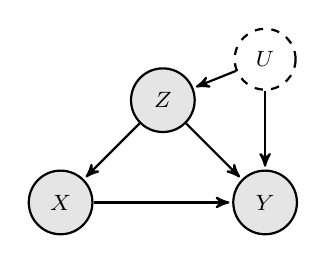
\begin{tikzpicture}[->,>=stealth',shorten >=1pt,auto,node distance=1cm,
  thick,lt/.style={latent},ob/.style={observed}]
\node[ob](1){$Z$};
\node[ob, below left=of 1](2){$X$};
\node[ob, below right=of 1](3){$Y$};
\node[lt,above=of 3](4){$U$};
 \path[every node/.style={font=\sffamily\small}]
    (1) edge (2) edge (3)
    (2) edge (3)
    (4) edge (1) edge (3);
\end{tikzpicture} 
\end{subfigure}
\begin{subfigure}[t]{0.29\textwidth}
\centering
\caption{}
\label{fig:id2}
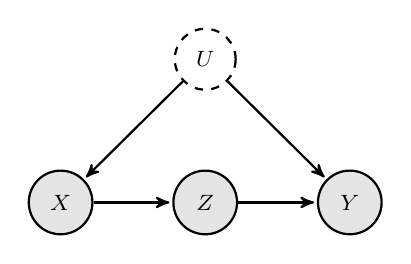
\begin{tikzpicture}[->,>=stealth',shorten >=1pt,auto,node distance=1cm,
  thick,lt/.style={latent},ob/.style={observed}]
\node[ob](1){$X$};
\node[ob, right=of 1](2){$Z$};
\node[ob, right=of 2](3){$Y$};
\node[lt,above=of 2](4){$U$};
 \path[every node/.style={font=\sffamily\small}]
    (1) edge (2)
    (2) edge (3)
    (4) edge (1) edge (3);
\end{tikzpicture} 
\end{subfigure}
\begin{subfigure}[t]{0.29\textwidth}
\centering
\caption{}
\label{fig:id3}
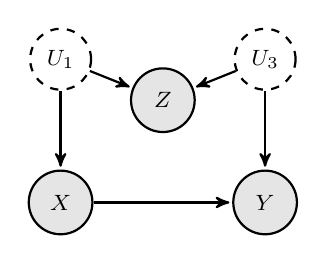
\begin{tikzpicture}[->,>=stealth',shorten >=1pt,auto,node distance=1cm,
  thick,lt/.style={latent},ob/.style={observed}]
\node[ob](1){$Z$};
\node[ob, below left=of 1](2){$X$};
\node[ob, below right=of 1](3){$Y$};
\node[lt,above=of 3](4){$U_3$};
\node[lt,above=of 2](5){$U_1$};
 \path[every node/.style={font=\sffamily\small}]
    (2) edge (3)
    (4) edge (1) edge (3)
    (5) edge (2) edge (1);
\end{tikzpicture} 
\end{subfigure}
\begin{subfigure}[t]{0.29\textwidth}
\centering
\vspace*{.5cm}
\caption{}
\label{fig:nid1}
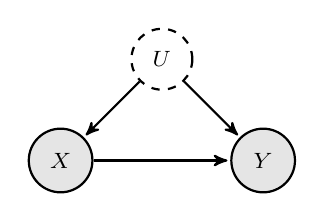
\begin{tikzpicture}[->,>=stealth',shorten >=1pt,auto,node distance=1cm,
  thick,lt/.style={latent},ob/.style={observed}]
\node[lt](1){$U$};
\node[ob, below left=of 1](2){$X$};
\node[ob, below right=of 1](3){$Y$};
 \path[every node/.style={font=\sffamily\small}]
    (1) edge (2) edge (3)
    (2) edge (3);
\end{tikzpicture} 
\end{subfigure}
\begin{subfigure}[t]{0.29\textwidth}
\centering
\vspace*{.5cm}
\caption{}
\label{fig:nid2_instrumental_variable}
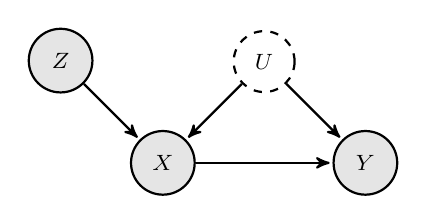
\begin{tikzpicture}[->,>=stealth',shorten >=1pt,auto,node distance=1cm,
  thick,lt/.style={latent},ob/.style={observed}]
\node[lt](1){$U$};
\node[ob, below left=of 1](2){$X$};
\node[ob, below right=of 1](3){$Y$};
\node[ob, above left=of 2](4){$Z$};
 \path[every node/.style={font=\sffamily\small}]
    (1) edge (2) edge (3)
    (2) edge (3)
    (4) edge (2);
\end{tikzpicture} 
\end{subfigure}
\begin{subfigure}[t]{0.29\textwidth}
\centering
\vspace*{.5cm}
\caption{}
\label{fig:nid3}
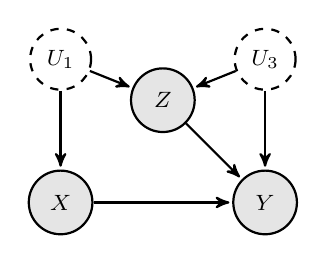
\begin{tikzpicture}[->,>=stealth',shorten >=1pt,auto,node distance=1cm,
  thick,lt/.style={latent},ob/.style={observed}]
\node[ob](1){$Z$};
\node[ob, below left=of 1](2){$X$};
\node[ob, below right=of 1](3){$Y$};
\node[lt,above=of 3](4){$U_3$};
\node[lt,above=of 2](5){$U_1$};
 \path[every node/.style={font=\sffamily\small}]
    (2) edge (3)
    (4) edge (1) edge (3)
    (5) edge (2) edge (1)
    (1) edge (3);
\end{tikzpicture} 
\end{subfigure}
\end{figure}


Many interesting questions relating to identifiability remain open. What is the minimal (by some metric) additional information that would be required to make a non-identifiable query identifiable? What if we assume various restrictions on the functional form of the relationships between the variables? Some queries which are not identifiable non-parametrically can be identified by additional assumptions such as linearity. A complete algorithm for the problem of linear identifiability is yet to be found, despite a rich body of work \citep{Chen2016,tian2009parameter,drton2011global}.

Although identifiability is a natural and important question to ask, it does not partition causal questions into solvable and unsolvable. Estimators for identifiable queries can be slow to converge and we may be able to obtain useful bounds on causal effects in cases where point estimates are not identified.


\section{Estimation}
\subsection{Defining causal effects} 
So far we have described causal effect estimation in term of identifying the interventional distribution $\P{Y|do(X)}$ from observational data. This interventional distribution is in fact a family of distributions parameterised by the value, $x$, to which the treatment variable $X$ is set. From a decision theoretic viewpoint, we can select an optimal action $x$ by specifying a utility function $\mathcal{U}:y \in \mathcal{Y} \rightarrow \mathbb{R}$ that assigns a value to each outcome $y$ and then selecting the action that maximises the expected utility. 

\eqn{
\label{eqn:utility_max}
x* =\argmax_x \Esub{y\sim\P{Y|do(X=x)}}{{\cal{U}}(y)}
} 

Frequently however, studies wish to define and estimate a causal effect without reference to a specific utility function. There are a variety of ways of defining causal effects that can be viewed as different ways of summarising the family of interventional distributions. For a binary treatment variable $X$, the average causal effect, ACE \footnote{also referred to as the average treatment effect (ATE)} is defined as:

\eqn{
\label{eqn:ACE}
ACE = \E{Y|do(X = 1)} - \E{Y|do(X=0)}
}

Assuming the expectations in equation \ref{eqn:ACE} are well defined, the ACE captures the shift in the mean outcome that arises from varying $X$. It does not capture changes in variance or higher moments of the distribution. The ACE can be generalised to non-discrete interventions by considering the effect on the expectation of $Y$ of an infinitesimal change in $x$. If $X$ is linearly related to $Y$ then the ACE is constant and equivalent to the corresponding coefficient in the linear structural equation model. 

\eqn{
\label{eqn:ACE_continuous}
ACE(x) = \frac{d}{dx}\E{Y|do(X=x)}
}


The average causal effect is often introduced as the average over individual causal effects as discussed in section \ref{sec:counterfactuals}. Individual causal effects are deterministic and cannot be expressed as properties of the interventional distribution. However we can personalise the average causal effect by stating it with respect to some observed context. I will refer to this as the personalised causal effect (PCE).\footnote{This quantity is sometimes called the conditional average treatment effect (CATE), however that term is also used for the sample rather than population effect.} 

\eqn{
PCE(z) = \E{Y|do(X=1),z} - \E{Y|do(X=0),z}
}

In some cases we may be interested in the average causal effect for some sub-group of the population. A particularly common example of this is the average treatment effect of the treatment of the treated (ATT). This would be the key quantity of interest if we had to decide whether or not to continue providing a program or treatment for which we could not control the treatment assignment process. 

\eqn{
ATT = \Esub{z\sim \P{Z|x=1}}{Y|do(X = 1)} - \Esub{z\sim \P{Z|x=1}}{Y|do(X=0)}
}

Causal effects can also be written in terms of counterfactuals. The ACE is $\E{\cf{Y}{1} - \cf{Y}{0}}$. We could estimate the ratio of expectations $\frac{\E{\cf{Y}{1}}}{\E{\cf{Y}{0}}}$ instead of the difference. However, the quantity   $\E{\frac{\cf{Y}{1}}{\cf{Y}{0}}}$ depends on the joint distribution over the counterfactual variables $(\cf{Y}{1},\cf{Y}{0})$ and thus cannot be computed from the interventional distribution. 

Another way of conceptualising causal effects is as a property indicating the strength of the causal link between two variables. This notion is complex to formalise when the relationship between variables is non-linear. Suppose $Y = X \oplus Z$ with $P(Z=1)=\frac{1}{2}$, the interventional distributions over $X$ are identical after marginalising out $Z$. \citet{Janzing2013} propose a number of postulates that a notion of causal strength could satisfy, demonstrate why previous measures fail these postulates and propose an alternative based on information flow. 


\subsection{Estimating causal effects by adjusting for confounding variables}
\label{sec:causal_effect_under_ignorability}
Probably the two most frequently applied approaches to estimating causal effects from observational data are instrumental variables and adjusting for confounding factors. Instrumental variables correspond to the graph in figure \ref{fig:nid2_instrumental_variable}, which is not identifiable without parametric assumptions, however they can provide tight bounds. Adjusting for confounding equates to identifying a set of variables $\boldsymbol{Z}$ such that the ignorability assumption discussed in section \ref{sec:counterfactuals} holds. This corresponds to a simple graphical test known as the backdoor criterion \citep{Pearl2000}. The setting is also referred to as unconfounded. 

\vspace*{0.3cm}
\begin{theorem}[The backdoor criterion]\citep{Pearl2000}
Let $\boldsymbol{X}$, $\boldsymbol{Z}$ and $\boldsymbol{Y}$ be disjoint sets of vertices in a causal graph $G$. If $\boldsymbol{Z}$ blocks (see Definition \ref{def:unblocked}) for every path from $X_i$ to $Y_j$ that contains a link into $X_i$, for every pair $(X_i \in \boldsymbol{X},Y_j \in \boldsymbol{Y})$, and no node in $\boldsymbol{Z}$ is a decedent of a node in $\boldsymbol{X}$ then the backdoor criterion is satisfied and;

\eqn{
\label{eqn:backdoor}
\P{\boldsymbol{y}|do(\boldsymbol{x})} =\sum_{\boldsymbol{z}} \P{\boldsymbol{y}|\boldsymbol{x},\boldsymbol{z}}\P{\boldsymbol{z}}
}
\end{theorem}

The backdoor criterion derives from rule 2 of the do-calculus. Selecting which covariates should be adjusted for to estimate a causal effect reduces to identifying a set which satisfies the backdoor criterion. There may be more than one valid adjustment set, see figure \ref{fig:adjust_multiple}. The seemingly simple problem of determining if a variable should be adjusted for when estimating causal effects has been the subject of substantial debate and controversy \citep{pearl2009myth}. Adjusting for the wrong variables (even pre-treatment variables) can introduce or magnify bias, see figure \ref{fig:m-graph}. Causal graphs and the back door criterion provide a clear mechanism for deciding which variables should be adjusted for. For a practical example, see the discussion in \citet{schisterman2009overadjustment} on whether birth weight should be adjusted for to estimate the causal effect of smoking on neonatal mortality.  

\begin{figure}
\centering
\caption{}
\label{fig:adjustment}
\begin{subfigure}[t]{0.48\textwidth}
\centering
\caption{There can be multiple valid adjustment sets. $Z_1$ or $Z_2$ or $\set{Z_1,Z_2}$ all block the backdoor path from $X$ to $Y$.}
\label{fig:adjust_multiple}
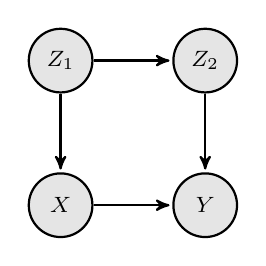
\begin{tikzpicture}[->,>=stealth',shorten >=1pt,auto,node distance=1cm,
  thick,lt/.style={latent},ob/.style={observed}]
\node[ob](2){$X$};
\node[ob, right=of 2](3){$Y$};
\node[ob,above=of 3](4){$Z_2$};
\node[ob,above=of 2](5){$Z_1$};
 \path[every node/.style={font=\sffamily\small}]
    (2) edge (3)
    (5) edge (2) edge (4)
    (4) edge (3);
\end{tikzpicture} 
\end{subfigure}
\begin{subfigure}[t]{0.48\textwidth}
\centering
\caption{Conditioning on $Z$ opens the backdoor path $X-U_1-Z-U_2-Y$}
\label{fig:m-graph}
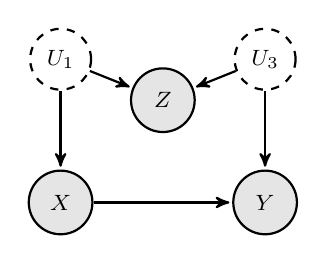
\begin{tikzpicture}[->,>=stealth',shorten >=1pt,auto,node distance=1cm,
  thick,lt/.style={latent},ob/.style={observed}]
\node[ob](1){$Z$};
\node[ob, below left=of 1](2){$X$};
\node[ob, below right=of 1](3){$Y$};
\node[lt,above=of 3](4){$U_3$};
\node[lt,above=of 2](5){$U_1$};
 \path[every node/.style={font=\sffamily\small}]
    (2) edge (3)
    (4) edge (1) edge (3)
    (5) edge (2) edge (1);
\end{tikzpicture} 
\end{subfigure}
\end{figure}

Given that a set of variables $\boldsymbol{Z}$ satisfies the backdoor criterion (or equivalently the conditional ignorability assumption), the interventional distribution is asymptotically identifiable and can be estimated from equation \ref{eqn:backdoor}. The expected value of $Y$ after the intervention $do(X=x)$ is given by equation \ref{eqn:expected_post_intervention} and the average causal effect for a binary intervention $x \in \set{0,1}$ is given by equation \ref{eqn:ace_ignoreable}.

\eqn{
\label{eqn:expected_post_intervention}
\E{Y|do(X=x)} = \Esub{z\sim \P{\vb{Z}}}{\E{Y|x,\vb{z}}}
} 

\eqn{
\label{eqn:ace_ignoreable}
ACE = \Esub{z\sim \P{\vb{Z}}}{\E{Y|1,\vb{z}}-\E{Y|0,\vb{z}}}
}  

Assuming $x$ and $\vb{z}$ are discrete, equation \ref{eqn:expected_post_intervention}, and thus the ACE, can be estimated by selecting the data for which $X=x$, stratifying by $\vb{Z}$, then computing the mean outcome within each stratum and finally weighting the results by the number of samples in each strata. However this approach is not workable for most real world problems with finite samples as the number of strata grows exponentially with the dimension of $\vb{Z}$ and it cannot handle continuous covariates. There is a substantial body of work within in the statistics and econometrics literature on estimating average causal effects assuming conditional ignorability, see \citet{Imbens2004} for a comprehensive review. The key approaches are based on matching on covariates, propensity score methods and regression. We now examine these approaches from a machine learning perceptive. 

In standard supervised learning, we have a training set $(\vb{x_1},y_1),...,(\vb{x_n},y_n)$ assumed to be sampled i.i.d from an unknown distribution $\P{\vb{x},y} =\P{\vb{x}}\P{y|\vb{x}}$. The goal is to select a hypothesis $h \in \mathcal{H} : \mathcal{X} \rightarrow \mathcal{Y}$ such that, on unseen data $ \sim \P{\vb{x},y}$, $h(\vb{x})$ is close (by some metric) in expectation to $y$. In other words we wish to minimise the generalisation error $E_{out}(h)$,

\eqn{
E_{out}(h) = \Esub{(\vb{x},y)\sim \P{\vb{x}}\P{y|\vb{x}}}{L(h(\vb{x}),y)}
}

We cannot directly compute the generalisation error as $\P{\vb{x},y}$ is unknown, we only have access to a sample. We could search over $\mathcal{H}$ and select a hypothesis $h^*(\vb{x})$ that minimises some loss function on the sample data.

\eqn{
E_{in}(h) = \frac{1}{n}\sum_{i=1}^n L(h(\vb{x}_i),y_i)
}

The VC-dimension of the hypothesis space provides (typically loose) bounds on the probability that $E_{out} >> E_{in}$. However, in practice, the generalisation error is usually estimated empirically from a hold-out set of the sample that was not used to train the model, or via cross-validation. 

In the causal effect estimation under ignorability, we have training data $(\vb{x}_1,\vb{z}_1,y_1),...,(\vb{x}_n,\vb{z}_n,y_n)$ sampled i.i.d from $\P{\vb{z}}\P{\vb{x}|\vb{z}}\P{y|\vb{x},\vb{z}}$. Estimating $\E{Y|do(\vb{X}=\vb{x})}$ corresponds to selecting a hypothesis $h \in \mathcal{H}:\mathcal{X} \times \mathcal{Z} \rightarrow \mathcal{Y}$ that minimises;

\eqn{
\label{eqn:causal_covariate_shift}
E_{out} &= \Esub{(\vb{x},\vb{z},y)\sim \delta(\vb{x}-\vb{x'})\P{\vb{z}}\P{y|\vb{x},\vb{z}}}{L_2(h(\vb{x},\vb{z}),y)},\\
&= \Esub{(\vb{z},y)\sim \P{\vb{z}}\P{y|\vb{x},\vb{z}}}{L_2(h(\vb{x},\vb{z}),y)},
}

\citet{Johansson2016_counterfactual_rep} identified that this is equivalent to the covariate shift problem. If we let $\vb{v} = (\vb{x},\vb{z})$ then we have training data sampled from $\Pns{train}{\vb{v}}\P{y|\vb{v}}$ where $\Pns{train}{\vb{v}}=\P{\vb{z}}\P{\vb{x}|\vb{z}}$ but at test time the data will be sampled from $\Pns{test}{\vb{v}}\P{y|\vb{v}}$, where $\Pns{test}{\vb{v}} = \delta(\vb{x}-\vb{x'})\P{\vb{z}}$. \footnote{It is not obvious that the question of estimating causal effects under ignorability entirely reduces to  covariate shift. Take the case where we have a binary intervention $x \in \set{0,1}$. Suppose we learn $h(1,\vb{z}) = \E{Y|x=1,\vb{z}}+g(\vb{z})$ and $h(0,\vb{z}) = \E{Y|x=0,\vb{z}}+g(\vb{z})$, then the estimated average causal effect equals the true average causal effect for any function $g$, $\E{h(1,\vb{z})-h(0,\vb{z})} = \E{Y|x=1,\vb{z}} - \E{Y|x=0,\vb{z}}$. More generally, if the goal is to select an optimal action $x^*$ from a continuous space of possible interventions we need algorithms capable of leveraging any structure in the relationship between $x$ and $y$ as well as a means of focusing the loss on regions of the sample likely to affect $x^*$.} With this connection to covariate shift in mind, let us return to regression, matching and propensity scores. 

\subsubsection{Regression}

The regression approach is to learn a function that is a good approximation to the output surface $\E{Y|X,Z}$. Let $f_1(z)= \E{Y|X=1,Z=z}$. The expectation of $Y$ after the intervention $X=1$ is then obtained by taking the expectation with respect to $Z$, $\E{Y|do(X=1)} = \Esub{z \sim \P{Z}}{\E{Y|X=1,z}}$. We can learn a parametric regression model $\hat{f}_1(z)$ via empirical risk minimisation. 

\eqn{
\hat{f}_1(z) = h_1(z;\hat{\theta}_{obs}) \text{, where } \hat{\theta}_{obs} = \argmin_{\theta \in \Theta}\left[\frac{1}{n}\sum_{i=1}^n \ind{x_i=1} L\left(h_1(z_i;\theta),y_i\right)  \right]
}

This estimator is consistent with respect to the observational distribution. As the sample size tends to infinity, $\hat{\theta}_{obs}$ approaches the parameter within the hypothesis space that minimises the expected loss given data sampled from the observational distribution. 

\eqn{
\lim_{n \rightarrow \infty}\hat{\theta}_{obs} = \argmin_{\theta \in \Theta} \Esub{(z,y) \sim \P{z|x=1}\P{y|x=1,z}}{L\left(h_1(z;\theta),y \right)}
}

If the model is correctly specified such that $f_1(z) = h_1(z;\theta^*)$ for some  $\theta^* \in \Theta$ then the empirical risk minimisation estimate is consistent with respect to the loss over any distribution of $Z$  \citep{Sugiyama2007}, including the interventional one. 

\eqn{
\lim_{n \rightarrow \infty}\hat{\theta}_{obs} = \theta^* = \argmin_{\theta \in \Theta} \Esub{(z,y) \sim \P{z}\P{y|x=1,z}}{L\left(h_1(z;\theta),y \right)}
}

The average causal effect can then be estimated by,

\eqn{
\label{eqn:cef_empirical_regression}
\hat{\tau}_{reg} = \sum_{i=1}^n \left(\hat{f}_1(z_i) - \hat{f}_0(z_i)\right)
}

Regression thus has a direct causal interpretation if the parametric model is correctly specified and the covariates included form a valid backdoor adjustment set for the treatment variable of interest in the corresponding structural equation model. 

\subsubsection{Propensity scores}
If the parametric model is miss-specified then the parameter that minimises the loss depends on the distribution from which the covariates $z$ are sampled. The model learned by ERM could perform very well in a validation set (which estimates the generalisation error over the observational distribution of $(x,z)$) but yield very poor estimates of the causal effect, see figure \ref{fig:covariate_shift_adjust}. 


\begin{figure}[h]
\centering
\caption{
Parametric regression may yeild poor estimates of causal effects if the model is miss-specified, even if the model fits well over the domain of the training data. In this example, $\P{Z|X=0} \sim N(\mu_0,\sigma_0^2)$ and $\P{Z|X=1} \sim N(\mu_1,\sigma_1^2)$ with little overlap in the densities. If $X=0$ then $Y \sim N(f_1(x)=sin(x),\sigma_y^2)$ and if $X=1$ then $Y \sim N(f_0(x) = \frac{1}{x+1},\sigma_y^2)$. We estimate $f_1(z)$ from the sample in which $X=1$ (green points) and $f_0(z)$ from the sample for which $X=0$ (blue points). In both cases the linear model is a good fit to the data. However, the resulting estimate of the causal effect is very poor for the lower values of $z$. } 
\label{fig:covariate_shift_adjust}
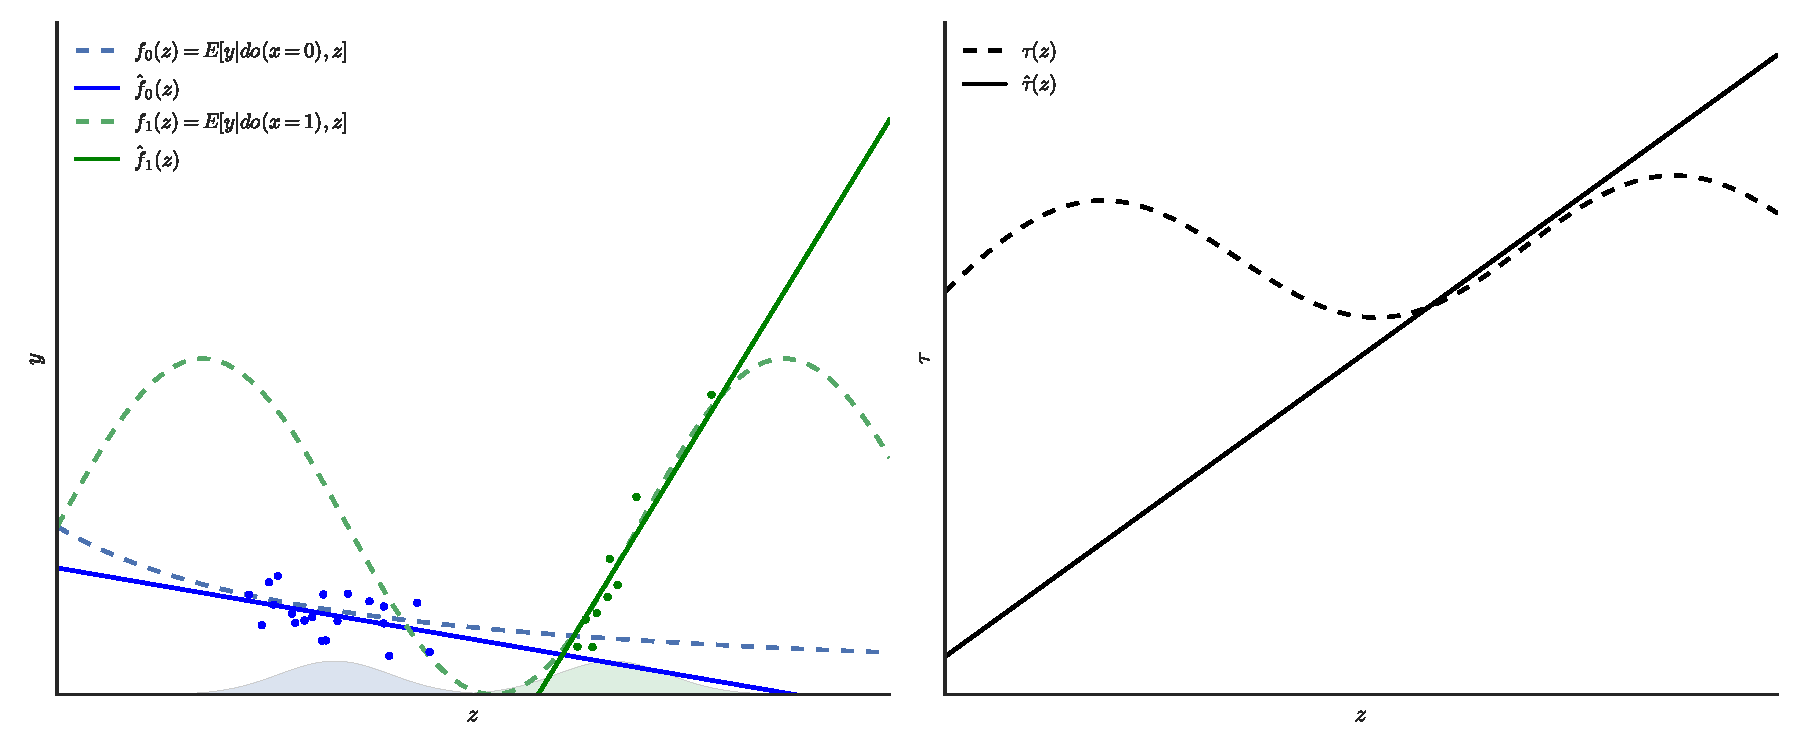
\includegraphics[scale=.55]{covariate_shift_estimation.pdf}
\end{figure}


A general approach to estimating the expectation of some function $f(\cdot)$ with respect to data from some distribution $\P{\cdot}$, when we have data sampled from a different distribution $\Q{\cdot}$ is importance sampling \citep{horvitz1952generalization,Koller2009}. 
\eqn{
\label{eqn:importance_sampling}
\Esub{\vb{v} \sim \P{\vb{v}}}{f(v)} = \Esub{\vb{v} \sim \Q{\vb{v}}}{f(v)\frac{\P{\vb{v}}}{\Q{\vb{v}}}}
}

This importance weighting approach can be applied to the covariate shift/average causal effect problem by weighting the terms in the empirical risk minimisation estimator \citep{Sugiyama2007}.

\eqn{
\label{eqn:importance_weighted_erm}
\hat{\theta}_{iw} &= \argmin_{\theta \in \Theta}\left[\frac{1}{n}\sum_{i=1}^n \ind{x_i=1} L\left(h_1(z_i;\theta),y_i\right)\frac{\P{z_i}\delta(x_i-1)}{\P{z_i}\P{x_i=1|z_i}}  \right] \\
&= \argmin_{\theta \in \Theta}\left[\frac{1}{n}\sum_{i=1}^n \ind{x_i=1} L\left(h_1(z_i;\theta),y_i\right)\frac{1}{e(z_i)}  \right],
}

where $e(\vb{z})$ is the propensity score, defined by \citep{Rosenbaum1983};
\eqn{
e(\vb{z})\equiv \P{x=1|\vb{z}}
}

The estimator in equation \ref{eqn:importance_weighted_erm} is an example of a doubly robust estimator \citep{scharfstein1999adjusting,}. Doubly robust methods are asymptotically unbiased as long as either the regression model $h$ or propensity score $e$ are correctly specified \citep{robins1995semiparametric}. 

The propensity score can be used to estimate the average causal effect without specifying a regression model for $\E{Y|X,\vb{Z}}$. \citet{Rosenbaum1983} demonstrated that if the ignorability assumption is satisfied by conditioning on $\vb{Z}$, then it is also satisfied by conditioning on $e(\vb{z})$. This allows for estimators based on stratifying, matching or regression on the propensity score rather than the covariates $\vb{Z}$. Inverse propensity weighting can also be combined with empirical estimation of $\E{Y|X,Z}$ yielding the simple, albeit inefficient, estimator in equation \ref{eqn:simple_inverse_propensity} \citep{Imbens2004}. In some settings, such as stratified randomised trials \citep{imbens2015causal} or learning from logged bandit feedback \citep{Bottou2013} the propensity score may be known. However in general, it must be estimated from data. Frequently this is done with a simple parametric model such as logistic regression, but a wide range of standard machine learning algorithms including bagging and boosting, random forests and nueral networks can also be applied   \citep{Austin2011}. \citet{Lunceford2004} review the theoretical properties of key propensity score based estimators, including stratification and inverse propensity weighting. 

\eqn{
\E{Y|do(X=x)} = \Esub{z\sim \P{\vb{Z}}}{\E{Y|x,\vb{z}}} = \Esub{z\sim \P{\vb{Z|x}}}{\E{Y|x,\vb{z}}\frac{1}{e(\vb{z})}}
}

\eqn{
\label{eqn:simple_inverse_propensity}
\hat{\tau}_{ip} = \frac{1}{n}\sum_{i=1}^n \left(\frac{\ind{x_i=1}y_i}{e(\vb{z}_i)} -\frac{\ind{x_i=0}y_i}{1-e(\vb{z}_i)}\right)
}


\subsubsection{Matching}
There is a straightforward connection between matching and regression for causal effect estimation. If $h \in \mathcal{H} \implies h + a \in \mathcal{H}$ for any constant $a$ and $\hat{f}$ is selected by minimising empirical risk with an $L_2$ loss then $\frac{1}{n}\sum_{i=1}^n \ind{x_i=1}\hat{f}_1(z_i) = \frac{1}{n}\sum_{i=1}^n \ind{x_i=1}y_i$ \footnote{\citep{Imbens2004} state this holds for most implementations}, and equation \ref{eqn:cef_empirical_regression} can be re-written as: 

\eqn{
\label{eqn:cef_regression_missing}
\hat{\tau}_{reg} = \sum_{i=1}^n \left[\ind{x_i=1}\left(y_i - \hat{f}_0(z_i)\right) +\ind{x_i=0}\left(\hat{f}_1(z_i) - y_i \right)\right]
}

This formulation of the regression estimator highlights the missing data aspect of casual effect estimation. For each instance, the regression models are used to estimate the counterfactual outcome had the instance received the alternate treatment. Matching estimates the counterfactual outcome for an instance from the outcome of \emph{similar} instances that received a different treatment. \citet{abadie2002simple} analyse an estimator where both target and control instances are matched and the matching is done with replacement, let $j \in J_k(i)$ be the indices of the $k$ instances closest to $i$ by some metric $d(z_i,z_j)$ such that $x_i \neq x_j$.

\eqn{
\hat{\tau}_{match} = \sum_{i=1}^n \left[\ind{x_i=1}\left(y_i - \frac{1}{k}\sum_{j \in J_k(i)}y_j\right) +\ind{x_i=0}\left(\frac{1}{k}\sum_{j \in J_k(i)}y_j - y_i \right)\right]
}

This estimator is equivalent to equation \ref{eqn:cef_regression_missing} with k nearest neighbour regression. There are many variants of matching estimators utilising different distance metrics, matching with or without replacement (and in the latter case, greedy or optimal matching) and with or without discarding matches beyond some threshold \citep{cochran1973controlling,rosenbaum1985constructing}. Although intuitive, matching estimators in general have poor large sample properties \citep{Abadie2006}. An exception is where the goal is to estimate the average treatment effect of treatment on the treated in settings where there is a large set of control instances (compared to treatment instances) \citep{Imbens2004}. 

The practical performance of the estimation approaches discussed in this section will depend on the sample size, dimensionality of the covariates, the complexity of the treatment assignment mechanism and output function, and the degree of prior knowledge available about these functions. A key difference between standard machine learning problems and causal effect estimation is that when estimating causal effects we cannot directly apply cross-validation or a hold-out set for model selection because we lack samples from the counterfactual. 

The significance of this should not be underestimated. Cross-validation has allowed applied machine learning to succeed with a very atheoretical approach on the basis that we can identify when a model is successful. With causal effect estimation there is no guarantee that a model that performs well at prediction (even out of sample) will accurately estimate the outcome of an intervention. \citet{Sugiyama2007} propose inverse propensity weighted cross validation for the covariate shift problem. There is relatively little theory on model selection for estimating the propensity score. To achieve asymptotically unbiased estimates, the covariates should satisfy the backdoor criterion. It is also known that conditioning on instrumental variables, which directly influence $X$ but not $Y$, increases variance without any reduction in bias and can increase bias if there are unmeasured confounding variables \citep{Wooldridge2009,Bhattacharya2012,Pearl2012b,Myers2011}. With doubly robust estimators, one could apply an iterative approach, fitting a propensity score model, using the results for inverse propensity weighted cross-validation of the regression model and then selecting covariates for the propensity model on the assumption the estimated regression function was correct. I have found no examples of such an approach.

The performance of methods for causal effect estimation can be tested on simulated data \citep{Frolich2001,zhao2004using,Hill2011,Dorie2016} or by comparing estimates from observational studies with the results from corresponding exeriments \citep{lalonde1986evaluating,Fraker1987,heckman1997matching,heckman1998characterizing,dehejia1999causal,Smith2001,Anglemyer2014}. Unfortunately there are a relatively small number of examples where comparable observational and experimental data are available. The results are mixed with later studies finding generally better alignment of results but it is hard to ascertain if this is due to improved methodological approaches or over-fitting to the available data-sets.  


\section{Causal Discovery}

%Cyclic models \cite{Hyttinen2012}

We now move to the much more general problem of learning a causal graph from observational data. In this setting we make much broader assumptions about the structure of the graph. For example, that it is acyclic or that we have no unmeasured confounding variables. We do not assume the existence or directions of any links between the variables. Amazingly, it is possible to infer some aspects of causal structure with such general assumptions. The set of conditional independence in a non-experimental data set indicates some causal structures are more likely than others. In addition, there can be subtle asymmetries in the relationship between the joint distribution of cause and effect and the distributions of cause given effect and effect given cause. These clues are the key to causal discovery algorithms.

%There is also work on inferring causal structure from experiential data \ref{}. We discuss this further in section XXX.

Causal discovery is a much grander goal than causal effect estimation given a known causal network. Arguably, if achieved, it would equate to the automation of scientific discovery. We need simply supply our algorithm with a vast collection of variables (regardless of their relevance to the problem) and it would learn the causal structure and from that allow us to estimate the effects of any intervention we cared to make. Unfortunately, causal discovery is very hard. Even with the assumption that the causal graph is acyclic and there are no latent variables, the number of possible graphs grows exponentially with the square of the number of variables .

% - some intuition here about the strength of the signal we get from causal discovery. Small initial errors in greedy approaches can cascade leading to unstable inference and large losses \ref{sprites?}. Talk about the numerical as well as the statistical issues here. 

In the next sections we briefly survey the key approaches to causal discovery. We roughly divide the methods into those based on those that exploit the connection between the conditional independencies in a joint distribution and the structure of a causal model and those that leverage assumptions about the functional form of the relationships between cause and effect. 

%This is not the only way we could have grouped them. There is also a separation between constraint based algorithms, that XXXX and those that search and score multiple graph structures before selecting the best. There are also hybrid methods \ref{}  

\subsection{Conditional independence based methods}
One general approach is to look for clues about the structure of the network in the conditional independence relations in the distribution. For any Bayesian network, $G$, (causal or not) we can read of conditional independencies in the joint distribution from the structure of the network. If a set of variables $Z$ d-separates $X$ and $Y$ in $G$ then $(X \ci Y|Z)$ in the distribution $P$. However, we want to work in the other direction, from conditional independence in the distribution to the structure of the network. This requires that we assume the reverse condition: $(X \ci Y|Z)$ in $P$ must imply $Z$ d-separates $X$ and $Y$ in $G$. This assumption, commonly referred to as  \textbf{\textit{faithfulness}} \ref{Sprites2000}, says there are no additional independence relations that are satisfied in $P$ but not in all distributions $\boldsymbol{P'}$ that are compatible with $G$. Stating that $P$ is faithful to $G$ is equivalent to $G$ is a \textbf{\textit{perfect map}} \cite{pearl1988probabilistic} for $P$.

Faithfulness is an assumption. It does not always hold and we cannot verify it from the observational data we wish to use for causal inference. However, most distributions generated by a causal Bayesian network will be faithful to that network. For faithfulness to be violated, different causal effects must exactly balance one-another out. For example, consider a simple binary variable model of chocolate consumption, income and obesity (figure). If the coefficients in the conditional probability tables are just right then the direct effect of chocolate on obesity will exactly balance the indirect effect through income and obesity will appear independent of chocolate consumption. However, this independence is not stable. It would disappear under a small perturbation to any of the parameters. In discrete systems, violations correspond to the solutions to polynomial equations over values in the CPD tables and thus are a space of measure zero with respect to all possible distributions associated with the graph \citep{Koller2009}. 

Given the faithfulness assumption, our causal discovery problem reduces to finding the set of Bayesian networks that have exactly the dependency structure as we observe in $P$. This set can also be referred to as the Markov equivalence class compatible with $P$.

\subsubsection{Without hidden common causes}
The strong assumption that there are no hidden variables that cause two or more variables in $\boldsymbol{V}$ significantly reduces the 'search space' of Bayesian networks we must consider. This assumption is referred to as causal sufficiency \citep{Sprites2000}.

We will begin with a brute force algorithm (described as the SGS algorithm in \citet{Sprites2000} and IC algorithm in \citet{Pearl2000}). While it is impractical for all but the smallest of networks, it demonstrates key concepts that also underlie the more useful and complex algorithms we will discuss later. 

\begin{table}[H]
 \begin{tabularx}{\textwidth}{X}
 \hline
\rule{0pt}{2.5ex} 
 \textbf{The SGS (or IC) Algorithm}\\
 \hline
 \rule{0pt}{2.5ex}
\textbf{Input:} A distribution $P$, over variables $\boldsymbol{V}$, that was generated by and is faithful to an (unknown) Bayesian network $G$\\
\textbf{Output:} A partially directed network that represents the Markov equivalence class of $G$\\
 \begin{enumerate}[itemsep=8pt]
  \item Join all pairs of vertices $(a,b) \in \boldsymbol{V}$ with an un-directed link to form a complete graph.
  \item For each link $a-b$ search for a set $\boldsymbol{S}_{a,b} \subseteq V \setminus \{a,b\}$ that renders $a$ and $b$ conditionally independent. If such a set (including the empty set) exists then $a$ and $b$ cannot be directly connected in $G$ so delete the link.
  \label{alg:SGSexponential}
  
  \item For all pairs of non-linked variables $(\alpha,\beta)$ with a common neighbour, $c$, if $c \notin \boldsymbol{S}_{\alpha,\beta}$, then $c$ must be a collider in the path $\alpha,c,\beta$ so  add arrows to direct the links $\alpha-c$ and $\beta-c$ towards $c$.
  \label{alg:SGScolliders}  
  \item Recursively try to orient any edges that remain un-directed to avoid creating cycles (because they are not there by assumption) and additional colliders (because any colliders were found in step \ref{alg:SGScolliders}).
  \label{alg:SGSfinal}
\end{enumerate}\\
 \hline
\end{tabularx}
\end{table}

The SGS algorithm utilises the fact that a collider structure (figure \ref{fig:dseptripple4}) induces a distinct conditional independence relation. Assuming you have a consistent conditional independence test, it converges to return a partially directed network that represents the Markov equivalence class for the generating causal model. Unfortunately the number of conditional independence tests required for step \ref{alg:SGSexponential} grows exponentially (in the worst case) with the number of variables. Not only that, but for each edge that is in the true network, the algorithm will always tests all other possible subsets of variables. If the assumption that there are no hidden common causes or that the distribution is faithful are violated, step \ref{alg:SGScolliders} of the SGS algorithm can produce double headed arrows.

The PC algorithm \citet{Sprites2000} modifies step \ref{alg:SGSexponential} of the SGS algorithm to utilise the fact that if two variables $(a,b)$ are conditionally independent given some set, they will also be conditionally independent given a set that contains only variables adjacent to $a$ or $b$. It also checks for low order conditional independence relations before higher order ones. This allows it to exploit any sparsity in the true network, leading to much better average case performance  \citep{Sprites2000} (although the worst case, where the true network is complete, is still exponential). With finite data, the order in which the links are considered can change the output (unlike for SGS). The effect of wrongly removing a link early on flows through to later conditional independence tests by changing which nodes are considered adjacent.

\begin{table}[H]
 \begin{tabularx}{\textwidth}{X}
 \hline
\rule{0pt}{2.5ex} 
 \textbf{The PC Algorithm}\\
 \hline
 \rule{0pt}{2.5ex}
\textbf{Input:} A distribution $P$, over variables $\boldsymbol{V} = \{V_{1}...V_{k}\}$, that was generated by and is faithful to an (unknown) Bayesian network $G$\\
\textbf{Output:} A partially directed network that represents the Markov equivalence class of $G$\\
 \begin{enumerate}[itemsep=8pt]
  \item As for SGS
  \item \textbf{for} each link $a-b$:
  \begin{itemize}[label={}]
   \item $n = 0$
   \item $\boldsymbol{A}_{a,b} = \{A_{1}...A_{j}\}$ be the set of nodes adjacent to $a$ and/or $b$
   \item \textbf{while} $a$ and $b$ are connected and $n < j$:
   \item 
    	\begin{itemize}[label={}]
    	\item \textbf{if} any subset of size $n$ of $\boldsymbol{A}$ makes $a$ and $b$ conditionally independent:
    	\item \begin{itemize}[label={}]
    			delete the link
    		  \end{itemize}
    	
    	\item $n = n+1$
    	\end{itemize}
  \end{itemize}   
  \item as for SGS
  \item as for SGS
\end{enumerate}\\
 \hline
\end{tabularx}
\end{table}

The PC algorithm also returns a set of Markov equivalent networks consistent with the distribution. Since we have assumed there are no hidden variables, for any single graph in this set we can calculate causal effects from the truncated product formula \ref{eq:truncatedproduct}. We can then bound the true causal effect by combining the results for the all the networks. This procedure is the IDA algorithm \citep{Maathuis2009} and has been found to outperform standard regularisation techniques at finding causal effects in a high-dimensional yeast gene expression data set \citep{Maathuis2010}. An implementation is available in the R package \citep{Kalisch2012} 

\subsubsection{With hidden variables}
There are an number of difficulties in extending the approach of the last section to deal with the case where there are latent variables. With an unknown number of hidden variables there are infinity many possible structures to search over. In addition, the space of causal networks is not closed under marginalisation. If we have a distribution that $P'(\boldsymbol{O},\boldsymbol{U})$ generated by and is faithful to a network $G$ the distribution $P(\boldsymbol{O})$, that results from marginalising over $\boldsymbol{U}$, may not be faithful to any Bayesian network (see figure \ref{fig:DAGSnotclosed}). The key to constraining the space of possible models is that many latent structures are equivalent (under transforms of the hidden variables).

\begin{figure}
\centering
\caption{A distribution faithful to this DAG is not faithful to any DAG over the variables $\{A,B,C,D\}$ after marginalising over $U$. }
\label{fig:DAGSnotclosed}
 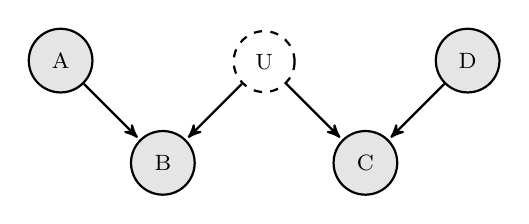
\begin{tikzpicture}[->,>=stealth',shorten >=1pt,auto,node distance=1cm,  thick,main node/.style={observed},lt/.style={latent}]
 %nodes
\node[lt](1){U}; 
\node[main node, below left = of 1](2){B};
\node[main node, below right = of 1](3){C};
\node[main node, above left= of 2](4){A};
\node[main node, above right = of 3](5){D};

 \path[every node/.style={font=\sffamily\small}]
    (1) edge node {} (2)
    	edge node {} (3)
    (4) edge node {} (2)
    (5) edge node {} (3);
    	
\end{tikzpicture}
\end{figure}
 
\begin{theorem}
\cite{Verma1993} For every latent structure there is a dependency equivalent structure such that every latent (unobserved) variable is a root node with exactly two children .
\end{theorem}

Since we only care about the causal relationships between observed variables, it is sufficient to search over networks where any hidden variables have no parents and directly cause two of the observed variables. Instead of representing hidden variables explicitly we can capture the necessary independence relations with a more general graphical model that supports bi-directed edges that play the role of a hidden confounding variable. These models, referred to as maximal ancestral graphs (MAGs) are closed under marginalisation and conditioning. 

For any DAG with latent (and selection) variables there is a unique MAG \cite{Richardson2002}. This makes it possible to extend the PC algorithm to latent structures, resulting in the FCI algorithm \cite{Sprites}. The logic behind the algorithm is very similar. Certain structures are ruled out as a consequence of being inconstant with the observed conditional independence relations. The output is an equivalence class of MAGs, which can be represented graphically as a partial ancestral graph PAG \cite{Spirtes1995}. Assuming there are no selection variables, the PAG can contain four types of link:

\begin{enumerate}
\item $X \rightarrow Y$, meaning $X$ causes $Y$
\item $X \leftrightarrow Y$, meaning there is a latent variable that causes $X$ and $Y$.
\item $X\ {\circ} {\rightarrow}\ Y$, either $X$ causes $Y$ or a latent variable causes both.
\item $X\ {\circ} {-}  {\circ}\ Y$, either $X$ causes $Y$ or $Y$ causes $X$ or a latent variable causes both.
\end{enumerate}

The circles indicate where it is ambiguous if there should be an arrowhead (IE where there is one in some MAGs and not in others in the equivalence class). Counter-intuitively it is sometimes possible to  rule out or confirm the existence of a confounding variable and fully determine the causal type of a link (see examples in figure \ref{fig:FCIExamples}). 


\begin{figure}
\centering
\caption{FCI examples: true graph and FCI output}
\label{fig:FCIExamples}
 \begin{subfigure}[t]{0.4\textwidth}
 \centering
 \caption{True DAG}
 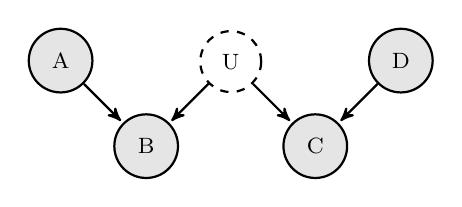
\begin{tikzpicture}[->,>=stealth',shorten >=1pt,auto,node distance=.7cm,  thick,main node/.style={observed},lt/.style={latent}]
 %nodes
\node[lt](1){U}; 
\node[main node, below left = of 1](2){B};
\node[main node, below right = of 1](3){C};
\node[main node, above left= of 2](4){A};
\node[main node, above right = of 3](5){D};

 \path[every node/.style={font=\sffamily\small}]
    (1) edge node {} (2)
    	edge node {} (3)
    (4) edge node {} (2)
    (5) edge node {} (3);
    	
\end{tikzpicture}
 \end{subfigure}
 \begin{subfigure}[t]{0.4\textwidth}
  \centering
  \caption{Partial ancestral graph}
 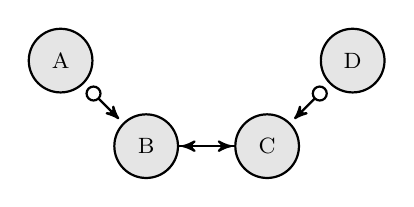
\begin{tikzpicture}[->,>=stealth',shorten >=1pt,auto,node distance=.7cm,  thick,main node/.style={observed}]
 %nodes

\node[main node](1){A};
\node[main node, below right=of 1](2){B};
\node[main node, right=of 2](3){C};
\node[main node, above right=of 3](4){D};

 \path[every node/.style={font=\sffamily\small}]
    (1) edge[pil] node {} (2)
    (2) edge node {} (3)
    (3) edge node {} (2)
    (4) edge [pil] node {} (3);    	
\end{tikzpicture}
\end{subfigure}
\par\bigskip 
 \begin{subfigure}[t]{0.4\textwidth}
 \centering
 \caption{True DAG}
 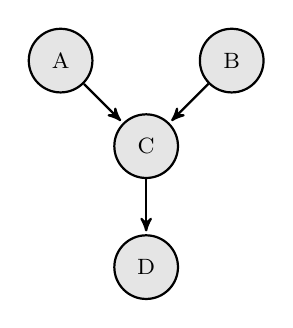
\begin{tikzpicture}[->,>=stealth',shorten >=1pt,auto,node distance=0.7cm, thick,main node/.style={observed},lt/.style={latent}]
 %nodes

\node[main node](1){C};
\node[main node, above left=of 1](2){A};
\node[main node, above right=of 1](3){B};
\node[main node, below=of 1](4){D};

 \path[every node/.style={font=\sffamily\small}]
    (1) edge node {} (4)
    (2) edge node {} (1)
    (3) edge node {} (1);    	
\end{tikzpicture}
\end{subfigure}
 \begin{subfigure}[t]{0.4\textwidth}
  \centering
  \caption{Partial ancestral graph}
 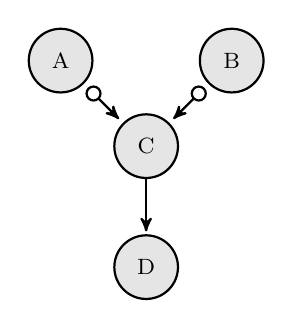
\begin{tikzpicture}[->,>=stealth',shorten >=1pt,auto,node distance=0.7cm,  thick,main node/.style={observed}]
 %nodes

\node[main node](1){C};
\node[main node, above left=of 1](2){A};
\node[main node, above right=of 1](3){B};
\node[main node, below=of 1](4){D};

 \path[every node/.style={font=\sffamily\small}]
 	(1) edge node {} (4)
    (2) edge [pil] node {} (1)
    (3) edge [pil] node {} (1);    	
\end{tikzpicture}
\end{subfigure}
\end{figure} 

The FCI algorithm can be made complete such that it discovers all aspects of the true causal structure that are identifiable from the conditional independence relations of a distribution over observed variables and the faithfulness assumption \cite{Zhang2008}. More recently \cite{Colombo2012} have proposed the RFCI algorithm, which in some cases returns more ambiguous links than FCI but is substantially faster. \cite{Claassen2013} point out that the problem of learning sparse causal networks from data is not NP-hard and propose the FCI+ algorithm, that requires $O(N^{2(k+2)})$ conditional independence tests, where $k$ is the maximum node degree over the observed variables. 

Latent variables can create constraints on the marginal distribution over the observed variables that cannot be expressed in term of conditional independencies. These generalised constraints can be expressed and leveraged within nested Markov models \citep{Richardson2012,Shipster2014} 


%\renewcommand{\arraystretch}{1.5}
%\begin{tabular}{| c | c | p{4cm} | c | c | c |}
%\hline
%  \textbf {Alg.} &\textbf{ Method }& \textbf{Scales (num.vars) }& $\sim $ \textbf {Vars} & \textbf {Latent } & \textbf {Reference} \\
%  \hline
%  IC/SGS & Constraint based & Exponential & 10 & No & Pearl(2000)/Sprites(2000)\\
%  \hline
%  PC & Constraint based & Worst case exponential, polynomial for sparse graphs & 5000 & No & Sprites(2000) \\ 
%  \hline
%  FCI & Constraint based & Worst case exponential, polynomial variant FCI+ for sparse graphs & 30 & Yes & Sprites(2000) \\
%  \hline
%  RFCI & Constraint based & ? & 500 & Yes & Colombo(2012) \\
%  \hline
%  GES & Search \& Score  & Worst case exponential & 50 & No & Chickering(2002) \\
%  \hline
%  MMHC & Hybrid & ? & 5000 & No & Tsamardinos(2006) \\
% \hline
%\end{tabular}

All the algorithms discussed in this section rely on being able to perform conditional independence tests. This is non-trivial with high dimensional data. If the functional relationship between the variables is linear with Gaussian noise then the network represents a multivariate normal distribution and a pair of variables are conditionally independent if and only if the corresponding entry in the inverse correlation matrix is non-zero \citep{Koller2009}. Where the functions are non-linear one can apply kernelised independence tests \citep{Gretton2008,Zhang2012}


\subsection{Discovery with functional models}
The algorithms we have considered so far return a Markov equivalence class. They cannot distinguish between two models that result in the same set of conditional independence relations. Consider the very simple case where  there are only two variables and the possible causal structures are $X \rightarrow Y$ or $Y \rightarrow X$. These models have the same dependency structure but in one case $P(Y|do(X)) = P(Y|X)$ and in the other $P(Y|do(X)) = P(Y)$. No algorithm relying purely on conditional independence relations can separate these two cases. 

Let us focus only on the two variable case $X \rightarrow Y$ or $Y \rightarrow X$. What possible clues could there be in the distribution $P(X,Y)$ that could indicate which causal model it was generated from? Recall the functional definition of causality (section \ref{sec:SEM}). There are a number of assumptions about the form of the functions that can allow us to identify the causal direction: non-invertable functions, additive noise \cite{Hoyer2009}, post-non-linear additive noise \cite{Zhang2008a} or linear models with non-Gaussian noise \cite{Hoyer2012}.

The causal direction can also be identified via a connection between casual discovery and semi-supervised learning \citep{Janzing2012}. Suppose we are trying to learn $\P{Y|X}$. The goal of semi-supervised learning is to improve our estimate of $\P{Y|X}$ by leveraging additional data sampled from $\P{X}$. However, if the true causal model is $X \rightarrow Y$ then their is some function mapping values of $X$ to $Y$ which should be invariant to any changes in the input distribution $\P{X}$. Therefor $\P{X}$ should be independent of $\P{Y|X}$ and semi-supervised learning should not perform any better than standard supervised learning. However if the true causal model is $Y \rightarrow X$ then variations in the $\P{X}$ can result from both the input distribution over $Y$ and the mapping from $X$ to $Y$ and semi-supervised learning could help. This assumption of independence of mechanism and input can also allow the identification of the causal direction in SEMs even where the functions are deterministic and invertable \citep{Daniusis2010}. \citet{Janzing2012a} leverage an information geometric viewpoint of the independence of mechanism and input to infer the causal direction between a pair of associated variables.  

Instead of positing a functional restriction on the relationship between variables and then developing theory to exploit that assumption, \citep{LopezPaz2014} propose learning what the causal relationship looks like from data. They assume there will be a difference between the relationship of $\P{X}$, $\P{Y}$ and $\P{X|Y}$ between $X \rightarrow Y$ versus $Y \rightarrow X$. Their algorithm requires a data set in which each row is itself a data set consisting of pairs of variables $(x_i,y_i)$ with a label indicating the direction of causality between $X$ and $Y$. They use a kernel mean embedding to represent the distributions $\P{X}$, $\P{Y}$ and $\P{X|Y}$ as features for each individual sub-data set and train an algorithm to learn the direction of causality. Unfortunately we do not have a large collection of data sets where the causal direction is known to train such a model. \citet{LopezPaz2014} instead use a simulated data set so their model will necessarily be based on the assumptions they make when generating the data. Nonetheless this approach makes it possible to rapidly construct a model from a wide range of possible assumptions, without doing a lot of theory to design a specific algorithm optimised to that setting. 

\citep{Peters2014} have extended results from the bi-variate case to the multivariate setting. They show that if we can come up with a condition that guarantees identifiability for the bi-variate case, we can extend that result to get the conditions under which the multivariate case is identifiable. They build on this to develop an algorithm that allows the construction of causal graphs based on the additive noise assumption. 

\chapter{The interventionist viewpoint}

The previous sections all focus on aspects of the question; how can we estimate the effect of an intervention in a system from data collected prior to taking it. There is an obvious alternative. Instead of trying to infer the outcome of an intervention from passive observations one can intervene and see what happens. There are three key differences between observing a system and explicitly intervening in it. Firstly, when we intervene we choose which actions to take and thus have control over which data points we obtain to learn from. Selecting data points optimally for learning is the focus of the optimal experimental design liturature within statistics \citep{pukelsheim2006optimal} and the active learning liturature in machine learning \citep{settles2010active}. Secondly, explicitly choosing interventions yields a perfect model of the probability with which each action is selected, given any context, allowing control over confounding bias. Finally, when we are intervening in a system we typically care about the impact of our actions on the system in addition to optimising learning. For example, in a drug trial , assigning people a sub-optimal treatment has real world costs. This leads to a trade-off between exploiting the best known action so far and exploring alternative actions about which we are less certain. This exploration-exploitation trade-off lies at the heart of the field of reinforcement learning \citep{sutton1998reinforcement}. 

\section{Randomised experiments}
Randomised controlled trials are often presented as the gold standard for determining causal effects. What is it about randomisation that makes it so important when it comes to causality? The graphical model for a randomised controlled experiment is shown in figure \ref{fig:random_experiment_network}. If we assume perfect compliance (everyone takes the treatment that we select for them) then we have a perfect model for the treatment assignment process. Since treatment is assigned randomly, there can be no other variables that influence it and thus no confounding variables that effect both treatment and outcome. 

\begin{figure}
\caption{causal network for a randomised experiment}
\label{fig:random_experiment_network}
\centering
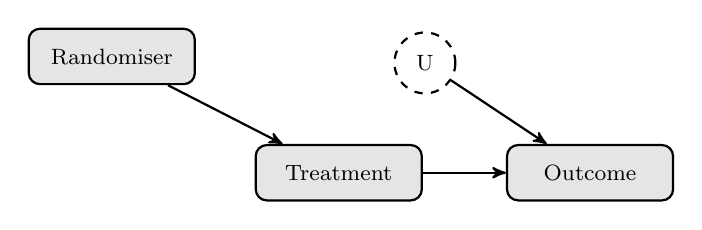
\begin{tikzpicture}[->,shorten >=0pt,shorten <=0pt,node distance=3em,thick, node/.style={observedrect}, lt/.style={latent}]
\node[node](1){Treatment};
\node[node, above left=of 1](2){Randomiser};
\node[node, right=of 1](3){Outcome};
\node[lt, above left=of 3](4){U};
\path[]
	(2) edge (1)
	(1) edge (3)
	(4) edge (3);
\end{tikzpicture}
\end{figure} 

Randomisation does not ensure target and control group are exactly alike. The more other features (observed or latent) influence the outcome, the more likely it is that there will be a significant difference in the joint distribution of these variables in a between the target and control groups in a finite data sample. However, the variance in the outcome within both the target and control groups also increases. The net result is increased variance (but not bias) in  the estimate of causal effects. 

Stratified randomised experiments address the issue of variance due to covariate imbalance by randomly allocating treatment conditional on covariates belived to influence the outcome of interest. This introduces a backdoor path from treatment to outcome via the covariates on which treatment is stratified, see figure \ref{fig:random_experiment_network_stratified}, nessessitating that one condition on these covariates in computing the average casual effect in the same way as for estimating causal effects under under ignorability \S\ref{sec:causal_effect_under_ignorability}. The key difference is that the propensity score is known, as it is designed by the experimenter, and there are guaranteed (rather than assumed) to be no latent confounding variables (that influence both treatment and outcome). See \citet{imbens2015causal} for a discussion of the trade-offs between statified versus completely random experiments. 

\begin{figure}
\caption{causal network for a stratified randomised experiment}
\label{fig:random_experiment_network_stratified}
\centering
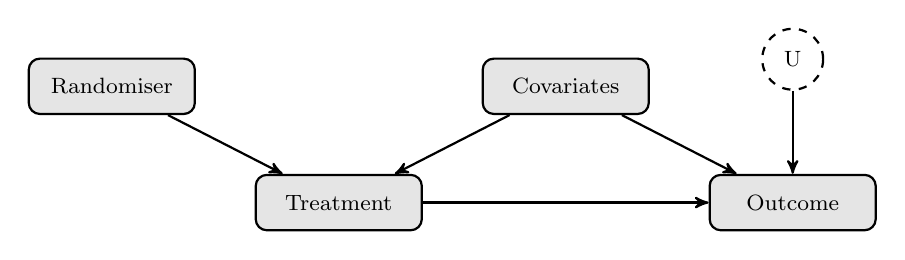
\begin{tikzpicture}[->,shorten >=0pt,shorten <=0pt,node distance=3em,thick, node/.style={observedrect}, lt/.style={latent}]
\node[node](1){Treatment};
\node[node, above left=of 1](2){Randomiser};
\node[node, above right=of 1](5){Covariates};
\node[node, below right=of 5](3){Outcome};
\node[lt, above=of 3](4){U};

\path[]
	(2) edge (1)
	(1) edge (3)
	(4) edge (3)
	(5) edge (3) edge (1);
\end{tikzpicture}
\end{figure} 

The benefit provided by randomisation in breaking the link between the treatment variable and any latent confounders should not be understated. The possibility of unobserved confounders cannot be empirically ruled out from observational data \citep{Pearl2000} (there is no test for confounding). This means causal estimates from non-experimental data are always subject to the criticism that an important confounder may have been overlooked or not properly adjusted for. However, randomised experiments do have some limitations. 

\subsection{Limitations of randomised experiments}
\label{subsec:limitations_of_experiment}

The idealised notion of an experiment represented by figure \ref{fig:random_experiment_network} does not capture the complexities of randomised experiments in practice. There may be imperfect compliance, the treatment selected by the randomiser is not always followed, or output censoring, the experimenter is not able to observe the outcome for all units (for example if people drop out). If compliance or attrition is not random but associated with (potentially latent) variables that also effect the outcome then the problem of confounding bias returns.\footnote{Non-compliance is a problem if the goal is to estimate the causal effect of the treatment on the outcome but not if the goal is to estimate the causal effect of prescribing the treatment. The latter makes sense in a context where the process by which people decide whether or not to take the treatment they have been prescribed is likely to be the same if the treatment were made available more generally beyond experimental trial.} See figure \ref{fig:random_experiment_network_imperfect_compliance} for a the graphical model of a randomised experiment with imperfect compliance.

\begin{figure}
\caption{causal network for a randomised experiment with imperfect compliance}
\label{fig:random_experiment_network_imperfect_compliance}
\centering
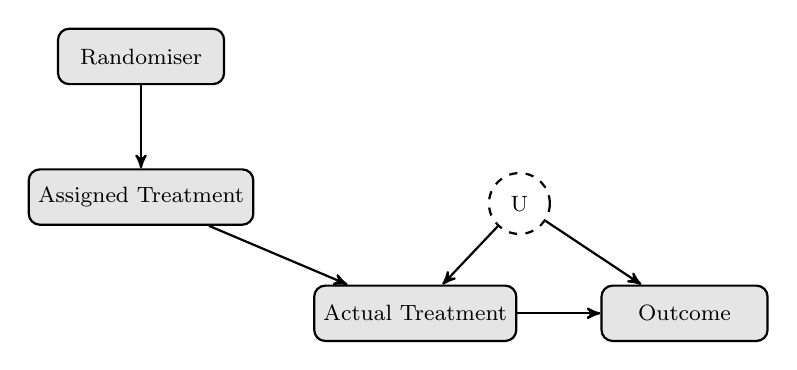
\begin{tikzpicture}[->,shorten >=0pt,shorten <=0pt,node distance=3em,thick, node/.style={observedrect}, lt/.style={latent}]
\node[node](1){Actual Treatment};
\node[node,above left=of 1](5){Assigned Treatment};
\node[node, above =of 5](2){Randomiser};
\node[node, right=of 1](3){Outcome};
\node[lt, above left=of 3](4){U};
\path[]
	(2) edge (5)
	(5) edge (1)
	(1) edge (3)
	(4) edge (3) edge (1);
\end{tikzpicture}
\end{figure} 

It is not always possible or ethical to conduct a randomized controlled trial as is beautifully demonstrated by the paper of \citet{smith2003parachute} on randomised cross-over trials of parashute use for the reduction of the mortality and morbity associated with falls from large hights \ref{fig:parashute}. When experimentation is possible, it is frequently difficult or expensive. This means experimental data sets are often much smaller than observational ones, limiting the complexity of models we can explore. In addition, they are often conducted on a convenient but unrepresentative sample of the broader population of interest (for example first year students at research universities). This can result in estimates with high \emph{internal validity} \citep{Campbell1963} in that they should replicate well in a similar population, but very low \emph{external validity}; the results may not carry over to the general population of interest. The question of whether an experiment conducted on one population can be mapped to another is referred to as the transportability problem \citep{Bareinboim2013} and relies on very similar assumptions and arguments to causal inference and the do-calculus. 

\begin{figure}
\begin{center}
\caption{Experiments are not always ethical; an illustration of a randomised cross-over trial of parashutes for the prevention of morbitity and mortality associated with falls from large heights.}
\label{fig:parashute}
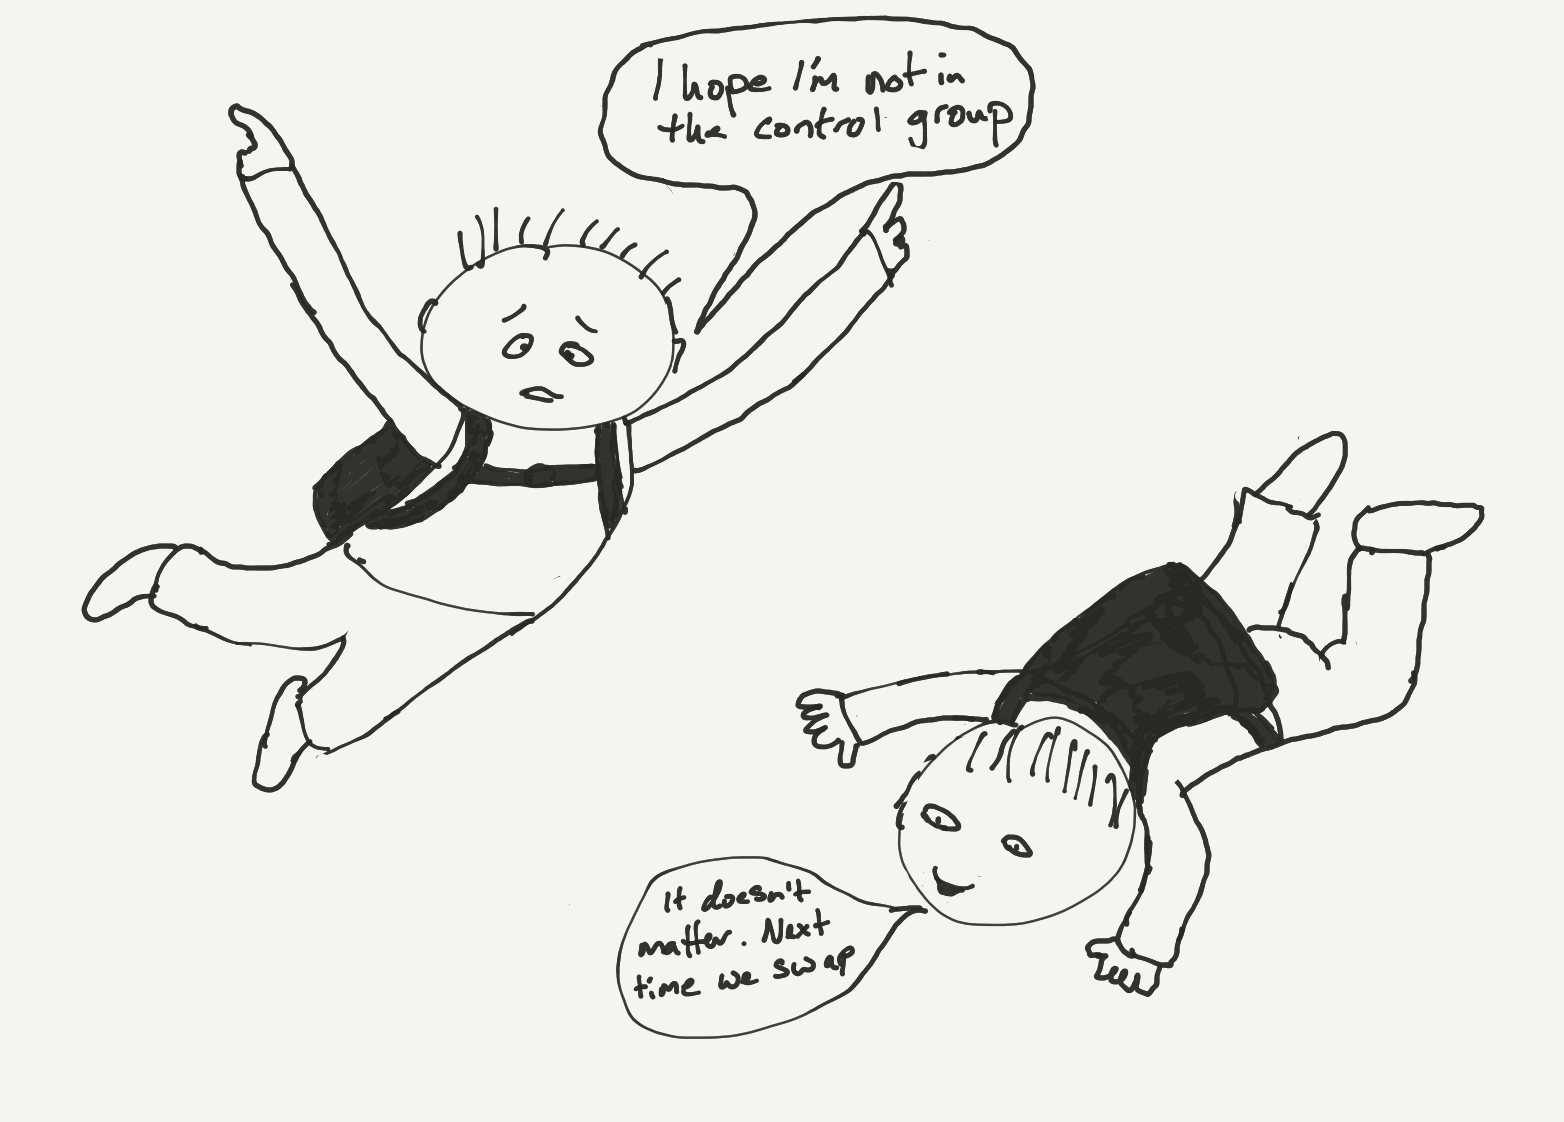
\includegraphics[scale=.4]{double_blind_parashute_trial_cartoon.png}
\end{center}
\end{figure}

Finally, non-adaptive randomised experiments are not optimal from either an active or reinforcement learning perspective. As an experiment proceeds information is obtained about the expectation and variance of each intervention (or treatment). Fixed experimental designs cannot make use of this information to select which intervention to try next. This results in both poorer estimates for a fixed number of experimental samples and more sub-optimal actions during the course of the experiment.

\section{Multi armed bandits}
\label{sec:multi-armed-bandits}

Multi-armed bandits address the problem of desiging experiments that can adapt as samples are observed. Their introduction is generally attributed to \citet{Thompson1993}. In its classic formulation \cite{Robbins1952,Lai1985} the (stochastic) k-armed bandit describes a sequential decision making problem, with $k$ possible actions or arms. Each arm $i$ is associated with a fixed but unknown reward distribution. \footnote{In order to quantify the performance of bandit algorithms, some assumptions are required on the distributions from which the rewards are generated. It sufficient (but not nessessary) to assume they are sub-Gaussian.} For each time step up to some horizon $T$ the learner selects an action and receives a reward, sampled i.i.d from the marginal distribution corresponding to that action. The goal of the learner is to maximise the total reward they receive. This problem captures the exploration-exploitation trade-off, the learner must balance playing arms that have yielded good results previously with exploring arms about which they are uncertain.

\vspace{0.5cm}
\begin{definition}[Stochasitic k-armed bandit problem]
Let $\actionspace = \set{1,...k}$ be the set of available actions (or bandit arms) and $\P{\vec{Y}} = \P{Y_1,...,Y_k}$ be the joint distribution over the rewards for each action. The multi-armed bandit problem proceeds over $T$ rounds. In each round $t$, 
\begin{enumerate}
\item the learner selects an action $a_{t} \in \set{1,...,k}$, based on the actions and rewards from previous time-steps and a (potentially stochastic) \emph{policy} $\pi$
\item the world stochastically generates the rewards for each action, $[Y_{t,1},...,Y_{t,k}] \sim \P{\vec{Y}}$
\item the learner observes and recieves (only) the reward for the selected action $Y_{t,a_t}$ 
\end{enumerate}
At the end of the game the total reward obtained by the learner is $\sum_{t=1}^T Y_{t,a_t}$. We denote the expected reward for the action $i$, $\E{ \P{Y_i}}$, by $\mu_i$ and the action with the highest expected reward by $i^*$. 
\end{definition} 

The total reward a bandit algorithm/policy can expect to acheive depends on the distributions from which the rewards for each action are sampled. To account for this, the performance of bandit algorithms is quantified by the the difference between the reward obtained by the algorithm and the reward that would have been obtained by an oracle that selects the arm with the highest expected reward at every time step. This difference is known as the (cummulative) regret \footnote{The term regret is somewhat overloaded in the reinforcement learning liturature. There are alternative definitions that arise in the related problems of adversarial bandits and learning from expert advice. In addition, researches often refer to the expected regret as \quotes{the regret}.},
\eqn{
\label{eqn:raw_regret}
\rawregret = \sum_{t=1}^T Y_{t,i^*} - \sum_{t=1}^T Y_{t,a_t}
}

Both the rewards and the actions selected by the algorithm are random variables. The majority of work in the bandit liturature focuses on analysing and optimising some form of the expected regret, however there has been some work that also considers the concentration of the regret \citep{Auer1995,Audibert2007,Audibert2009exploration}. The expectation of the regret, as defined by equation \ref{eqn:raw_regret}, is refered to as the pseudo-regret \citep{Bubeck2012} and is given by equation \ref{eqn:pseudo_regret}. A stochastic bandit algorithm is learning if it obtains psuedo-regret that is sub-linear in $T$. 

\vspace{0.5cm}
\begin{definition}[Pseudo-Regret]
\eqn{
\label{eqn:pseudo_regret}
\regret(\pi) &= \max_{i \in \set{1,...,k}}\E{\sum_{t=1}^T{Y_{t,i}}} - \E{\sum_{t=1}^T{Y_{t,a_t}}} \\
&= n\mu_{i^*} - \E{\sum_{t=1}^T{Y_{t,a_t}}}
}
\end{definition}

The regret is invariant to adding a constant to the expected rewards for all actions. However, it still depends on key characteristics of the reward distributions for each action. Bandit algorithms are designed given assumptions about the form of the distributions, such as that they come from a given family (i.e bernoulli bandits, gaussian bandits) or that the rewards are bounded in some range. Given these assumptions, the performance of the algorithm is characterised in two ways; by the \emph{problem dependent regret}, which typically depends on how far each arm is from optimal and by the \emph{worst case regret}, which is the maximum regret over all possible configurations of the reward distributions (for a given horizon $T$ and number of arms $k$).

\todo{consider mentioning Thompson sampling and Bayesian bandits} 

\subsection{Stochastic bandits: Approaches and results}

The adaptive nature of multi-armed bandit algorithms complicates the design and analyse of estimators. The action selected by an algorithm at a given timestep can depend on the history of previous actions and rewards. As a result, the probability that each action is selected evolves over time, the actions are not sampled i.i.d from a fixed distribution and the number of times each action is selected is a random variable. The expectation and variance guarentees of standard estimators do not hold in this setting, see figure \ref{fig:early_stopping} for a concrete example. This makes it very difficult to  obtain an analytical expression for the expected regret for a given algorithm and problem. Instead, the focus is on computing bounds on the expected regret. 

\begin{figure}[h]
\centering
\caption{Standard empirical estimators can be biased if the number of samples, $n$, is not fixed in advance, but is a random variable that depends on the values of previous samples. This example plots the distribution (over $10^6$ simulations) of $\hat{\mu} = \frac{1}{n}\sum_{i=1}^n X_i$, where $X_i \sim bernoulli(0.2)$. In each simulation, we stop taking samples if the average value of $X_i$ up to that point exceeds a threshold of $0.3$ or $n$ reaches $100$. $\E{\hat{\mu}} = 0.439$. The estimator is substantially biased above $\E{X_i} = 0.2$ by the early stopping. Note that excluding experiments that were stopped early creates a bias in the opposite direction, $\E{\hat{\mu}|n=100} = 0.185$, as trials that obtained positive results early are excluded. This has some interesting potential real world implications. Early stopping of clinical trials is controversial. A researcher conducting a meta-analysis who wished to avoid (rather than bound) bias due to early stopping would have to exclude not only those trials which were stopped early but those which \emph{could} have been stopped early.}
\label{fig:early_stopping}
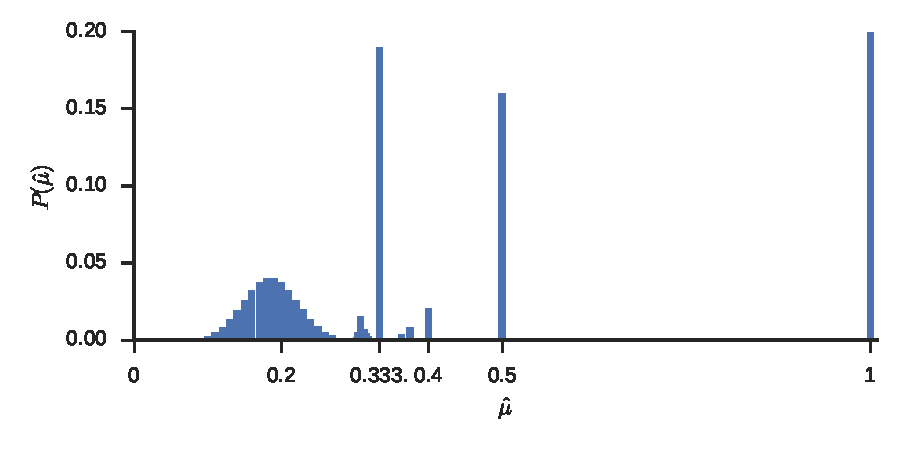
\includegraphics[scale=1]{extreme_early_stopping}
\end{figure}

There are a few key hueristic principles that are used to guide the development of bandit algorithms. The first is \emph{optimism in the face of uncertainty}. Applied to stochastic bandits, the optimism in the face of uncertainty princple suggests computing a plausible upper-bound for the expected reward of each arm, and selecting the arm with the highest upper bound. The optimism principle encourages exploitation and exploration because a high upper bound on the expected reward for an action implies either the expected reward or the uncertainty about the reward for that action is high. Thus selecting it yields either a good reward or useful information. 

\citet{Lai1985} leveraged the optimism in the face of uncertainty principle to develop an algorithm for specific families of reward distributions, including the expontial family. They showed that, for a given bandit problem, the pseudo-regret increased with $\bigo{log(T)}$ asymptopically and proved this is asymptopically efficient. However, their algorithm is complex and memory intensive to compute as, at each timestep, it relies on the entire sequence of rewards for each arm. \citet{Agrawal1995} developed a simpler algorithm that computed upper bounds based only on the mean of previous samples for each arm, whist retaining the logarithmic dependence on $T$. Finally, \citet{Auer2002} developed the UCB-1 algorithm, see algorithm \ref{alg:ucb-1}, which requires only that the reward distributions are bounded, and proved finite-time regret bounds. We now assume the rewards are bounded in $[0,1]$. The algorithm and regret bounds can be generalised to subgaussian reward distributions, see \citet{Bubeck2012}.

\begin{algorithm}[H]
\caption{UCB-1}\label{alg:ucb-1}
\begin{algorithmic}[1]
\STATE {\bf Input:} horizon $T$.
\STATE Play each arm once. 
\FOR{$t \in 1,\ldots,T$}
\STATE Count the number of times each arm has been selected previously $n_{t,i} = \sum_{s=1}^{t-1} \ind{a_s = i}$
\STATE Calculate the mean reward for each arm $\hat{\mu}_{t,i} = \frac{1}{n_{t,i}} \sum_{s=1}^{t-1}\ind{a_s = i}Y_t$
\STATE Select arm $a_t \in \argmax_{i = \set{1,...,k}}\left(\hat{\mu}_{t,i}+\sqrt{\frac{2 \log{t}}{n_{t,i}}}\right)$
\ENDFOR
\end{algorithmic}
\end{algorithm}
 
Let $\Delta_i = \mu_i - \mu^*$ be degree to which each arm is sub-optimal. The problem dependent psuedo-regret for UCB-1 is bounded by equation \ref{eqn:ucb_problem_dependent_regret} \citep{Bubeck2012},

\eqn {
\label{eqn:ucb_problem_dependent_regret}
\regret \leq & \sum_{i:\Delta_i > 0}\left(\frac{8\log(T)}{\Delta_i}+2 \right)
}

Somewhat unintuitively, the regret increases as the value of the arms gets closer together. This is because it becomes harder for the algorithm to identify the optimal arm. As the differences $\Delta_i \rightarrow 0$, the regret bound in \ref{eqn:ucb_problem_dependent_regret} blows up, however the regret itself does not - since although we may not be able to distinguish arms with very small $\Delta_i$ from the optimal arm, we also do not lose much by selecting them. The worst case occurs if all arms have the same expected reward $\mu$ except for the optimal arm which has reward $\mu^*=\mu+\Delta$, where $\Delta$ is just too small for the algorithm to learn to identify which arm is optimal given the horizon $T$. The regret cannot exceed what would be obtained by selecting the a sub-optimal arm in every timestep, $T\Delta$, so the worst case regret is bounded by the minimum of equation \ref{eqn:ucb_problem_dependent_regret} and $T\Delta$ which ia maximised when they are equal, see figure \ref{fig:ucb_regret_vs_delta}. By solving this equality for $\Delta$ one can show the worst case regret is bounded by equation \ref{eqn:ucb_worst_case_regret}, see \citet{Bubeck2012}.

\eqn{
\label{eqn:ucb_worst_case_regret}
\regret \in \bigo{\sqrt{kT\log(T)}}
}  

\begin{figure}
\caption{The regret bound in equation \ref{eqn:ucb_problem_dependent_regret} grows as the differences between the expected rewards for each arm shrink. The solid curve shows the mean (cummulative) regret, over a 1000 simulations for a 2-armed, bernoulli bandit with fixed horizon, $T = 500$, as a function of the difference in the expected reward for the arms $\Delta$. The dashed curves show the corresponding upper bounds; $T\Delta$ and equation \ref{eqn:ucb_problem_dependent_regret}}
\label{fig:ucb_regret_vs_delta}
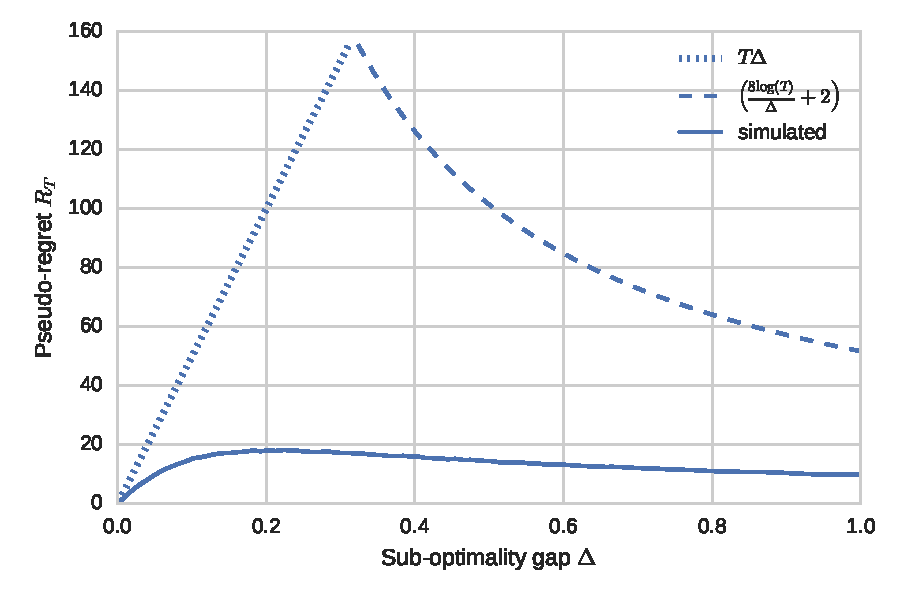
\includegraphics[scale=1]{ucb_regret_vs_delta}
\end{figure}

The form of the dependence on the number of arms $k$ and horizon $T$ differs between the problem dependent and worst case regret. The problem dependent regret grows linearly with the number of arms, $k$, and logarithmically with $T$. The difference stems from the fact the problem dependent regret defines how the regret grows for a given set of reward distributions as $T$ increases, whereas in the worst case regret, the gap between expected rewards is varied as a function of $T$. \citet{Auer1995} show that the worst case regret for the k-armed bandit problem is lower bounded by,

\eqn{
\label{eqn:k-arm-bandit-lower-bound}
\regret \in \bigomega{\sqrt{kT}}
}

Subtle modifications to the UCB algorithm can eliminate the logarithmic term equation \ref{eqn:ucb_worst_case_regret}. This yeilds regret $ \bigo{\sqrt{TK}}$ and closes the gap with the worst case lower bound \cite{Audibert2009,Lattimore2015}, whilst retaining a good problem dependent bound of the form achieved by UCB \cite{Lattimore2015}.

\begin{figure}
\caption{The actual performance of the UCB algorithm can be substantially better than suggested by the upper bound, particularly for small $T$. The solid curve shows the mean expected regret associated with the sequence of arms chosen by UCB-1 with $k=2$ arms and the rewards sampled from $bernoulli([.3,.7])$ over 1000 simulations. The dashed curve shows the corresponding upper bound given by the minimum of $T\Delta_{max}$ and equation\ref{eqn:ucb_problem_dependent_regret}.}
\label{fig:ucb_upperbound_vs_actual_performance}
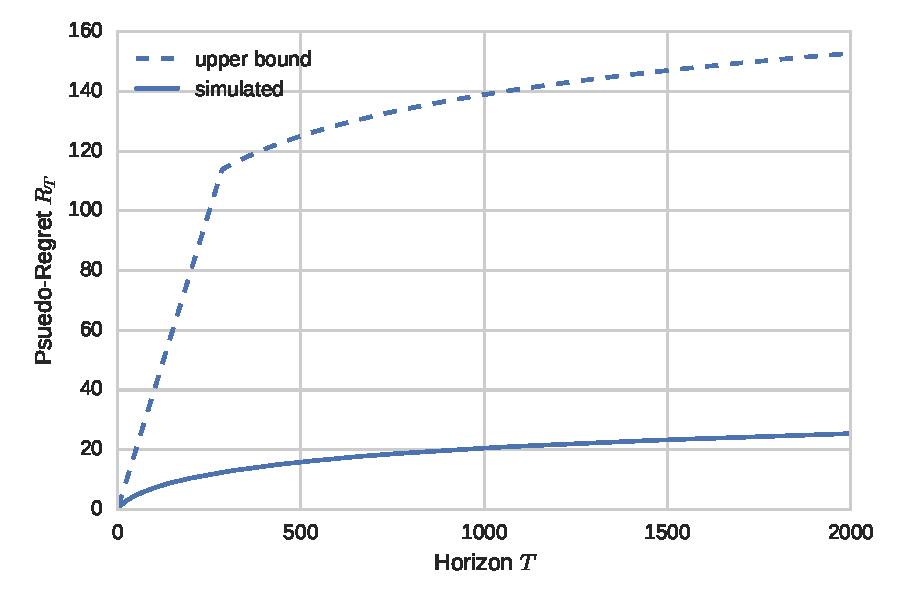
\includegraphics[scale=1]{upper_bound_vs_actual_average_regret}
\end{figure}

\subsection{Pure-exploration problems}
Another problem that has attracted a lot of recent attention \cite{Bubeck2009,Audibert2010,Gabillon2012,Karnin2013} within the stochastic multi-armed bandit framework is \textit{pure exploration} or \textit{best arm identification}. In this setting, the horizon $T$ represents a fixed budget for exploration after which the algorithm outputs a single best arm $i$. The performance of the algorithm is measured by the simple regret; the expected difference between the mean reward of the (truly) optimal arm and the mean reward of the arm selected by the algorithm.

\vspace{0.5cm}
\begin{definition}[Simple Regret]
\eqn{
\label{eqn:simple_regret}
\simpleregret=\mu_{i^*} - \E{\mu_{\hat i^*}}.
}
\end{definition}

The best arm identification problem arises naturally in applications where there is a testing or evaluation phase, during which regret is not incurred, followed by a commercialisation or exploitation phase. For example, many strategies might be assessed via simulation prior to one being selected and deployed. The worst case simple regret for a k-armed bandit is lower bounded by equation \ref{eqn:worst_case_simple_regret_lower_bound} (\citep{Bubeck2009}).

\eqn{
\label{eqn:worst_case_simple_regret_lower_bound}
\simpleregret \in \bigo{\sqrt{K/T}}
}


\todo{discuss the key ways in which the simple regret problem differs from cummulative regret}

Pure-exploration does not mean simply playing the arm with the widest uncertainty bounds. The goal is to be sure the arm we believe is optimal is in fact optimal at the end of the exploration period. 

\subsection{Adversarial Bandits}

Adversarial bandits are an alternate, widely studied, setting that relaxes the assumption that rewards are generated stochastically. Instead, simultaneously with the learner selecting an action $a_t$, a potentially malicious adversary selects the reward vector $\boldsymbol{Y}_t$. As in the stochastic setting, the learner then receives reward only for the selected action. 

\vspace{0.5cm}
\begin{definition}[Adversarial k-armed bandit problem]
Let $\actionspace = \set{1,...k}$ be the set of available actions.  In each round $t \in 1,...,T$, 
\begin{enumerate}
\item the world (or adversary) generates, but does not reveal, a vector or rewards $\vec{Y_t}=[Y_{t,1},...,Y_{t,k}]$. 
\item the learner selects an action $a_{t} \in \set{1,...,k}$, based on the actions and rewards from previous time-steps and a (potentially stochastic) \emph{policy} $\pi$
\item the learner observes and recieves (only) the reward for the selected action $Y_{t,a_t}$ 
\end{enumerate} 
\end{definition}

Adversaries that generate rewards independently of the sequence of actions selected by the learner in previous time steps are referred to as \emph{oblivous}, as opposed to \emph{non-oblivous} adversaries, which can generate rewards as a function of the history of the game. In the case of oblivous adversaries, we can also define the adversarial bandit problem by assuming the adversary generates the entire sequence of reward vectors before the game commences. 

The pseudo-regret for adversarial bandits is defined, in the same way as for stochastic bandits, as the difference between the reward obtained by playing the single arm with the highest expected reward in every round and the expected reward obtained by the algorithm.


\eqn{
\label{eqn:pseudo_regret-adversarial}
\regret(\pi) &= \max_{i \in \set{1,...,k}}\E{\sum_{t=1}^T{Y_{t,i}}} - \E{\sum_{t=1}^T{Y_{t,a_t}}}
}

The policy (or algorithm) used by the learner is avaiable to the adversary before the game begins, and there are no limitations placed on the amount of computation the adversary can perform in selecting the reward sequences. This implies the adversary can ensure that any learner with a deterministic policy suffers regret $\bigo{T}$ by forecasting their entire sequence of actions. For example, if the learner will play $a_1 = 1$ in the first round, then the adversary sets the reward $\vec{Y_1} = [0,1,1,...1]$, forcasts what action the learner will play in round 2, given they recieved a reward of 0 in round 1, and again generates the reward vector such that the action the learner will select obtains no reward, and all other actions obtain the maximum reward. This implies adversarial bandit policies must be sufficiently random to avoid such exploitation \footnote{The UCB algorithm, defined by algorithm \ref{alg:ucb-1}, is deterministic if the order in which arms are played during the first $k$ rounds is fixed and the method for selecting which arm to play when multiple-arms have the same upper-confidence bound is not-random (for example, select the arm one with the lowest index $i$).}

The seminal algorithm for adversarial bandits is Exp-3 \citep{Auer2002}, which, like UCB, obtains worst case psuedo-regret of $\bigo{\sqrt{TK\log(T)}}$  \cite{Auer1995}. Optimal algorithms, with $\regret = \bigo{\sqrt{TK}}$, have also been demonstrated for the oblivious adversarial setting \cite{Audibert2009}. The focus, for adversarial bandits, is on analysing the worst case regret because the problem dependent regret is not well defined without additional assumptions. However there has been recent work on developing algorithms that are optimised for both the adversarial and stochastic settings, in that they are sufficiently cautious to avoid linear regret in the adversarial setting but can nontheless obtain good problem dependent regret in more favourable enviroments \citep{bubeck2012bothworlds,Auer2016}. 

Adversarial bandits appear to be more applicable to real world problems because they do not assume that the rewards associated with each arm are constant over time or independent of the previous actions of the learner. However, psuedo-regret, as defined in equation \ref{eqn:pseudo_regret-adversarial}, is not a good measure of an algorithms performance in such cases because it is defined with respect to playing the single arm with the best average return over the game. In settings were the rewards change over time, the pseudo-regret can be negative, see figure \ref{fig:non-stationary-bandit}, so upper bounds on the psuedo-regret do not reflect how sub-optimal the algorithm may be. Adversarial bandit algorithms may perform better in non-stationary settings than standard stochastic policies to the extend that they explore more (to avoid the adversary simulating their behaviour), however it is preferable to develop algorithms specifically for non-stationary settings (subject to assumptions about how rapidly or frequently rewards can change), see for example \citep{garivier2008upper,Garivier2011a,Besbes2014}. 

\begin{figure}
  \caption{The pseudo-regret can be negative if rewards are non-stationary. This example shows the results of 1000 simulations of running the UCB-1 algorithm on a 2-armed bernoulli bandit problem where the expected rewards change linearly over time, up to a horizon $T=10,000$. Figure (a) shows the expected rewards of each arm, and the proportion of time that arm-1 is played, as a function of time. The single best-arm is arm-1 as it has the highest expected reward (averaged over $t$). An oracle that selects arm-1 in every round obtains an expected reward of $5,000$. However, despite not being designed to do so, the UCB-algorithm can adapt to the changing reward distribution to obtain costistently higher rewards. The distribution of regret over the 1000 simulations is shown in figure (b).}\label{fig:non-stationary-bandit}
    \begin{subfigure}[t]{0.49\textwidth}
	\centering   
	 \caption{Behaviour over time}\label{fig:non-stationary-bandit-time} 
         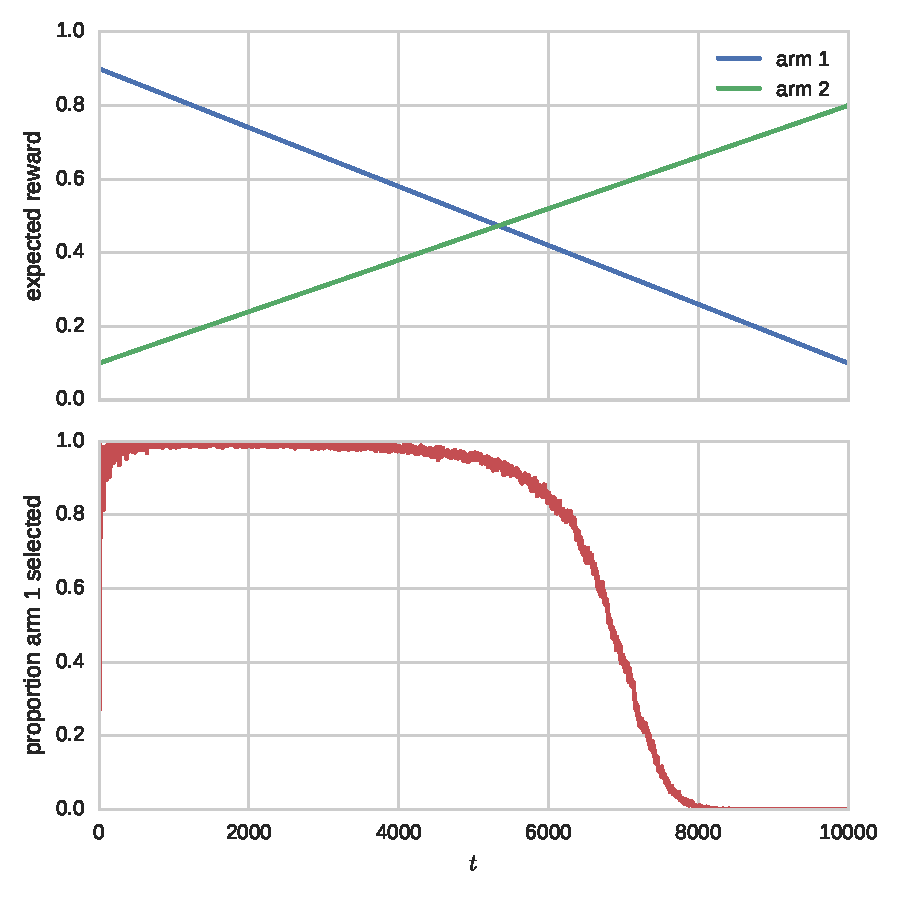
\includegraphics[scale=.5]{non-stationary-bandit-time}
\end{subfigure}
    \begin{subfigure}[t]{0.49\textwidth}
    \centering
     \caption{Cummulative regret distribution}
        \label{fig:non-stationary-bandit-regret}
        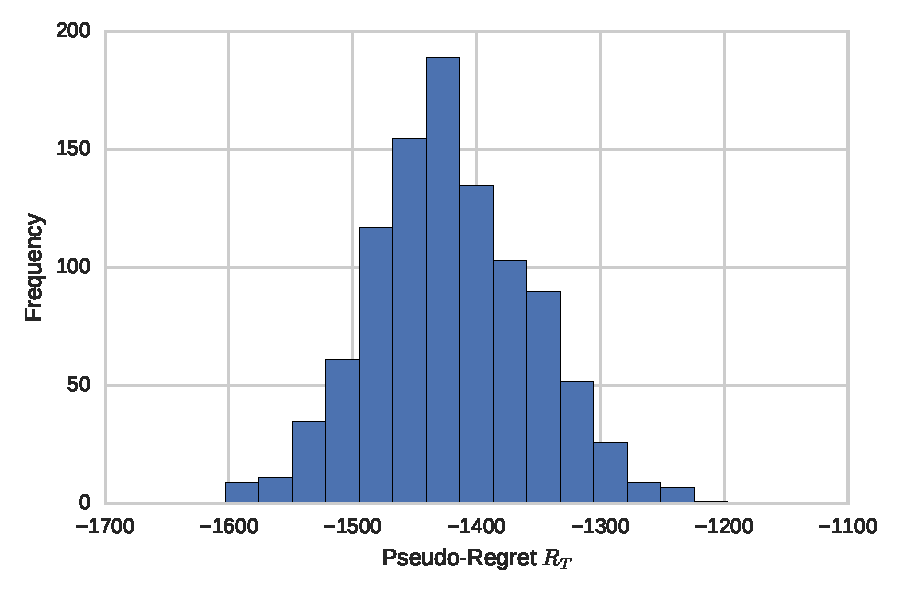
\includegraphics[scale=.5]{non-stationary-bandit-regret}
    \end{subfigure}
\end{figure}

\subsection{Contextual bandits}
Contextual bandits are a generalisation of multi-armed bandits. 

\vspace{0.5cm}
\begin{definition}[Contextual bandit problem]
Let $\P{\vec{Y},\vec{X}}$ be the joint distribution over the rewards for each action and some context $\vec{x} \sim \mathcal{X}$. In each round $t \in \set{1,...T}$, 
\begin{enumerate}
\item the world stochastically generates the vector of rewards for each action and the context, $([Y_{t,1},...,Y_{t,k}],\vec{x}_t) \sim \P{\vec{Y},\vec{X}}$ and reveals $\vec{x}_t$ to the learner
\item the learner selects an action $a_{t} \in \set{1,...,k}$, based on the context as well as actions and rewards from previous time-steps.
\item the learner observes and recieves (only) the reward for the selected action $Y_{t,a_t}$ 
\end{enumerate}
\end{definition} 

What are the reductions of contextual bandits to other problem (ie k armed-bandits?)

In the previous sections each decision was identical. If we were imaging treating patients, we assume that we have no additional information about each patient that is relevant to deciding how to treat them. However, in many key applications such as serving ads, etc, etc. we clearly do have additional information that we wish to take into account. In the contextual bandit setting the goal is to learn 

\eq {
\P{Y|a,x}
} 

As opposed to the standard bandit setting where we are attempting to estimate 

\eq{
\P{Y|a}
}

The formal definition of a contextual bandit problem is

The simplest way to generalise the standard bandit algorithms to the contextual case (where the context is discrete) is to simply have a separate standard bandit instance for each possible setting of the context. Regrettably this approach scales terribly with increasing complexity of the context. \todo{quantify this}. It cannot be applied at all if the context is continuous. 

The approach to solving this problem parallels those from supervised learning and continuous armed bandits. We make assumptions about the smoothness of the problem. Values of context that are similar should lead to comparable rewards for a given action. 

Regret bounds \todo {insert regret bounds for contextual bandits} 

It should be noted that there is an important difference between the approaches we can apply to the contextual bandit versus the supervised learning setting. As for the casual effect estimation problem, we cannot utilise cross-validation offline to select model parameters. This makes contextual bandit algorithms degrade faster than supervised learning ones as we add irrelevant variables. \todo{ask Tor if he thinks this is correct}

RUN A SIMULATION COMPARING HOW supervised learning and contextual bandits degrade as we add more features. What would be a fair comparison?

\subsubsection{Learning from logged bandit data}

\subsection{Markov decision processes}



A key limitation of the bandit setting is that 

This is reasonable in settings where we have many similar but independent units or individuals and the goal is to identify which action is optimal (in a given context), as occurs in standard experimental settings as well. 

Relation to SUTVA assumption, selecing a action for one 'unit' does not effect the reward distributions for other units. 

The reward of an action is not immediately known. - a long sequence of steps. Delayed reward. 



In the bandit setting the reward distributions for each arm are assumed to be fixed. A much studied generalisation is the Markov decision process or MDP. In an MDP we assume there the environment has some state. The reward an agent receives depends on the state of the environment and the action the agent selects. The environment then evolves stochastically depending on the agents action. Multi-armed bandits can be considered a single state MDP, where no matter what action the agent selects, the environment returns to that state. 

Insert a graphical representation of an MDP

What assumptions are required to make MDPs tractable. 

What is the basic algorithm (Q-learning)

What are the key results.

\subsubsection{Dynamic Systems}
\begin{itemize}
\item An explicit model of actions in a partially known system (eg HMM)
\item Feynman-Kac Lemma; Solving a PDE can be converted to a stochastic process
\end{itemize}







\subsection{The need to add structure}
The regret for a bandit problem grows linearly with the number of (sub-optimal) actions. This makes problems with large or infinite actions spaces intractable. REFERENCE equation showing linearity with arms. CHECK ITS TRUE. 

The classic multi-armed bandit is a powerful tool for sequential decision making. However, the regret grows linearly with the number of (sub-optimal) actions and many real world problems have large or even infinite action spaces. This has led to the development of a wide range of models that assume some structure across the reward distributions for different arms, for example generalised linear bandits \cite{filippi2010parametric}, dependent bandits \cite{Pandey2007}, X-armed bandits \cite{Bubeck2010} and Gaussian process bandits \cite{srinivas2009gaussian}, or that consider more complex feedback, for example the recent work on graph feedback \cite{Mannor2011,Lelarge2012,Alon2013,Buccapatnam2014,Kocak2014,Alon2015} and partial monitoring \cite{Piccolboni2001,Bartok2014}. 

\section{Questions}
\begin{enumerate}
\item When does the expected regret make sense as the thing we actually would wish to optimise? Is optimising the expected regret any different to optimising the psuedo-regret? Who is the definition of regret down to? Does this definition of regret come from learning with expert advise?
\item Is there a reference for the doubling trick? Is it an automatic way of converting a fixed horizon algorithm to an anytime one?
\item Why is the dependence on the number of arms $K$ in the problem dependent bounds but $\sqrt{K}$ in the worst case bounds?
\item rewards in the multi-armed bandit setting can be sampled from some joint distribution?
\item Is Learning from logged feedback data just covariate shift too?
\item In contextual bandits, does it ever make sense that $Y$ causes $X$? If the reward is some function of the action taken and the context, then the full vector of counterfactual outcomes $Y$ is never instantiated. Are there any implications of this for inference?
\item Why does anything solving a regression problem work in the anti-causal direction - it would seem to break the fundamental underlying assumption of additive noise?
\item is there a benchmark library of implementations of key bandit algorithms?
\item Bubeck 2012 states that if the adversary is oblivious, the psuedo-regret coincides with the standard regret, 'which is always the ultimate quantity of interest'. Why, they are not the same for stochastic bandits are they?
\item what is the worst-case regret of UCB in an adversarial setting?
\item is there a concept of problem dependent regret for adversarial bandits? Has there been analysis of the problem dependent regret for key adversarial algorithms such as EXP-3?
\item adversarial regret bounds for Thompson sampling, UCB with random arm selection from upper-bound set?
\item do continuous armed bandits implie that there are arms with any arbitrary gap in reward (including worst case gap for that T) and thus you always end up with something like worst case regret?)
\item in what real world setting do adversarial bandits potentially make sense?
\end{enumerate}


\chapter{Causal Bandits: Unifying the approaches}

\section{The framework}
\label{sec:intro_causal_bandit}
A natural way to connect the causal framework with the bandit setting is to model the action space as interventions on variables in a causal directed acyclic graph. Each possible assignment of variables to values is a potential action (or bandit arm), see figure \ref{fig:unify_frameworks} for a simple example. In some settings, it makes sense to restrict the action space available to the agent to a subset of all the possible actions, for example the set of single variable interventions. The reward could be a general function of the action selected and the final state of the graph. However for simplicity, we will consider the reward to be the value of a single specified node. We refer to these problems as \emph{causal bandit problems}. In this thesis I focus on the case where the causal graph is known. Extending this work to simultaneously learning the casual graph is discussed in \S\ref{sec:causal_bandit_discussion}.

\begin{figure}
\caption{A simple causal graphical model and corresponding complete action space. $W$ and $Z$ represent binary variables that can be intervened on and $Y$ represents the reward.}
\label{fig:unify_frameworks}
\centering
\begin{subfigure}[c]{0.3\textwidth}
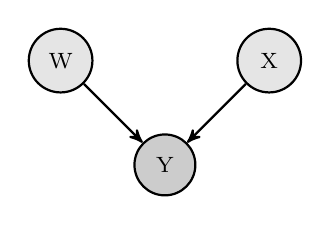
\begin{tikzpicture}[->,shorten >=0pt,shorten <=0pt,node distance=3em,thick,main node/.style={observed}, tg/.style={target}]
\node[main node](1){W};
\node[tg, below right=of 1](2){Y};
\node[main node, above right=of 2](3){X};
\path[]
	(1) edge (2)
	(3) edge (2);
\end{tikzpicture}
\end{subfigure}
\begin{subfigure}[t]{0.4\textwidth}
$\actionspace$ = \begin{tabular}{|c|}
	\hline
  $do(W=0,Z=0)$ \\
  $do(W=0,Z=1)$ \\
  $do(W=1,Z=0)$ \\
  $do(W=1,Z=1)$ \\
  \hline
  $do(W=0)$ \\
  $do(W=1)$ \\
  $do(Z=0)$ \\
  $do(Z=1)$ \\
  $do()$ \\
  \hline
\end{tabular}
\end{subfigure}
\end{figure} 

The type of problem we are concerned with is best illustrated with an example. Consider a farmer wishing to optimise the yield of her crop. She knows that crop yield is only affected by temperature, a particular soil nutrient, and moisture level but the precise effect of their combination is unknown. In each season the farmer has enough time and money to intervene and control at most one of these
variables: deploying shade or heat lamps will set the temperature to be low or high; the nutrient can be added or removed through a choice of fertilizer; and irrigation or rain-proof covers will keep the soil wet or dry. When not intervened upon, the temperature, soil, and moisture vary naturally from season to season due to weather conditions and these are all observed along with the final crop yield at the end of each season. How might the farmer best experiment to identify the single, highest yielding intervention in a limited number of seasons?

We will assume each variable only takes on a finite number of distinct values. (The path to relaxing this assumption would be through levering the work on continuous armed bandits). The \emph{parents} of a variable $X_i$, denoted $\parents{X_i}$, is the set of all variables $X_j$ such that there is an edge from $X_j$ to $X_i$ in $\mathcal{G}$. An \emph{intervention or action (of size $n$)}, denoted $do(\vec{X}=\vec{x})$, assigns the values $\vec{x}=\{x_1, \ldots, x_n\}$ to the corresponding variables $\vec{X}=\{X_1, \ldots, X_n\} \subset \mathcal{X}$ with the empty intervention (where no variable is set) denoted $do()$. We denote the expected reward for the action $a = do(\vec{X} = \vec{x})$ by $\mu_{a} := \E{Y | do(\vec{X} = \vec{x})}$ and 
the optimal expected reward by $\mu^* := \max_{a\in\actions} \mu_{a}$. 

\vspace*{.5cm}
\begin{definition}[Causal bandit problem]
A learner for a casual bandit problem is given the casual model’s graph $G$ over variables $\mathcal{X}$ and a set of allowed actions $\actionspace$. Each action $a \in \actionspace$ assings a value to a subset of the variables in $\mathcal{X}$. One variable $Y \in \mathcal{X}$ is designated as the \emph{reward variable} and takes on values in $\{0, 1\}$.

The causal bandit game proceeds over $T$ rounds. In each round $t$, the learner:
\begin{enumerate}
\item \emph{observes} the value of a subset of the variables $\vec{X}^c_t$,
\item \emph{intervenes} by choosing $a_t = do(\vec{X}_t = \vec{x}_t) \in \mathcal{A}$ based on previous observations, and finally
\item \emph{observes} sampled values for another subset of variables $\vec{X}^o_t$ drawn from $\P{\vec{X}^o_t | do(\vec{X}_t = \vec{x}_t)}$ including the \emph{reward} $Y_t \in \{0,1\}$.
\end{enumerate} 

We refer to the set of variables that can be observed prior to selecting an action $\vec{X}^c$ as contextual variables and the set of variables observed after the action is chosen, $\vec{X}^o$, as post-action feedback variables. Note that $\vec{X}^c$ and $\vec{X}^o$ need not be disjoint. A variable may be observed both prior to and after the agent selects an action, and the action may change its value. The objective of the learner is to minimise either the simple (equation \ref{}) or cummulative regret (equation \ref{}). 

\end{definition}

The causal bandit problem takes on characteristics of different bandit settings depending on the actionspace $\actionspace$, which variables are observable prior to selecting an action and on which variables we recieve post-action feedback. If feedback is recieved only on the reward node $\vec{X}^o = \set{Y}$, as in the standard bandit setting, then the do-calculus can be applied to eliminate some actions immediately, before any experiments are performed and then a standard bandit algorithm can be run on the remaining actions, see figure \ref{fig:cholesterol_graph} as an example. If we recieve post-action feedback on additional nodes the problem can be more interesting. In addition to being able to eliminate some actions prior to sampling any data as in the previous case, taking one action may give us some information on actions that were not selected. Consider again the model in figure \ref{fig:unify_frameworks}. The causal structure implies: 

\eq{
P(Y|do(W = 0)) &= P(Y|do(),W = 0) \\
&= P(Y|do(X=0),W=0)P(X=0)+P(Y|do(X=1),W=0)P(X=1) 
}

\begin{figure}
\caption{Example causal graph (based on \cite{Koller2009}) where the outcome of interest (reward) is cholesterol level . The do-calculus can be applied to eliminate some actions immediately without the need to do any experiments. For example, no actions involving 'Test Result' need to be considered and interventions on 'Diet' do not need to be considered in conjunction with any other variables.}
\label{fig:cholesterol_graph}
\centering
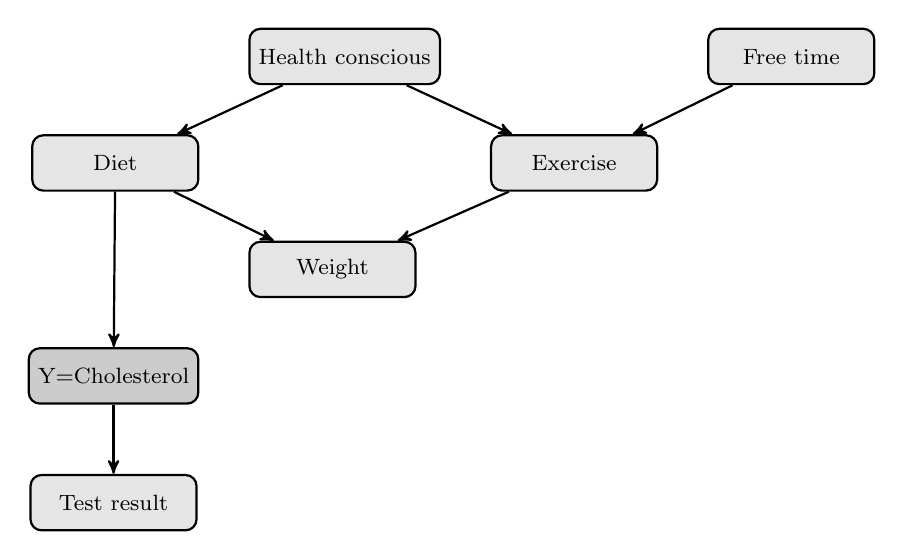
\begin{tikzpicture}[->,shorten >=0pt,shorten <=0pt,node distance=2.5em,thick,node/.style={observedrect},tg/.style={targetrect}]
\node[node](1){Health conscious};
\node[node, below left=of 1](2){Diet};
\node[node, below right=of 1](3){Exercise};
\node[node, below right=of 2](4){Weight};
\node[tg,below left=of 4](5){Y=Cholesterol};
\node[node, below =of 5](6){Test result};
\node[node, above right=of 3](7){Free time};
\path[]
	(1) edge (2) edge (3)
	(2) edge (4) edge (5)
	(3) edge (4)
	(5) edge (6)
	(7) edge (3);
\end{tikzpicture}
\end{figure}


Thus we gain information about the reward for the action $do(W=0)$ from selecting the action $do()$ or $do(X = x)$ and then observing $W = 0$.  We only get this form of side information for actions that don't specify the value of every variable, for example those in the bottom half of the table in figure \ref{fig:unify_frameworks}. If additional variables are only observed before an intervention is selected the causal bandit problem reduces to stochastic contextual bandits, which are already reasonably well understood \citep{Agarwal2014}.

We note that classical $K$-armed stochastic bandit problem can be recovered in our framework by considering a simple causal model with one edge connecting a single variable $X$ that can take on $K$ values to a reward variable $Y \in \set{0,1}$ where $\P{Y = 1|X} = r(X)$ for some arbitrary but unknown, real-valued function $r$. The set of allowed actions in this case is $\mathcal{A} = \{ do(X = k) \colon k \in \{1, \ldots, K\}\}$. Conversely, any causal bandit problem can be reduced to a classical stochastic $|\mathcal{A}|$-armed bandit problem by treating each possible intervention as an independent arm and ignoring all sampled values for the observed variables except for the reward. However, the number of actions or arms grows exponentially with the number of variables in the graph making it important to develop algorithms that leverage the graph structure and additional observations.

\section{Causal bandits with post action feedback}

We now focus on causal bandit problems with post-action feedback, in which the value of all the variables are observed after an intervention is selected, and where the goal of the learner is to minimise the simple regret. I presented this work at NIPS 2016 \citep{NIPS2016_6195}.

\paragraph{Related Work} As alluded to above, causal bandit problems can be treated as classical multi-armed bandit problems by simply ignoring the causal model and extra observations and applying an existing best-arm identification algorithm with well understood simple regret guarantees \citep{Jamieson2013}. However, as we show in \S\ref{sec:simple-regret}, ignoring the extra information available in the non-intervened variables yields sub-optimal performance.

A well-studied class of bandit problems with side information are ``contextual bandits''~\cite{Langford2008,Agarwal2014}. Our framework bears a superficial similarity to contextual bandit problems since the extra observations on non-intervened variables might be viewed as context for selecting an intervention. 
However, a crucial difference is that in our model the extra observations are only revealed \emph{after} selecting an intervention and hence cannot be used as context. 

There have been several proposals for bandit problems where extra feedback is received after an action is taken.
Most recently, \citet{Alon2015}, \citet{Kocak2014} have considered very general models related to partial monitoring games~\citep{Bartok2014} where rewards on unplayed actions are revealed according to a feedback graph. As we discuss in \S\ref{sec:causal_bandit_discussion}, the parallel bandit problem can be captured in this framework, however the regret bounds are not optimal in our setting. They also focus on cumulative regret, which cannot be used to guarantee low simple regret~\citep{Bubeck2009a}. The partial monitoring approach taken by \cite{wu2015online} could be applied (up to modifications for the simple regret) to the parallel bandit, but the resulting strategy would need to know the likelihood of each factor in advance, while our strategy learns this online. \citet{Yu2009} utilize extra observations to detect changes in the reward distribution, whereas we assume fixed reward distributions and use extra observations to improve arm selection. \citet{Avner2012} analyse bandit problems where the choice of arm to pull and arm to receive feedback on are decoupled. The main difference from our present work is our focus on simple regret and the more complex information linking rewards for different arms via causal graphs. To the best of our knowledge, our paper is the first to analyse simple regret in bandit problems with extra post-action feedback.


%\citet{Yu2009} consider bandit problems where a learner chooses an arm to play as well as set of arms to observe rewards for in a stochastic setting where the reward distributions can change infrequently and the aim is to minimize cumulative regret. They use extra observations to detect changes whereas we assume fixed reward distributions and use extra observations to improve arm selection.
% Partial monitoring is a very general framework for for decoupling the feedback from the action and reward. It can be used to classify problems into one of four categories, trivial with no regret, easy with $R_T = \bigthetatilde{\sqrt{T}}$ , hard with $R_T = \bigtheta{T^{2/3}}$ and hopeless with $R_T = \bigomega{T}$ \cite{Bartok2014}. Partial monitoring algorithms yield results that are optimal with respect the horizon $T$ but not other parameters, such as $K$, which is the key focus of incorporating causal structure. 

Two pieces of recent work also consider applying ideas from causal inference to bandit problems.
\citet{Bareinboim2015} demonstrate that in the presence of confounding variables the value that a variable would have taken had it not been 
intervened on can provide important contextual information. Their work differs in many ways. For example, the focus is on the cumulative regret and
the context is observed before the action is taken and cannot be controlled by the learning agent.  

%\todof{write one sentence to explain how their work is different to ours}

 \citet{Ortega2014thompson} present an analysis and extension of Thompson sampling assuming actions are causal interventions. Their focus is on causal induction (\ie, learning an unknown causal model) instead of exploiting a known causal model. Combining their handling of  causal induction with our analysis is left as future work.
% Key to Elias' paper is: observing the action an agent would take if it were allowed to make its natural choice can provide some information about hidden confounders that influence both the reward and the choice of action. Therefore, incorporating an agents natural choice as context may outperform a standard bandit that does not use that context. (Note: even in the presence of hidden confounders, including the agents natural choice as context only may improve the results. It is easy to come up with a counter example in which it does not).

The truncated importance weighted estimators used in \S\ref{sec:simple-regret-general} have been studied before in a causal framework by \citet{Bottou2013a}, 
where the focus is on learning from observational data, but not controlling the sampling process. They also briefly discuss some of the issues 
encountered in sequential design, but do not give an algorithm or theoretical results for this case.


\subsection{The parallel bandit problem}
\label{sec:simple-regret}
In this section we propose and analyse an algorithm for achieving the optimal regret in a natural special case of the causal bandit problem which we call the {\it parallel bandit}.
It is simple enough to admit a thorough analysis but rich enough to model the type of problem discussed in \S\ref{sec:intro_causal_bandit}, including the farming example. It also suffices to witness the regret gap between algorithms that make use of causal models and those which do not.

The causal model for this class of problems has $N$ binary variables $\{ X_1, \ldots, X_N \}$ where each $X_i \in \{0,1\}$ are independent causes of a reward variable $Y \in \set{0,1}$, as shown in Figure~\ref{fig:parallel}. All variables are observable and the set of allowable actions are all size 0 and size 1 interventions: $\mathcal{A} = \set{do()} \cup \set{ do(X_i = j) \colon 1 \leq i \leq N \text{ and } j \in \set{0,1}}$

In the farming example from the introduction, $X_1$ might represent temperature (\eg, $X_1=0$ for low and $X_1=1$ for high). The interventions $do(X_1 = 0)$ and $do(X_1 = 1)$ indicate the use of shades or heat lamps to keep the temperature low or high, respectively.

\begin{figure}
  \caption{Causal Models}\label{fig:causalmodels}
    \begin{subfigure}[t]{0.34\textwidth}
	\centering   
	 \caption{Parallel graph}\label{fig:parallel} 
          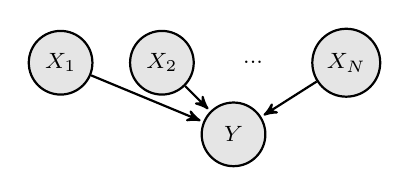
\begin{tikzpicture}[->,>=stealth',shorten >=1pt,auto,node distance=.45cm,
  thick,main node/.style={observed}, hidden/.style={empty},background rectangle/.style={fill=olive!45}]
%every node/.style={scale=0.6}
 %nodes
\node[main node](1){$X_{1}$};
\node[main node, right=of 1](2){$X_{2}$};
\node[hidden, right=of 2](3){$...$};
\node[main node, right=of 3](4){$X_{N}$};
\node[main node, below right=of 2](5){$Y$};
 \path[every node/.style={font=\tiny}]
    (1) edge (5)
    	(2) edge (5)
    (4) edge (5);
\end{tikzpicture} 
\end{subfigure}
    \begin{subfigure}[t]{0.25\textwidth}
    \centering
     \caption{Confounded graph}
        \label{fig:causalStructure_confounded}
        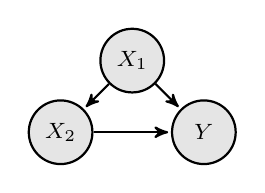
\begin{tikzpicture}[->,>=stealth',shorten >=1pt,auto,node distance=.45cm,
  thick,main node/.style={observed}, hidden/.style={empty},background rectangle/.style={fill=olive!45}]
\node[main node](1){$X_1$};
\node[main node, below left=of 1](2){$X_2$};
\node[main node, below right=of 1](4){$Y$};
 \path[every node/.style={font=\tiny}]
    (1) edge (2)
    (1) edge (4)
    (2) edge (4);
\end{tikzpicture}
    \end{subfigure}
    \begin{subfigure}[t]{0.4\textwidth}
    \centering
     \caption{Chain graph}
        \label{fig:causalchain}
         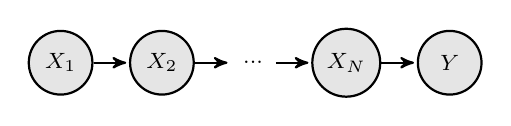
\begin{tikzpicture}[->,>=stealth',shorten >=1pt,auto,node distance=.45cm,
  thick,main node/.style={observed}, hidden/.style={empty},background rectangle/.style={fill=olive!45}]
\node[main node](1){$X_{1}$};
\node[main node, right=of 1](2){$X_{2}$};
\node[hidden, right=of 2](3){$...$};
\node[main node, right=of 3](4){$X_{N}$};
\node[main node, right=of 4](5){$Y$};
 \path[every node/.style={font=\tiny}]
    (1) edge (2)
  	(2) edge (3)
    (3) edge (4)
    (4) edge (5);
\end{tikzpicture}
    \end{subfigure}
\end{figure}


In each round the learner either purely observes by selecting $do()$ or sets the value of a single variable. The remaining variables are simultaneously set by independently biased coin flips. The value of all variables are then used to determine the distribution of rewards for that round. Formally, when not intervened upon we assume that each $X_i \sim \bernoulli(q_i)$ where $\vec{q} = (q_1, \ldots, q_N) \in [0,1]^N$ so that $q_i = \P{X_i = 1}$.

The value of the reward variable is distributed as $\P{Y = 1|\vec{X}} = r(\vec{X})$ where 
$r : \{0,1\}^N \to [0,1]$ is an arbitrary, fixed, and unknown function. 
In the farming example, this choice of $Y$ models the success or failure of a seasons crop, 
which depends stochastically on the various environment variables.


\paragraph{The Parallel Bandit Algorithm}
%\label{sub:par-bandit-alg}
The algorithm operates as follows. For the first $T/2$ rounds it chooses $do()$ to collect observational data. As the only link from each $X_1,\ldots,X_N$ to $Y$ is a direct, causal one, $\P{Y|do(X_i=j)}=\P{Y|X_i=j}$. Thus we can create good estimators for the returns of the actions $do(X_i = j)$ for which $\P{X_i = j}$ is large. The actions for which $\P{X_i = j}$ is small may not be observed (often) so  estimates of their returns could be poor. To address this, the remaining $T/2$ rounds are evenly split to estimate the rewards for these infrequently observed actions. The difficulty of the problem depends on $\vec{q}$ and, in particular, how many of the variables are unbalanced (\ie, small $q_i$ or $(1-q_i)$). For $\tau \in [2...N]$ let $I_\tau = \set{ i : \min\set{q_i, 1-q_i} < \frac{1}{\tau}}$. Define

\eq{
\label{eq:m-simple}
m(\vec{q}) = \min \set{ \tau : |I_{\tau}| \leq \tau}\,.
}


\begin{algorithm}[H]
\caption{Parallel Bandit Algorithm}\label{alg:simple}
\begin{algorithmic}[1]
\STATE {\bf Input:} Total rounds $T$ and $N$.
\FOR{$t \in 1,\ldots,T / 2$}
\STATE Perform empty intervention $do()$
\STATE Observe $\vec{X}_t$ and $Y_t$
\ENDFOR
\FOR{$a = do(X_i = x) \in \actions$}
\STATE Count times $X_i = x$ seen: $T_a = \sum_{t=1}^{T/2} \ind{X_{t,i} = x}$
\STATE Estimate reward: $\hat{\mu}_a = \frac{1}{T_a} \sum_{t=1}^{T/2} \ind{X_{t,i} = x} Y_t$ \\[0.2cm]
\STATE Estimate probabilities: $\hat{p}_a = \frac{2 T_a}{T}$,\,\, $\hat q_i = \hat p_{do(X_i = 1)}$
\ENDFOR
\STATE Compute $\hat{m} = m(\vec{\hat q})$ and $A = \set{a \in \actions \colon \hat{p}_a \leq \frac{1}{\hat m}}$.
\STATE Let $T_A := \frac{T}{2 |A|}$ be times to sample each $a\in A$.
\FOR{$a = do(X_i = x) \in A$}
\FOR{$t \in 1,\ldots,T_A$}
\STATE Intervene with $a$ and observe $Y_t$
\ENDFOR
\STATE Re-estimate $\hat{\mu}_a = \frac{1}{T_A} \sum_{t=1}^{T_A} Y_t$
\ENDFOR
\RETURN estimated optimal $\hat{a}^*_T \in \argmax_{a\in\actions} \hat{\mu}_a$
\end{algorithmic}
\end{algorithm}

$I_\tau$ is the set of variables considered unbalanced and we tune $\tau$ to trade off identifying the low probability actions against not having too many of them, so as to minimise the worst-case simple regret. When $\vec{q} = (\frac{1}{2}, \ldots, \frac{1}{2})$ we have $m(\vec{q}) = 2$ and when $\vec{q} = (0, \ldots, 0)$ we have $m(\vec{q}) = N$. We do not assume that $\vec{q}$ is known, thus Algorithm \ref{alg:simple} also utilises the samples captured during the observational phase to estimate $m(\vec{q})$. Although very simple, the following two theorems show that this algorithm is effectively optimal.


\begin{theorem}\label{thm:uq-simple}
Algorithm \ref{alg:simple} satisfies
\eq{
\simpleregret \in \bigo{\sqrt{\frac{m(\vec{q})}{T}\log\left(\frac{NT}{m(\vec{q})}\right)}}\,.
}
\end{theorem}


\begin{theorem}\label{thm:lower}
For all strategies and $T$, $\vec{q}$, there exist rewards such that
$\displaystyle \simpleregret 
\in \Omega\left(\sqrt{\frac{m(\vec{q})}{T}}\right)$.
\end{theorem}

The proofs of Theorems \ref{thm:uq-simple} and \ref{thm:lower} follow by carefully analysing the concentration
of $\hat p_a$ and $\hat m$ about their true values and may be found in Sections \ref{sec:thm:uq-simple} and \ref{sec:thm:lower} respectively.

%We prove a lower bound on the simple regret that matches up to logarithmic factors the upper bound given in Theorem \ref{thm:uq-simple}. 
By utilising knowledge of the causal structure, Algorithm \ref{alg:simple} effectively only has to explore the $m(\vec{q})$ 'difficult' actions. Standard multi-armed bandit algorithms must explore all $2N$ actions and thus achieve regret  $\smash{\Omega(\sqrt{N/T})}$. Since $m$ is typically much smaller than $N$, the new algorithm can significantly outperform classical bandit algorithms in this setting. In practice, you would combine the data from both phases to estimate rewards for the low probability actions. We do not do so here as it slightly complicates the proofs and does not improve the worst case regret.

\subsection{General graphs}
\label{sec:simple-regret-general}
We now consider the more general problem where the graph structure is known, but arbitrary. For general graphs, $\P{Y|X_i=j} \neq \P{Y|do(X_i=j)}$ (correlation is not causation). However, if all the variables are observable, any causal distribution $\P{X_1...X_N|do(X_i=j)}$ can be expressed in terms of observational distributions via the truncated factorisation formula \citep{Pearl2000}. 
\eq{
\P{X_1...X_N|do(X_i=j)} = 
\prod_{k \neq i}\P{X_k|\parents{X_k}}\delta(X_i - j)\,, 
} 
where $\parents{X_k}$ denotes the parents of $X_k$ and $\delta$ is the Dirac delta function. 

We could naively generalise our approach for parallel bandits by observing for $T/2$ rounds, applying the truncated product factorisation to 
write an expression for each $\P{Y|a}$ in terms of observational quantities and explicitly playing the actions for which the observational 
estimates were poor. However, it is no longer optimal to ignore the information we can learn about the reward for intervening on one variable 
from rounds in which we act on a different variable. Consider the graph in Figure \ref{fig:causalchain} and suppose each variable deterministically 
takes the value of its parent, $X_k = X_{k-1}$ for $k\in {2,\ldots,N}$ and $\P{X_1} = 0$. We can learn the reward for all the interventions $do(X_i = 1)$ 
simultaneously by selecting $do(X_1 = 1)$, but not from $do()$. In addition, variance of the observational estimator for $a = do(X_i = j)$ can be 
high even if $\P{X_i = j}$ is large. Given the causal graph in Figure \ref{fig:causalStructure_confounded}, $\P{Y|do(X_2= j)} = \sum_{X_1}\P{X_1}\P{Y|X_1, X_2 = j}$. 
Suppose $X_2 = X_1$ deterministically, no matter how large $\P{X_2 = 1}$ is we will never observe $(X_2=1,X_1 = 0)$ and so cannot 
get a good estimate for $\P{Y|do(X_2=1)}$. 

To solve the general problem we need an estimator for each action that incorporates information obtained from every other action and a way to optimally 
allocate samples to actions. To address this difficult problem, we assume the conditional interventional distributions $\P{\parents{Y}|a}$ (but not $\P{Y|a}$) 
are known. These could be estimated from experimental data on the same covariates but where the outcome of interest differed, such that $Y$ was not included, 
or similarly from observational data subject to identifiability constraints. Of course this is a somewhat limiting assumption, but seems like a natural place to
start. The challenge of estimating the conditional distributions for all variables in an optimal way is left as an interesting future direction.
Let $\eta$ be a distribution on available interventions $a \in \calA$ so $\eta_a \geq 0$ and $\sum_{a \in \calA} \eta_a = 1$. 
Define $Q = \sum_{a \in \calA} \eta_a \P{\parents{Y}|a}$ to be the mixture distribution over the interventions with respect to $\eta$.



\begin{algorithm}[H]
\caption{General Algorithm}\label{alg:general}
\begin{algorithmic}
\STATE {\bf Input:} $T$, $\eta \in [0,1]^{\calA}$, $B \in [0,\infty)^{\calA}$
\FOR{$t \in \set{1,\ldots,T}$}
\STATE Sample action $a_t$ from $\eta$
\STATE Do action $a_t$ and observe $X_t$ and $Y_t$
\ENDFOR
\FOR{$a \in \calA$}
\STATE
\eq {
\hat \mu_a =  \frac{1}{T} \sum_{t=1}^T Y_t R_a(X_t)  \ind{R_a(X_t) \leq B_a}
}
\ENDFOR
\STATE {\bf return} $\hat a^*_T = \argmax_a \hat \mu_a$
\end{algorithmic}
\end{algorithm}


Our algorithm samples $T$ actions from $\eta$ and uses them to estimate the returns $\mu_a$ for all $a \in \calA$ simultaneously via a truncated importance weighted estimator. Let $\parents{Y}(X)$ denote the realisation of the variables in $X$ that are parents of Y and define $R_a(X) = \frac{\Pn{a}{\parents{Y}(X)}}{\Q{\parents{Y}(X)}}$

\eq {
\hat \mu_a =  \frac{1}{T} \sum_{t=1}^T Y_t R_a(X_t)  \ind{R_a(X_t) \leq B_a}\,, 
} 

where $ B_a \geq 0$  is a constant that tunes the level of truncation to be chosen subsequently. The truncation introduces a bias in the estimator, but simultaneously chops the potentially heavy tail that is so detrimental to its concentration guarantees. 

The distribution over actions, $\eta$ plays the role of allocating samples to actions and is optimised to minimise the worst-case simple regret. Abusing notation we define $m(\eta)$ by
\eq{
m(\eta) = \max_{a \in \calA} \EEa\left[\frac{\Pn{a}{\parents{Y}(X)}}{\Q{\parents{Y}(X)}}\right]\,,\text{ where } \EEa \text{ is the expectation with respect to } \Pn{a}.
}

We will show shortly that $m(\eta)$ is a measure of the difficulty of the problem that approximately coincides with the version for parallel bandits, justifying the name overloading.

\begin{theorem}\label{thm:general}
If Algorithm \ref{alg:general} is run with $B \in \R^{\calA}$ given by $B_a = \sqrt{\frac{m(\eta)T}{\log\left(2T|\calA|\right)}}\,.$

\eq{
\simpleregret \in \bigo{\sqrt{\frac{m(\eta)}{T} \log\left(2T|\calA|\right)}}\,.
}
\end{theorem}

The proof is in Section \ref{sec:thm:general}.

Note the regret has the same form as that obtained for Algorithm \ref{alg:simple}, with $m(\eta)$ replacing $m(q)$. Algorithm \ref{alg:simple} assumes only the graph structure and not knowledge of the conditional distributions on $X$. Thus it has broader applicability to the parallel graph than the generic algorithm given here. We believe that Algorithm \ref{alg:general} with the optimal choice of $\eta$ is close to mini-max optimal, but leave lower bounds
for future work.


\paragraph{Choosing the Sampling Distribution} Algorithm \ref{alg:general} depends on a choice of sampling distribution $\operatorname{Q}$ that is determined by $\eta$. In light of Theorem \ref{thm:general}
a natural choice of $\eta$ is the minimiser of $m(\eta)$.
\eq{
\eta^* 
= \argmin_\eta m(\eta) = \argmin_\eta \underbrace{\max_{a \in \calA} \EEa \left[\frac{\Pn{a}{\parents{Y}(X)}}{\sum_{b \in \calA} \eta_b \Pn{b}{\parents{Y}(X)}}\right]}_{m(\eta)}\,.
}
Since the mixture of convex functions is convex and the maximum of a set of convex functions is convex, we see that $m(\eta)$ is convex (in $\eta$).
Therefore the minimisation problem may be tackled using standard techniques from convex optimisation. The quantity $m(\eta^*)$ may be interpreted as the minimum achievable worst-case variance of the importance weighted estimator. In the experimental section we present some special cases, but for now we give two simple results. The first shows that $|\calA|$ serves as an upper bound on $m(\eta^*)$.

\begin{proposition}\label{pro:m-bound}
$m(\eta^*) \leq |\calA|$. \textit{Proof.} 
\textup{By definition, $m(\eta^*) \leq m(\eta)$ for all $\eta$. Let $\eta_a = 1/|\calA|\,\forall a$.}
\eq{
m(\eta) 
= \max_a \EEa\left[\frac{\Pn{a}{\parents{Y}(X)}}{\Q{\parents{Y}(X)}}\right] 
\leq \max_a \EEa\left[\frac{\Pn{a}{\parents{Y}(X)}}{\eta_a \Pn{a}{\parents{Y}(X)}}\right] 
= \max_a \EEa\left[\frac{1}{\eta_a}\right] = |\calA| %\qedhere
}
\end{proposition} 

The second observation is that, in the parallel bandit setting, $m(\eta^*) \leq 2m(\boldsymbol{q})$. This is easy to see by letting $\eta_a = 1/2$ for $a = do()$ and $\eta_a = \ind{\P{X_i = j} \leq 1/m(\boldsymbol{q})} / 2m(\boldsymbol{q})$ for the actions corresponding to $do(X_i=j)$, and applying an argument like that for Proposition~\ref{pro:m-bound}. The proof is in section \ref{sec:m-equivelence}.

\begin{remark}\label{rem:truncate}
The choice of $B_a$ given in Theorem \ref{thm:general} is not the only possibility. As we shall see in the experiments, it is 
often possible to choose $B_a$ significantly
larger when there is no heavy tail and this can drastically improve performance by eliminating the bias. This is especially true when the ratio $R_a$ is never too large
and Bernstein's inequality could be used directly without the truncation. For another discussion see the article by \citet{Bottou2013a} who also use importance weighted estimators
to learn from observational data.
\end{remark}


\subsection{Experiments}
We compare Algorithms \ref{alg:simple} and \ref{alg:general} with the Successive Reject algorithm of \cite{audibert2010best}, Thompson Sampling and UCB under a variety of conditions. Thomson sampling and UCB are optimised to minimise cumulative regret. We apply them in the fixed horizon, best arm identification setting by running them up to horizon $T$ and then selecting the arm with the highest empirical mean. The importance weighted estimator used by Algorithm \ref{alg:general} is not truncated, which is justified in this setting by Remark \ref{rem:truncate}. 

Throughout we use a model in which $Y$ depends only on a single variable $X_1$ (this is unknown to the algorithms). $Y_t \sim \bernoulli(\frac{1}{2}+\epsilon)$ if $X_1=1$ and $Y_t \sim \bernoulli(\frac{1}{2}-\epsilon')$ otherwise, where $\epsilon' = q_1\epsilon/(1-q_1)$. This leads to an expected reward of $\frac{1}{2}+\epsilon$ for $do(X_1=1)$, $\frac{1}{2}-\epsilon'$ for $do(X_1=0)$ and $\frac{1}{2}$ for all other actions. We set $q_i = 0$ for $i \leq m$ and $\frac{1}{2}$ otherwise. Note that changing $m$ and thus $\boldsymbol{q}$ has no effect on the reward distribution. For each experiment, we show the average regret over 10,000 simulations with error bars displaying three standard errors. The code is available from \url{<https://github.com/finnhacks42/causal_bandits>} 

In Figure \ref{fig:simple_vs_m} we fix the number of variables $N$ and the horizon $T$ and compare the performance of the algorithms as $m$ increases. The regret for the Successive Reject algorithm is constant as it depends only on the reward distribution and has no knowledge of the causal structure. For the causal algorithms it increases approximately with $\sqrt{m}$. As $m$ approaches $N$, the gain the causal algorithms obtain from knowledge of the structure is outweighed by fact they do not leverage the observed rewards to focus sampling effort on actions with high pay-offs.


\begin{figure}[h]
    \begin{subfigure}[t]{0.3\textwidth}
		\centering    
    		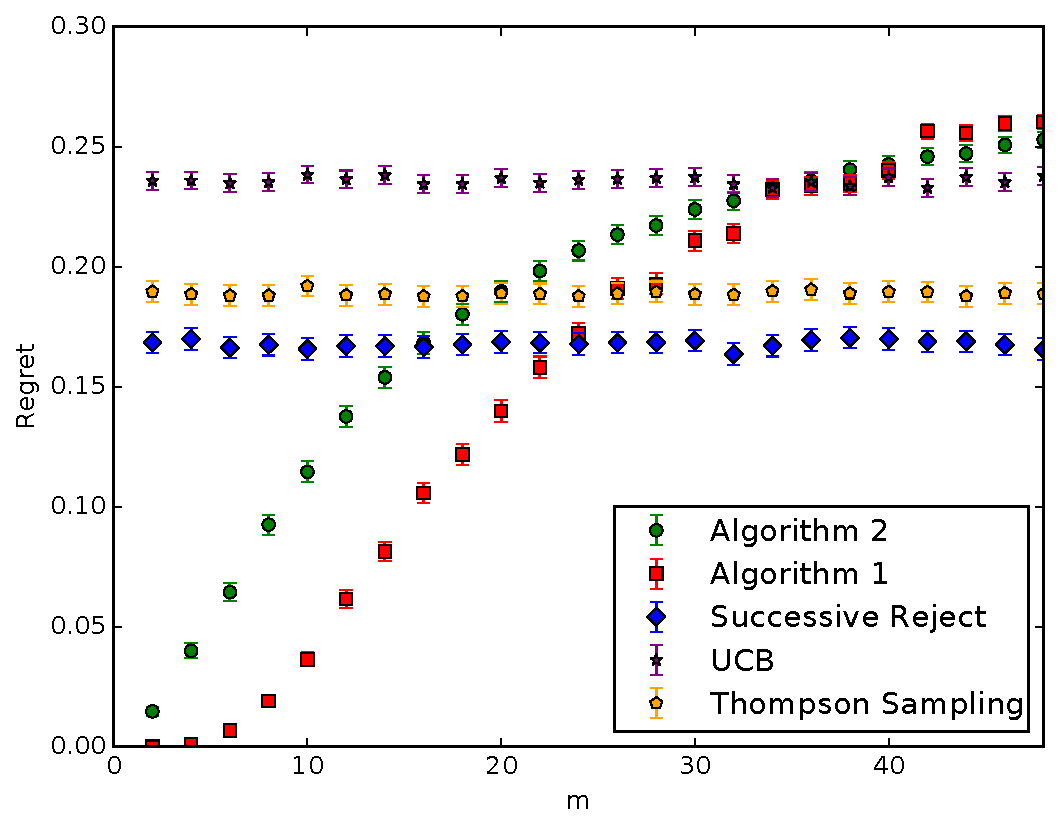
\includegraphics[width=\textwidth]{experiment1_20161020_1247.pdf}
    		\caption{Simple regret vs $m(\boldsymbol{q})$ for fixed horizon $T=400$ and number of variables $N = 50$}
        \label{fig:simple_vs_m}
    \end{subfigure}\hfill
    \begin{subfigure}[t]{0.3\textwidth}
    		\centering
        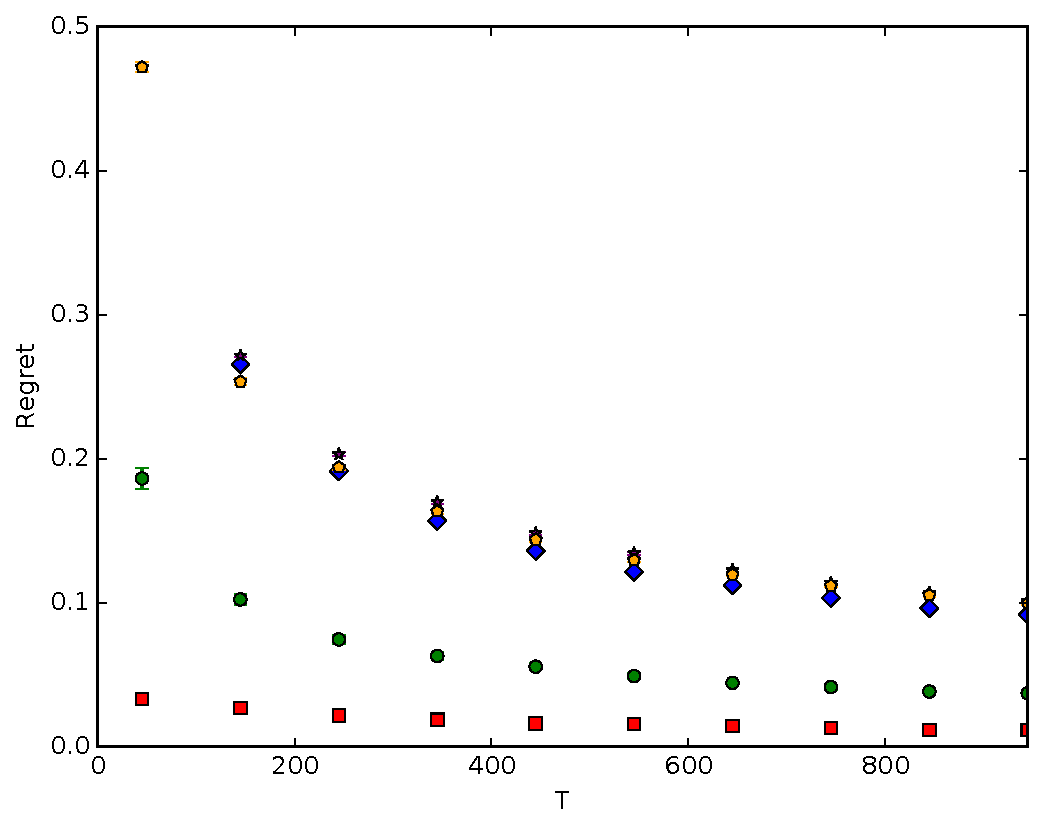
\includegraphics[width=\textwidth]{experiment2_20161020_1249.pdf}
    		\caption{Simple regret vs horizon, $T$, with $N = 50$, $m=2$ and $\epsilon = \sqrt{\frac{N}{8T}}$}
        \label{fig:simple_vs_T_vary_epsilon}
    \end{subfigure}\hfill
    \begin{subfigure}[t]{0.3\textwidth}
    		\centering
    		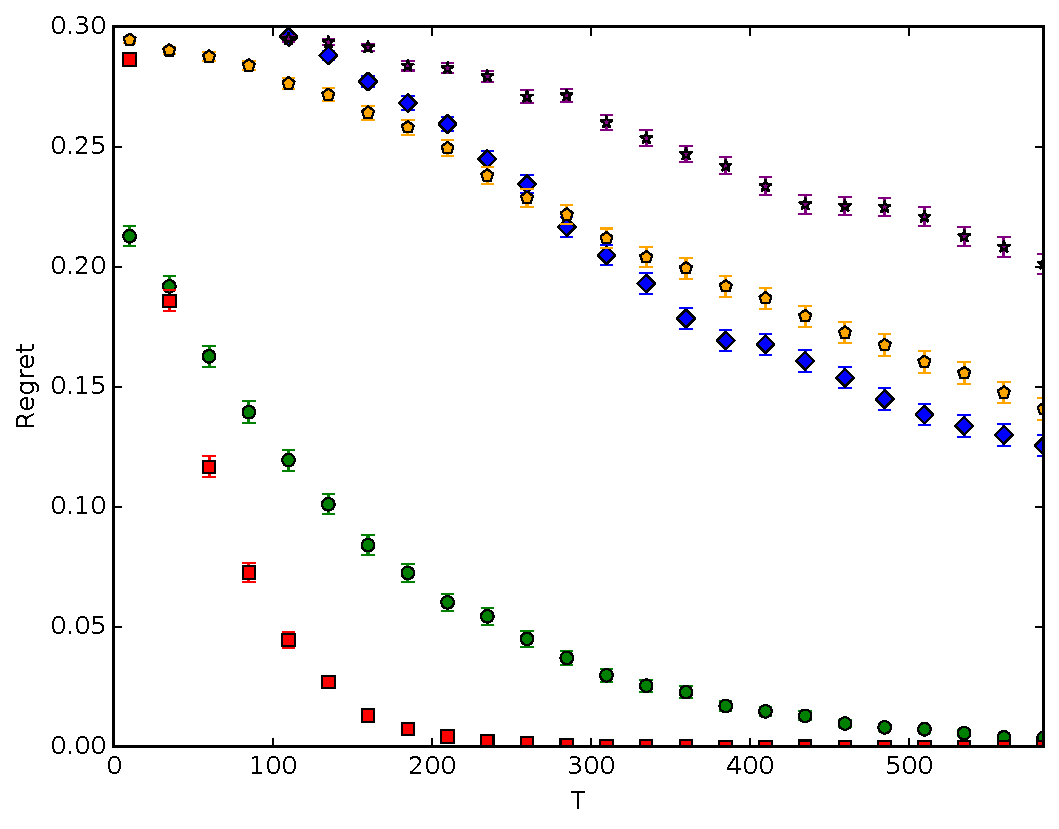
\includegraphics[width=\textwidth]{experiment3_20161020_1252.pdf}
    		\caption{Simple regret vs horizon, $T$, with $N = 50$, $m=2$ and fixed $\epsilon = .3$}
    		\label{fig:simple_vs_T}
    \end{subfigure}
    \caption{Experimental results}
    \label{fig:experiments}
\end{figure}

Figure \ref{fig:simple_vs_T_vary_epsilon} demonstrates the performance of the algorithms in the worst case environment for standard bandits, where the gap between the optimal and sub-optimal arms, $\smash{\epsilon = \sqrt{N/(8T)}}$ , is just too small to be learned. This gap is learn-able by the causal algorithms, for which the worst case $\epsilon$ depends on $m \ll N$. In Figure \ref{fig:simple_vs_T} we fix $N$ and $\epsilon$ and observe that, for sufficiently large $T$, the regret decays exponentially. The decay constant is larger for the causal algorithms as they have observed a greater effective number of samples for a given $T$. 

For the parallel bandit problem, the regression estimator used in the specific algorithm outperforms the truncated importance weighted estimator in the more general algorithm, despite the fact the specific algorithm must estimate $\boldsymbol{q}$ from the data. 
This is an interesting phenomenon that has been noted before in off-policy evaluation where the regression (and not the importance weighted) estimator is known to be mini-max optimal asymptotically \citep{LMS14}.


\begin{figure}[H]
	\centering    
          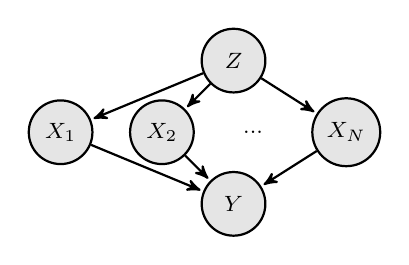
\begin{tikzpicture}[->,>=stealth',shorten >=1pt,auto,node distance=.45cm,
  thick,main node/.style={observed}, hidden/.style={empty},background rectangle/.style={fill=olive!45}]
%every node/.style={scale=0.6}
 %nodes
\node[main node](1){$X_{1}$};
\node[main node, right=of 1](2){$X_{2}$};
\node[hidden, right=of 2](3){$...$};
\node[main node, right=of 3](4){$X_{N}$};
\node[main node, below right=of 2](5){$Y$};
\node[main node, above right=of 2](6){$Z$};
 \path[every node/.style={font=\tiny}]
    (1) edge (5)
    	(2) edge (5)
    (4) edge (5)
    (6) edge (1) edge (2) edge (4);
\end{tikzpicture}
        \caption{Confounded graph}
        \label{fig:parallel_confounded} 
\end{figure}


We now compare the general algorithm with a range of standard bandit algorithms on the confounded graph in Figure \ref{fig:parallel_confounded}. All the variables are binary and the action space consists of the set of single variable interventions plus the do nothing action, 

\eq{
\calA = \set{\set{do(X_i = j)} \cup \set{do(Z = j)} \cup \set{do()}: 1\leq i \leq N,\; j \in \set{0,1}}
} 

We choose this setting because it generalises the parallel bandit, while simultaneously being sufficiently simple that we can compute the exact reward and interventional distributions for large $N$ (in general inference in graphical models is exponential in $N$). As before, we show the average regret over 10,000 simulations with error bars showing three standard errors. 

In Figure \ref{fig:simple_vs_m_general} we fix $N$ and $T$ and $P(Z=1) = .4$. For some $2 \leq N_1 \leq N$ we define 
\eq{
P(X_i = 1|Z = 0) &= \begin{cases} 0 & \text{ if } i \in \set{1,...N_1} \\ .4 & \text{ otherwise } \end{cases}\\
P(X_i = 1|Z = 1) &= \begin{cases} 0 & \text{ if } i \in \set{1,...N_1} \\ .65 & \text{ otherwise } \end{cases}
}
As in the parallel bandit case, we let $Y$ depend only on $X_1$, $P(Y|do(X_1=1)) = \frac{1}{2} + \epsilon$ and $P(Y|do(X_1=0)) = \frac{1}{2}-\epsilon'$, where $\epsilon' = \epsilon P(X_1=1) / P(X_1=0)$. The value of $N_1$ determines $m$ and ranges between $2$ and $N$. The values for the CPD's have been chosen such that the reward distribution is independent of $m$ and so that we can analytically calculate $\eta*$. This allows us to just show the dependence on $m$, removing the noise associated with different models selecting values for $\eta*$ with the same $m$ (and also worst case performance), but different performance for a given reward distribution. 

In Figure \ref{fig:simple_vs_T_general} we fix the model and number of variables, $N$, and vary the horizon $T$. $P(Z)$ and $P(X|Z)$ are the same as for the previous experiment.  
In Figure \ref{fig:simple_vs_T_misspecified} we additionally show the performance of Algorithm 1, but exclude actions on $Z$ from the set of allowable actions to demonstrate that Algorithm 1 can fail in the presence of a confounding variable, which occurs because it incorrectly assumes that $P(Y|do(X)) = P(Y|X)$. 
We let $P(Z) = .6$, $P(Y|\boldsymbol{X}) = X_7 \oplus X_N$ and $P(X|Z)$ be given by:

\eq{
P(X_i = 1|Z = 0) &= 
\begin{cases} 
.166 & \text{ if } i \in \set{1,..., 6} \\
.2 & \text{ if } i = 7 \\
.7 & \text { otherwise} 
 \end{cases}\\
 P(X_i = 1|Z = 1) &= 
\begin{cases} 
.166 & \text{ if } i \in \set{1,..., 6} \\
.8 & \text{ if } i = 7 \\
.3 & \text { otherwise} 
 \end{cases}\\
}

In this setting $X_7$ tends to agree with $Z$ and $X_N$ tends to disagree. It is sub-optimal to act on either $X_7$ or $X_N$, while all other actions are optimal. The first group of $X$ variables with $i \leq 6$ will be identified by the parallel bandit as the most unbalanced ones and played explicitly. All remaining variables are likely to be identified as balanced and estimated from observational estimates. The CPD values have been chosen to demonstrate the worst case outcome, where the bias in the estimates leads Algorithm 1 to asymptotically select a sub-optimal action.

\begin{figure}[H]
    \begin{subfigure}[t]{0.3\textwidth}
		\centering    
    		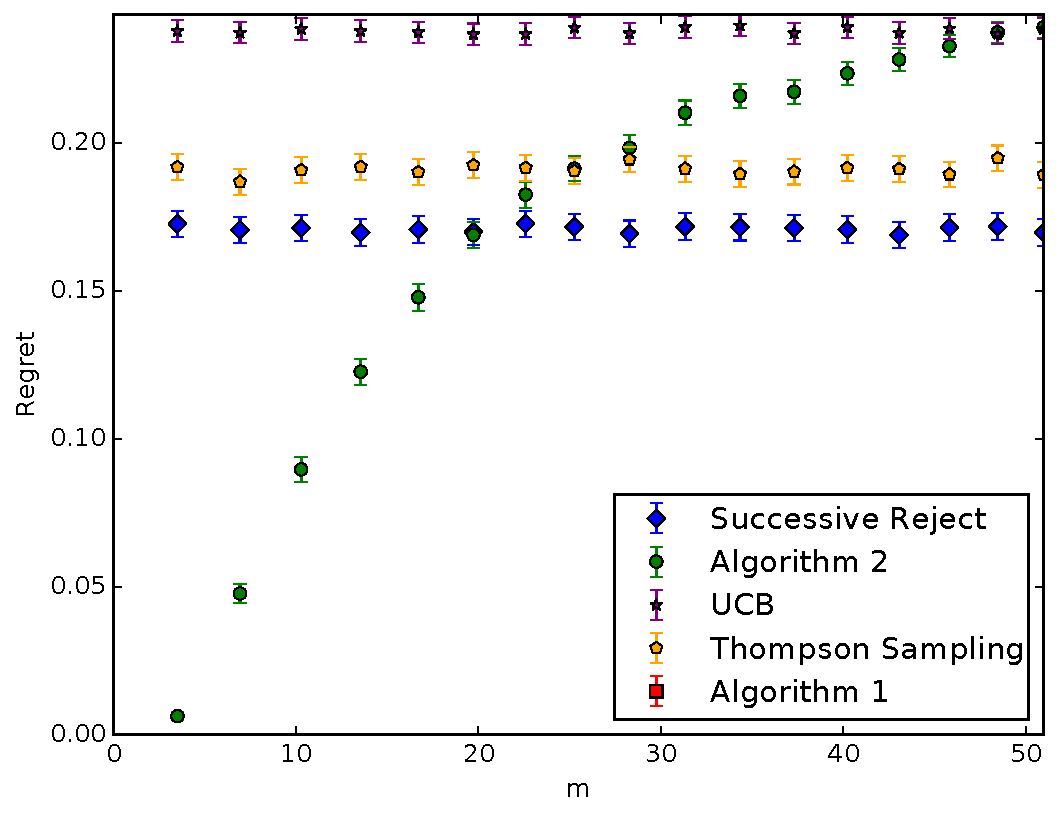
\includegraphics[width=\textwidth]{experiment4_20161023_2120.pdf}
    		\caption{Simple regret vs $m(\eta*)$ for fixed horizon $T=400$ and number of variables $N = 50$}
        \label{fig:simple_vs_m_general}
    \end{subfigure}\hfill
    \begin{subfigure}[t]{0.3\textwidth}
    		\centering
        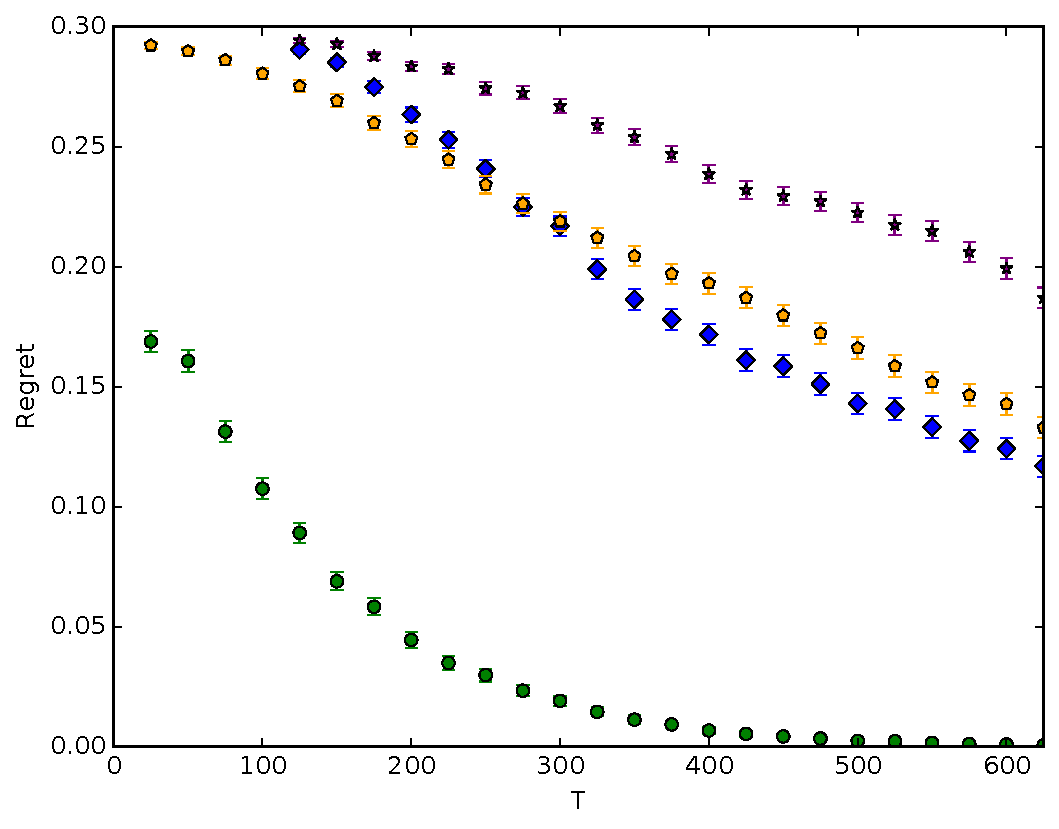
\includegraphics[width=\textwidth]{experiment7_20161020_1257.pdf}
    		\caption{Simple regret vs horizon, $T$, with $N = 50$ and $m(\eta*)=3.1$ }
        \label{fig:simple_vs_T_general}
    \end{subfigure}\hfill
    \begin{subfigure}[t]{0.3\textwidth}
    		\centering
    		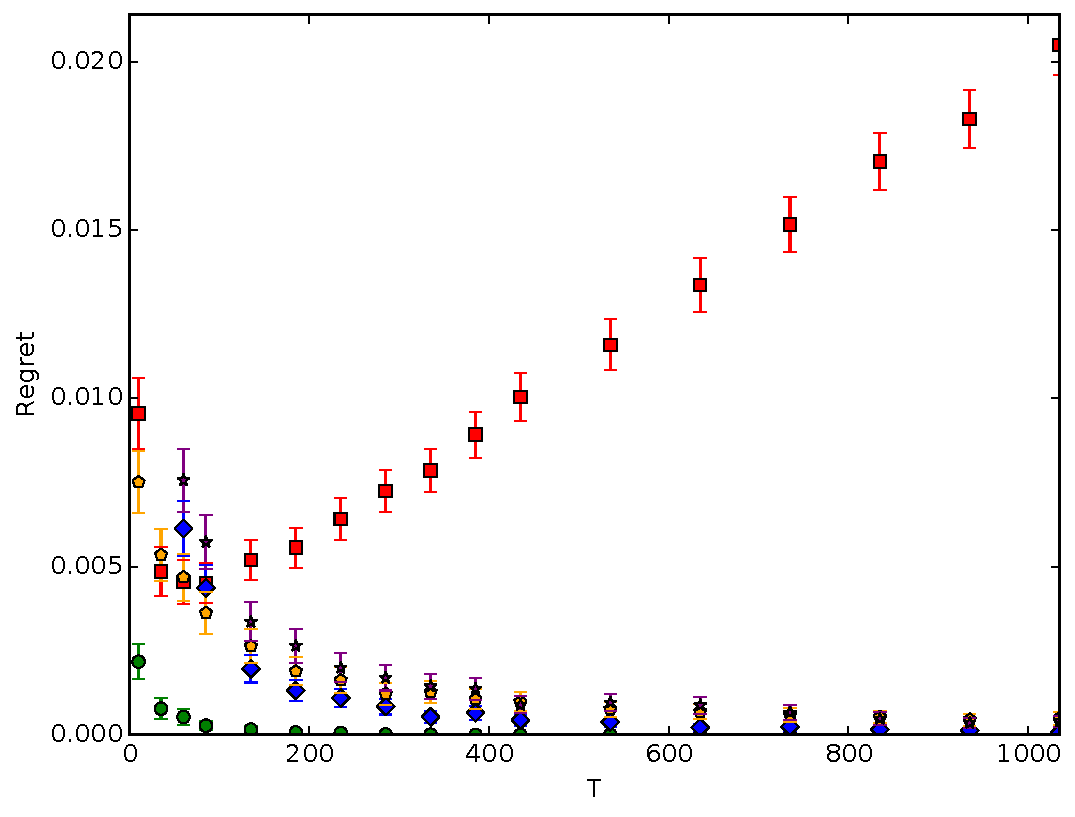
\includegraphics[width=\textwidth]{experiment5_20161023_2118.pdf}
    		\caption{Simple regret vs horizon, $T$, with $N = 21$, $m(\eta*)=4.3$ with no actions setting $Z$}
    		\label{fig:simple_vs_T_misspecified}
    \end{subfigure}
    \caption{Experimental results on the confounded graph}
    \label{fig:experiments_confounded}
\end{figure}

\subsection{Discussion \& Future work}
\label{sec:causal_bandit_discussion}
Algorithm~\ref{alg:general} for general causal bandit problems 
estimates the reward for all allowable interventions $a \in \calA$ over $T$ rounds by sampling and applying interventions from a distribution $\eta$.
Theorem~\ref{thm:general} shows that this algorithm has (up to log factors) simple regret that is $\smash{\mathcal O(\sqrt{m(\eta)/T)}}$ where 
the parameter $m(\eta)$ measures the difficulty of learning the causal model and is always less than $N$.
The value of $m(\eta)$ is a uniform bound on the variance of the reward estimators $\hat{\mu}_a$ and, intuitively, problems where all variables' values in the causal model ``occur naturally'' when interventions are sampled from $\eta$ will have low values of $m(\eta)$.

The main practical drawback of Algorithm~\ref{alg:general} is that both the estimator $\hat{\mu}_a$ and the optimal sampling distribution $\eta^*$ (\ie, the one that minimises $m(\eta)$) require knowledge of the conditional distributions $\Pn{a}{\parents{Y}}$ for all $a \in \calA$. In contrast, in the special case of parallel bandits, Algorithm~\ref{alg:simple} uses the $do()$ action to effectively estimate $m(\eta)$ and the rewards then re-samples the interventions with variances that are not bound by $\hat{m}(\eta)$.
Despite these extra estimates, Theorem~\ref{thm:lower} shows that this approach is optimal (up to log factors).Finding an algorithm that only requires the causal graph and lower bounds for its simple regret in the general case is left as future work.


\paragraph{Making Better Use of the Reward Signal}
Existing algorithms for best arm identification are based on ``successive rejection'' (SR) of arms based on UCB-like bounds on their rewards~\citep{Even-Dar2002}. In contrast, our algorithms completely ignore the reward signal when developing their arm sampling policies and only use the rewards when estimating $\hat{\mu}_a$. Incorporating the reward signal into our sampling techniques or designing more adaptive reward estimators that focus on high reward interventions is an obvious next step. This would likely improve the poor performance of our causal algorithm relative to the successive rejects algorithm for large $m$, as seen in Figure~\ref{fig:simple_vs_m}.

For the parallel bandit the required modifications should be quite straightforward. The idea would be to adapt the algorithm to essentially use successive elimination in the second phase so arms are eliminated as soon as they are provably no longer optimal with high probability. In the general case a similar modification is also possible by dividing the budget $T$ into phases and optimising the sampling distribution $\eta$, eliminating arms when their confidence intervals are no longer overlapping. Note that these modifications will not improve the mini-max regret, which at least for the parallel bandit is already optimal. For this reason we prefer to emphasise the main point that causal structure should be exploited when available. Another observation is that Algorithm \ref{alg:general} is actually using a fixed design, which in some cases may be preferred to a sequential design for logistical reasons. This is not possible for Algorithm \ref{alg:simple}, since the $\vec{q}$ vector is unknown.


\paragraph{Cumulative Regret}
Although we have focused on simple regret in our analysis, it would also be natural to consider the cumulative regret. In the case of the parallel bandit problem we can slightly modify the analysis from \citep{wu2015online} on bandits with side information 
to get near-optimal cumulative regret guarantees. They consider a finite-armed bandit model with side information where in reach round the learner chooses an action and receives a Gaussian reward signal for all actions, but with a known variance that depends on the chosen action. In this way the learner can gain information about actions it does not take with varying levels of accuracy. The reduction follows by substituting the importance weighted estimators in place of the Gaussian reward. In the case that $\vec{q}$ is known this would lead to a known variance and the only (insignificant) difference is the Bernoulli noise model. In the parallel bandit case we believe this would lead to near-optimal cumulative regret,
at least asymptotically. 

%Their model assumes the rewards for all arms $a$ are Gaussian with mean $\mu_a$ and variance $\sigma^2_{ab}$ and that playing an arm $a$ will reveal a side observation $Y_{ab}$ of the reward for all arms $b$ distributed with mean $\mu_b$ and variance $\sigma^2_{ab}$.
%We can build a similar dependence structure with variances for a Bernoulli reward variable that is derived from the $\vec{q}$ vector of probabilities.
%\todom{Check this!}
%Even though the original results are for Gaussian rewards we believe the analysis will go through largely unchanged.

The parallel bandit problem can also be viewed as an instance of a time varying graph feedback problem \citep{Alon2015,Kocak2014}, where at each time step the feedback graph $G_t$ is selected stochastically, dependent on $\boldsymbol{q}$, and revealed after an action has been chosen. The feedback graph is distinct from the causal graph. A link $A \rightarrow B$ in $G_t$ indicates that selecting the action $A$ reveals the reward for action $B$. For this parallel bandit problem, $G_t$ will always be a star graph with the action $do()$ connected to half the remaining actions. However, \citet{Alon2015,Kocak2014} give adversarial algorithms, which when applied to the parallel bandit problem obtain the standard bandit regret. A malicious adversary can select the same graph each time, such that the rewards for half the arms are never revealed by the informative action. This is equivalent to a nominally stochastic selection of feedback graph where $\boldsymbol{q} = \boldsymbol{0}$. 

\cite{Lelarge2012} consider a stochastic version of the graph feedback problem, but with a fixed graph available to the algorithm before it must select an action. In addition, their algorithm is not optimal for all graph structures and fails, in particular, to provide improvements for star like graphs as in our case. \cite{Buccapatnam2014} improve the dependence of the algorithm on the graph structure but still assume the graph is fixed and available to the algorithm before the action is selected. 



\paragraph{Causal Models with Non-Observable Variables}
If we assume knowledge of the conditional \textit{interventional} distributions $\Pn{a}{\parents{Y}}$ our analysis applies unchanged to the case of causal models with 
non-observable variables. Some of the interventional distributions may be non-identifiable meaning we can not obtain prior estimates for $\Pn{a}{\parents{Y}}$ from 
even an infinite amount of observational data. Even if all variables are observable and the graph is known, if the conditional distributions are unknown, then Algorithm
\ref{alg:general} cannot be used. Estimating these quantities while simultaneously minimising the simple regret is an interesting and challenging open problem.

% For example, if we had access to a data set of \textit{experiments} in which the reward variable $Y$ was not available from which to build estimates of $P_a$.
% In this case, some conditional distributions may be non-identifiable. 
% The corresponding actions can be immediately added to the set $A$ prior to collecting any data. 
% We can then use the same algorithm as in the case where there are no latent variables, except that we will have to use the more general do-calculus rather than simply adjusting for the parents to write the expression for each action in terms of observational data.
% Combining our estimation techniques with insights from \citet{Bareinboim2015} for handling unobserved confounders would be worth investigation.


% More generally, assuming causal structure creates more complex types of side information, such as that shown in equation \ref{eq:estimation_transfer}. In this case, selecting one action does not fully reveal an alternate action but provides some information towards an estimate. The quality of the estimate notably depends not only on the number of times that action was selected. For example, to get a good estimate for $X_1 = 1$ by intervening on $X_2$ requires us to sample both $X_2=0$ and $X_2=1$, in proportions dependent on $q_2$. This more complex side information does not fit within the graph feedback framework.


\paragraph{Partially or Completely Unknown Causal Graph}
A much more difficult generalisation would be to consider causal bandit problems where the causal graph is completely unknown or known to be a member of class of models.
The latter case arises naturally if we assume free access to a large observational data set, from which the Markov equivalence class can be found via causal discovery techniques. 
Work on the problem of selecting experiments to discover the correct causal graph from within a Markov equivalence class~\cite{Eberhardt2005,eberhardt2010causal,hauser2014two,Hu2014} could potentially be incorporated into a causal bandit algorithm.
In particular, \citet{Hu2014} show that only $\bigo{\log \log n}$ multi-variable interventions are required on average to recover a causal graph over $n$ variables once purely observational data is used to recover the ``essential graph''.
Simultaneously learning a completely unknown causal model while estimating the rewards of interventions without a large observational data set would be much more challenging.

\subsection{Proofs}
\subsubsection{Proof of Theorem \ref{thm:uq-simple}}\label{sec:thm:uq-simple}


Assume without loss of generality that $q_1 \leq q_2 \leq \ldots \leq q_N \leq 1/2$. The assumption is non-restrictive since all variables
are independent and permutations of the variables can be pushed to the reward function. 

The proof of Theorem \ref{thm:uq-simple} requires some lemmas. \

\begin{lemma}\label{lem:conc1}
Let $i \in \set{1,\ldots, N}$ and $\delta > 0$. Then
\eq{
\P{\left|\hat q_i - q_i\right| \geq \sqrt{\frac{6q_i}{T} \log \frac{2}{\delta}}} \leq \delta\,.
}
\end{lemma}

\begin{proof}
By definition, $\hat{q}_i = \frac{2}{T}\sum_{t=1}^{T/2}X_{t,i}$, where $X_{t,i} \sim Bernoulli(q_i)$. Therefore from the Chernoff bound (see equation 6 in \cite{hagerup1990guided}),

\eq{
\P{\left|\hat q_i - q_i\right| \geq \epsilon} \leq 2e^{-\frac{T\epsilon^2}{6q_i}}
}

Letting $\delta = 2e^{-\frac{T\epsilon^2}{6q_i}}$ and solving for $\epsilon$ completes the proof.

\end{proof}

\begin{lemma}\label{lem:m_est}

Let $\delta \in (0,1)$ and assume $T \geq 48m \log\frac{2N}{\delta}$. Then
\eq{
\P{2m(\vec{q}) / 3 \leq m(\vec{\hat q}) \leq 2m(\vec{q})} \geq 1 - \delta\,.
}
\end{lemma}

\begin{proof}
Let $F$ be the event that there exists and $1 \leq i \leq N$ for which
\eq{
\left|\hat q_i - q_i\right| \geq \sqrt{\frac{6q_i}{T} \log \frac{2N}{\delta}}\,.
}
Then by the union bound and Lemma \ref{lem:conc1} we have $\P{F} \leq \delta$. The result will be completed by showing that
when $F$ does not hold we have $2m(\vec{q})/3 \leq m(\vec{\hat q}) \leq 2m(\vec{q})$.
From the definition of $m(\vec{q})$ and our assumption on $\vec{q}$ we have for $i > m(\vec{q})$ that $q_i \geq q_m \geq 1/m(\vec{q})$ and so by Lemma \ref{lem:conc1} we have
\eq{
\frac{3}{4} 
&\geq \frac{1}{2} + \sqrt{\frac{3}{T} \log \frac{2N}{\delta}} 
\geq q_i + \sqrt{\frac{6q_i}{T} \log \frac{2N}{\delta}} 
\geq \hat q_i \\
&\geq q_i - \sqrt{\frac{6q_i}{T} \log \frac{2N}{\delta}}
\geq q_i - \sqrt{\frac{q_i}{8m(\vec{q})}}
\geq \frac{1}{2m(\vec{q})}\,.
}
Therefore by the pigeonhole principle we have $m(\vec{\hat q}) \leq 2m(\vec{q})$.
For the other direction we proceed in a similar fashion. Since the failure event $F$ does not hold we have for $i \leq m(\vec{q})$ that
\eq{
\hat q_i 
\leq q_i + \sqrt{\frac{6q_i}{T} \log\frac{2N}{\delta}} 
\leq \frac{1}{m(\vec{q})} \left(1 + \sqrt{\frac{1}{8}}\right)
\leq \frac{3}{2m(\vec{q})}\,.
}
Therefore $m(\vec{\hat q}) \geq 2m(\vec{q}) / 3$ as required. 
\end{proof}

\begin{proof}[Proof of Theorem \ref{thm:uq-simple}]
Recall that $A = \set{a \in \actions : \hat p_a \leq 1/m(\vec{\hat q})}$. Then,
for $a \in A$, the algorithm estimates $\mu_a$ from $T_A \doteq T/(2m(\vec{\hat q}))$ samples. From lemma \ref{lem:m_est}, $T_A  \geq T/(4m(\vec{q}))$ with probability $(1-\delta)$. Let $H$ be the event $T_A < T/(4m(\vec{q}))$ and $G$ be the event $\exists a \in A : |\mu_a - \hat \mu_a| \geq \sqrt{\frac{2m(\vec{q})}{T} \log\frac{2N}{\delta}}$

\eq{
\P{G} \leq \P{H} + \P{G|\neg H} \leq \delta + \P{G|\neg H}
}

Via Hoeffding's inequality and the union bound, 

\eq{
\P{G|\neg H}&\doteq \P{\exists a \in A : |\mu_a - \hat \mu_a| \geq \sqrt{\frac{2m(\vec{q})}{T} \log\frac{2N}{\delta}},\text{ given }T_A \geq T/(4m(\vec{q}))} \leq \delta\\
 \implies  \P{G} & \doteq \P{\exists a \in A : |\mu_a - \hat \mu_a| \geq \sqrt{\frac{2m(\vec{q})}{T} \log\frac{2N}{\delta}}} \leq 2\delta\,.
}
For arms not in $A$,

\eq{
\hat p_a = & \frac{2}{T} \sum_{t=1}^{T/2} \ind{X_i = j} \geq 1/m(\vec{\hat q}), \; \text {by definition of not being in $A$}\\
 \geq & \frac{1}{2m(\vec{q})},\; \text{ with probability } 1-\delta \\
\implies  T_a \doteq & \sum_{t=1}^{T/2} \ind{X_i = j} \geq  \frac{T}{4m(\vec{q})},\; \text{ with probability } 1-\delta
}

Again applying Hoeffding's and the union bound

\eq{
\P{\exists a \notin A:  \left|\hat \mu_a - \mu_a\right| \geq \sqrt{\frac{2m(\vec{q})}{T} \log \frac{2N}{\delta}}} \leq 2\delta
}


Therefore, combining this result with the bound for arms $a \in A$, we have with probability at least $1 - 4\delta$ that,
\eq{
(\forall a \in \actions) \qquad |\hat \mu_a - \mu_a| \leq \sqrt{\frac{2m(\vec{q})}{T} \log \frac{2N}{\delta}} \doteq \epsilon\,.
}
If this occurs, then 
\eq{
\mu_{\hat a^*_T} \geq \hat \mu_{\hat a^*_T} - \epsilon \geq \hat \mu_{a^*} - \epsilon \geq \mu_{a^*} - 2\epsilon\,.
}
Therefore
\eq{
\mu^* - \EE[\mu_{\hat a^*_T}] 
& \leq 4\delta + \epsilon\\
& \leq \frac{8m(\vec{q})}{T} + \sqrt{\frac{2m(\vec{q})}{T} \log \frac{NT}{m(\vec{q})}},\; \text{ letting } \delta = \frac{2m(\vec{q})}{T}\\
& \leq \sqrt{\frac{20m(\vec{q})}{T} \log \frac{NT}{m(\vec{q})}},\; \text{ via Jenson's Inequality}
}
which completes the result.
\end{proof}

%%%%%%%%%%%%%%%%%%%%%%%%%%%%%%%%%%%%%%%%%%%%
% LOWER BOUND
%%%%%%%%%%%%%%%%%%%%%%%%%%%%%%%%%%%%%%%%%%%%
\subsubsection{Proof of Theorem \ref{thm:lower}}\label{sec:thm:lower}

We follow a relatively standard path by choosing multiple environments that have different optimal arms, but which cannot all be statistically
separated in $T$ rounds.
Assume without loss of generality that $q_1 \leq q_2 \leq \ldots \leq q_N \leq 1/2$.
For each $i$ define reward function $r_i$ by
\eq{
r_0(\boldsymbol{X}) &= \frac{1}{2} &
r_i(\boldsymbol{X}) &= \begin{cases}
\frac{1}{2} + \epsilon & \text{if } X_i = 1 \\
\frac{1}{2} & \text{otherwise}\,,
\end{cases}
}
where $1/4 \geq \epsilon > 0$ is some constant to be chosen later.
We abbreviate $R_{T,i}$ to be the expected simple regret incurred when interacting with the
environment determined by $\boldsymbol{q}$ and $r_i$. Let $\operatorname{P}_i$ be the corresponding measure
on all observations over all $T$ rounds and $\EE_i$ the expectation with respect to $\operatorname{P}_i$. By Lemma 2.6 by \citet{Tsy08} we have
\eq{
\Prz{\hat a^*_T = a^*} + \Pri{\hat a^*_T \neq a^*} \geq \exp\left(-\KL(\operatorname{P}_0, \operatorname{P}_i)\right)\,,
}
where $\KL(\Ps_0, \Ps_i)$ is the KL divergence between measures $\operatorname{P}_0$ and $\operatorname{P}_i$.
Let $T_i(T) = \sum_{t=1}^T \ind{a_t = do(X_i = 1)}$ be the total number of times the learner intervenes on variable $i$ by setting it to $1$.
Then for $i \leq m$ we have $q_i \leq 1/m$ and the KL divergence between $\Ps_0$ and $\Ps_i$ may be bounded using the telescoping property (chain rule) and
by bounding the local KL divergence by the $\chi$-squared distance as by \citet{Auer1995}. This leads to 
\eq{
\KL(\Ps_0, \Ps_i) 
&\leq 6\epsilon^2 \EE_0\left[\sum_{t=1}^T \ind{X_{t,i} = 1}\right] 
\leq 6\epsilon^2 \left(\EE_0 T_i(T) + q_i T\right) 
\leq 6\epsilon^2 \left(\EE_0 T_i(T) + \frac{T}{m}\right)\,.
}
Define set $A = \set{i \leq m : \EE_0 T_i(T) \leq 2T / m}$.
Then for $i \in A$ and choosing $\epsilon = \min\set{1/4, \sqrt{m/(18T)}}$ we have
\eq{
\KL(\Ps_0, \Ps_i) \leq \frac{18T\epsilon^2}{m} = 1\,. 
}
Now $\sum_{i=1}^m \EE_0 T_i(T) \leq T$, which implies that $|A| \geq m/2$.
Therefore
\eq{
\sum_{i \in A} \Pri{\hat a^*_T \neq a} 
\geq \sum_{i \in A} \exp\left(-\KL(\Ps_0, \Ps_i)\right) - 1
\geq \frac{|A|}{e} - 1 
\geq \frac{m}{2e} - 1\,.
}
Therefore there exists an $i \in A$ such that
$\Pri{\hat a^*_T \neq a^*} \geq \frac{\frac{m}{2e} - 1}{m}$. 
Therefore if $\epsilon < 1/4$ we have
\eq{
R_{T,i} \geq \frac{1}{2} \Pn{i}{\hat a^*_T \neq a^*} \epsilon \geq \frac{\frac{m}{2e} - 1}{2m} \sqrt{\frac{m}{18T}}\,.
}
Otherwise $m \geq 18T$ so $\sqrt{m/T} = \Omega(1)$ and
\eq{
R_{T,i} \geq \frac{1}{2} \Pn{i}{\hat a^*_T \neq a^*} \epsilon \geq \frac{1}{4} \frac{\frac{m}{2e} - 1}{2m} \in \Omega(1) 
}
as required.

%%%%%%%%%%%%%%%%%%%%%%%%%%%%%%%%%%%%%%%%%%%%
% GENERAL-GRAPH UPPER BOUND
%%%%%%%%%%%%%%%%%%%%%%%%%%%%%%%%%%%%%%%%%%%%
\subsubsection{Proof of Theorem \ref{thm:general}}\label{sec:thm:general}

\begin{proof}
First note that $X_t, Y_t$ are sampled from $\operatorname{Q}$.
We define $Z_a(X_t) = Y_t R_a(X_t)\ind{R_a(X_t)\leq B_a}$ and abbreviate $Z_{at} = Z_a(X_t)$, $R_{at} = R_a(X_t)$ and $\Pn{a}{.} = \Pns{a}{.}$.
By definition we have $|Z_{at}| \leq B_a$ and 
\eq{
\Var_Q[Z_{at}] 
\leq \EE_Q[Z_{at}^2] 
\leq \EE_Q[R_{at}^2]
= \EEa[R_{at}]
= \EEa\left[\frac{\Pns{a}{\parents{Y}(X)}}{\Q{\parents{Y}(X)}}\right] 
\leq m(\eta)\,.
}
Checking the expectation we have
\eq{
\EE_Q[Z_{at}] 
= \EEa \left[Y \ind{R_{at} \leq B_a}\right] 
= \EEa Y - \EEa \left[Y\ind{R_{at} > B_a}\right] 
= \mu_a - \beta_a\,,
}
where 
\eq{
0 \leq \beta_a = \EEa[Y \ind{R_{at} > B_a}] \leq \Pns{a}{R_{at} > B_a}
}
is the negative bias. 
The bias may be bounded in terms of $m(\eta)$ via an application of Markov's inequality.
\eq{
\beta_a \leq \Pns{a}{R_{at} > B_a} \leq \frac{\EEa[R_{at}]}{B_a} \leq \frac{m(\eta)}{B_a}\,.
}
Let $\epsilon_a > 0$ be given by
\eq{
\epsilon_a = \sqrt{\frac{2m(\eta)}{T} \log\left(2T|\calA|\right)} + \frac{3B_a}{T} \log\left(2T|\calA|\right)\,.
}
Then by the union bound and Bernstein's inequality 
\eq{
\P{\text{exists } a \in \calA : \left|\hat \mu_a - \EE_Q[Z_{at}]\right| \geq \epsilon_a} 
\leq \sum_{a \in \calA} \P{\left|\hat \mu_a - \EE_Q[Z_{at}]\right| \geq \epsilon_a} \leq \frac{1}{T}\,.
}

Let $I = \hat{a}^*_T$ be the action selected by the algorithm, $a^* = \argmax_{a \in \calA} \mu_a$ be the true optimal action and recall that $\EE_Q[Z_{at}] = \mu_a - \beta_a$. Assuming the above event does not occur we have,

\eq{
\mu_I \geq \hat \mu_I - \epsilon_I  
\geq \hat \mu_{a^*} - \epsilon_I  
\geq \mu^* - \epsilon_{a^*} - \epsilon_I - \beta_{a^*}\,. 
}
By the definition of the truncation
we have
\eq{
\epsilon_a \leq \left(\sqrt{2} + 3\right)\sqrt{\frac{m(\eta)}{T} \log\left(2T|\calA|\right)}
}
and
\eq{
\beta_a \leq \sqrt{\frac{m(\eta)}{T} \log\left(2T|\calA|\right)}\,. 
}
Therefore for $C = \sqrt{2} + 4$ we have
\eq{
\P{\mu_I \geq \mu^* - C \sqrt{\frac{m(\eta)}{T} \log\left(2T|\calA|\right)}} \leq \frac{1}{T}\,.
}
Therefore
\eq{
\mu^* - \EE[\mu_I] \leq C \sqrt{\frac{m(\eta)}{T} \log\left(2T|\calA|\right)} + \frac{1}{T}
}
as required.
\end{proof}

\subsubsection{Relationship between $m(\eta)$ and $m(\boldsymbol{q})$}\label{sec:m-equivelence}

\begin{proposition} In the parallel bandit setting,
$m(\eta^*) \leq 2m(\boldsymbol{q})$.
\end{proposition} 

\begin{proof}

Recall that in the parallel bandit setting,

\eq{
\mathcal{A} = \set{do()} \cup \set{ do(X_i = j) \colon 1 \leq i \leq N \text{ and } j \in \set{0,1}}
}

Let:

\eq {
\eta_a = \ind{\P{X_i = j} < \frac{1}{m(\boldsymbol{q})}}\frac{1}{2m(\boldsymbol{q})} \text { for } a \in do(X_i = j)
}

Let $D =\sum_{a\in do(X_i=j)}\eta_a$. From the definition of $m(\boldsymbol{q})$, 
\eq {
\sum_{a\in do(X_i=j)} \ind{\P{X_i = j} < \frac{1}{m(\boldsymbol{q})}} \leq m(\boldsymbol{q}) \implies D \leq \frac{1}{2}
}
 
Let $\eta_a = \frac{1}{2} + (1-D)$ for $a = do()$ such that $\sum_{a \in \calA}\eta_a = 1$ 

Recall that,

\eq{
m(\eta) &
= \max_a \EEa\left[\frac{\Pn{a}{\parents{Y}(X)}}{\Q{\parents{Y}(X)}}\right]
}

We now show that our choice of $\eta$ ensures $\EEa\left[\frac{\Pn{a}{\parents{Y}(X)}}{\Q{\parents{Y}(X)}}\right] \leq 2m(\boldsymbol{q})$ for all actions $a$.

For the actions $a: \eta_a > 0$, ie $do()$ and $do(X_i = j):\P{X_i=j}<\frac{1}{m(\boldsymbol{q})}$,
\eq{
\EEa\left[\frac{\Pn{a}{X_1...X_N}}{\sum_{b}\eta_b\Pn{b}{X_1...X_N}}\right] \leq \EEa\left[\frac{\Pn{a}{X_1...X_N}}{\eta_a\Pn{a}{X_1...X_N}}\right] = \EEa\left[\frac{1}{\eta_a}\right] \leq 2m(\boldsymbol{q})
}

For the actions $a :\eta_a = 0$, ie $do(X_i=j):\P{X_i=j}\geq\frac{1}{m(\boldsymbol{q})}$,
\eq{
\EEa\left[\frac{\Pn{a}{X_1...X_N}}{\sum_{b}\eta_b\Pn{b}{X_1...X_N}}\right] \leq & \EEa\left[\frac{\ind{X_i=j}\prod_{k\neq i}\P{X_k}}{(1/2+D)\prod_k \P{X_k}}\right] \\=& \EEa\left[\frac{\ind{X_i=j}}{(1/2+D)\P{X_i = j}}\right]
\leq  \EEa\left[\frac{\ind{X_i=j}}{(1/2)(1/m(\boldsymbol{q}))}\right] \leq 2m(\boldsymbol{q})
}

Therefore $m(\eta*) \leq m(\eta) \leq 2m(\boldsymbol{q})$ as required.

\end{proof}
\
%in the parallel bandit setting the $m(\eta)$ given in this section approximately coincides with the $m(\vec{q})$ in Eq.\ \ref{eq:m-simple}.
%Recall in that setting that 
%\eq{
%\actions = \set{do()} \cup \set{do(X_i = j) : 1 \leq i \leq N \text{ and } j \in \set{0,1}}\,.
%}
%For $a = do()$ choose $\eta_a = 1/2$. 
%Let $m = m(\vec{q})$ and note that, by definition, there are at most $m$ pairs $(i,j)$ such that $\P{X_i = j} \leq 1/m$.
%Thus, for $a = do(X_i = j)$ letting $\eta_a \propto \ind{\P{X_i = j} \leq 1/m} / (2m)$ guarantees $\eta_a \ge \frac{1}{2m}$ when $\eta_a \ne 0$.
%It is then easy to check that $m(\eta) \leq 2m$ using an argument like that for Proposition~\ref{pro:m-bound}.


\chapter{More stuff}
%\chapter{List of software programs for causal inference}

\begin{itemize}
\item Pcalg. A library in R that implements ...
\item Tetrad.
\item There has to be a library for the Bayesian trees thing
\item Linear regression (you can do this anywhere)

\end{itemize}


Notorious paper Automated Inferences of Criminality using Face Images. - What possible actions could we take? Ban people with most risky 'face types' from critical jobs? But dependent on causal structure, conditioning on the fact that people are in a position to apply for such jobs could reverse the dependency. Ones facial appearance is a readily observable characteristic and there is evidence that people implicity make assumptions on the basis of it. Consider trials where people with 'more criminal' faces got longer sentances for similar crimes. 
%\chapter{Causality \& Interpretability}

%\chapter{Causality \& Fairness}

Generalisation error weights towards regions where density of x is high (it does not care about minorities). 

As machine learning is incorporated into decision making systems that have fundamental impacts on people’s lives, such as in employment, criminal justice, health and financial services, there are increasing concerns over transparency and fairness \cite{WMD, etc}. Realisation that machine learning algorithms can be inherit biases from the data we feed into them and the choices those building them make about what variables to include, etc. 

The European Union’s General Data Protection Regulation \cite{Goodman2016}\todo{check}, due to come into effect in 2018, requires that people can obtain "meaningful information about the logic involved" in an automated decision process . It also stipulates that such decisions should not be based on special categories of personal data (related to ethnicity, political and religions affiliation or sexuality) unless there "suitable measures" to safeguard individual interests. A key concern is discrimination against disadvantaged groups. 

Discrimination is frequently defined in terms of either disparate treatment- treating otherwise similar individuals differently on the basis of a protected attribute such as race or gender, or disparate impact - a process that yields a significant difference in outcome between groups. We consider how the notions of disparate treatment and impact may be formalised and the implications of how this is done for machine learning. We examine the overlap between the motivations for interpretable and causal models, especially with respect to assessing fairness. We look at how causal models mitigate some of the trade-offs between transparency and predictive accuracy and we examine to what extent the causal relationship between an attribute, any protected attributes and the outcome of interest is relevant to assessing the impact on fairness of its inclusion in a machine learning model.

The lack of part-time work in tech could be argued to constitute indirect discrimination against women. 
A fear that advertising themselves as supporting flexible working options would attract candidates who lacked drive and ambition.
Cultural bias that favours those driven by monetary ambition against those 


Stability - a non causal model can't tell us about a simple do type operation on  a single variable. 

More broadly, we could draw a model representing the system now that could tell us the result of an intervention on a particular variable (such as setting gender), but the system itself could change (for example with customer preferences). There is a notion that a true causal model should be invariant for all time.

Connection to Simpson's paradox. But what should we condition on? \cite{Romie2010} argue that looking at the department level is the correct viewpoint, since this the point at which hiring decisions were made. However, it could be argued that if one department was attracting a large number of higher quality candidates, the overall size of that department should be higher and that the results seen at Berkeley reflected a bias in favour of male dominated fields. 

Different measures of discrimination - is there a difference between groups (after conditioning on xxx)

To understand how we measure and penalise discrimination, we need to take a step back and ask what are the underlying motivations for fairness?

These differences in underlying cause suggest differences in the approach we should take to remedy them.  

%\section{How does discrimination arise in ML models}
\begin{itemize}
\item bias in historical decisions fed in as training data
\item selection bias in input data, due to deliberate or implicit discrimination such as stop and search
\item deliberate manipulation on the part of the person building the model.
\item The hardest case is historical disadvantage, creating genuine differences between relevant attributes of groups.
\item in bias in the label - what happens if you hire minorities but then your staff treat them badly and as a result they under-perform or leave.  
\end{itemize}

%\section{Defining Descrimination}

Define discrimination in terms of causal effect of protected variable in decision making process. 

\cite{Romei2012} note the relevance of causal inference on discrimination analysis.

“the central question in any employment- discrimination case is whether the employer would have taken the same action had the employee been of 7A recurring problem known as the omitted-variable bias.
A multidisciplinary survey on discrimination analysis 9
a different race (age, sex, religion, national origin etc.) and everything else had been the same” (Carson v. Bethlehem)


Let us mathematically define disparate treatment and disparate impact with respect to a statistical model. We will focus on discrete variables for notational simplicity. Assume we have an outcome of interest $Y$, protected attributes $X$, other covariates $Z$ and a (potentially stochastic) model $f$ that maps $\{x, z\}$ to $y_f \in Y$. For a given model $f$, we have a distribution over the predicted outputs given the inputs, $\P{Y_f|X,Z}$
\vspace{.2cm}
\begin{definition}{Disparate Impact}: A model, $f$, that produces a predictive distribution $\P{Y_f|X,Z}$ has disparate impact if the marginal distribution over the predicted outcome, $Y_f$, depends on a protected attribute.
\eqn{
\exists \set{x_1,x_2} \subset X: \sum_z{\P{Y_f|Z,x_1}\P{Z|x_1}} \neq \sum_z{\P{Y_f|Z,x_2}\P{Z|x_2}}
}
\end{definition}

\begin{definition}{Disparate Treatment}: A model yields disparate treatment if people with identical attributes (excluding protected attributes) are treated differently. 
\eqn{
\P{Y_f|Z,X} \neq \P{Y_f|Z}
}
\end{definition}

Avoiding treating people differently purely on the basis of attributes such as ethnicity and gender and avoiding large differences in important outcomes such as education and income between such groupings both seem like desirable goals. Unfortunately, in general, they conflict with one another, see theorem \ref{thm:disparate_conflict}. Any variable we might wish to avoid discriminating on will be correlated to some other measurable covariate $Z$, making it impossible to avoid both disparate treatment and disparate impact. 
\vspace{.2cm}
\begin{theorem} 
\label{thm:disparate_conflict}
Disparate impact and disparate treatment conflict. Given covariates $Z$ and protected attributes $X$, a model, $f$, cannot be fair with respect to both disparate impact and disparate treatment unless $\P{Z|X} = \P{Z}$.
\begin{proof} Assume $f$ yields no different treatment, then $\P{Y_f|Z,X} = \P{Y_f|Z}$. If we additionally assume no disparate impact, $\sum_z{\P{Y_f|Z}\P{Z|x_1}} = \sum_z{\P{Y_f|Z}\P{Z|x_2}} \;\; \forall \set{x_1,x_2}\subset X$. This holds if and only if $\P{Z|x_1} = \P{Z|x_2} \;\; \forall \set{x_1,x_2} \implies \P{Z|X} = \P{Z}$
\end{proof} 
\end{theorem}  

Further issues.


Disparate treatment, with respect to an observed set of variables $Z$, can be trivially avoided by excluding protected attributes from the training data. 

Problems:
\begin{itemize}
\item Disparate impact and disparate treatment conflict
\item 
\end{itemize}



%\section{Addressing discrimination}

Omitting the protected attribute from the model can increase disparate impact, even if the protected attribute is negatively correlated with the outcome. 


\textit{Disparate treatment} can be trivially avoided by excluding the protected variable from the model. However, this is deeply unsatisfying given the presence of proxy variables and can increase bias (figure \ref{fig:recidivism})

Avoiding \textit{disparate impact} may be be expensive in terms of predictive accuracy and/or require \textit{disparate treatment}. 

\begin{figure}[H]
\caption{Proxies}
\label{fig:recidivism}
	\centering    
          \begin{tikzpicture}[->,>=stealth',shorten >=1pt,auto,node distance=.7cm,
  thick,main node/.style={observedrect}, lt/.style={latentrect} , hidden/.style={empty},background rectangle/.style={fill=olive!45}]
 %nodes
\node[lt](1){Actual priors};
\node[main node, below left=of 1](2){Recorded Priors};
\node[main node, below right=of 1](3){Re-offend};
\node[lt, above left=of 2](4){Stop and Search};
\node[main node, above=of 4](5){Race};
\node[main node, above=of 1](6){Education};
 \path[every node/.style={font=\tiny}]
    (1) edge (2) edge (3)
    (4) edge (2)
    (5) edge (4) edge (6)
    (6) edge (1);
\end{tikzpicture}
\end{figure}


\begin{itemize}
\item There is an additional connection between causality and fairness, that arises when you know that there is a bias in the data and wish to correct for it. In causality, it may be due to selection bias or a confounding variable. In fairness, it may be due to historical disadvantage. In both cases we may have theory that tells us the direction or scale of an effect. IE, we know that race itself has no inherent effect on outcomes such as criminality and education. If you have a data set and a collection of such priors, where the data contradicts these priors due to data bias. How do you best make decisions based on that data? 
\end{itemize}


human decision making can evolve. 

The vagueness inherent in writing laws in natural language allows for them to be re-interpreted. 

There is a lack of diversity in models. (although randomness is in fact inherent in many) - could one leverage this? - you would need an estimate of the probability the model would have assigned each instance to a particular group. 

Only humans can provide the ethics

%\chapter*{Random Questions}
\begin{itemize}
\item Why not use ratios instead of differences in defining causal effects (is it anything to do with statement in Dawid? What about sensitivity of uncertainty in estimators.
\end{itemize}


%\chapter{Causality in Marketing}
Assessing the impact of marketing spend is becoming increasingly important to industry. Billions of dollars \cite{XXX} are spent each year and new marketing channels and opportunities are opening up at an unprecedented rate. 

There are three key approaches to assessing the impact of marketing in the literature. 

The first is to look for correlations across companies on metrics such as how much they spend on marketing \ref{}, how confident they are about their ability to market effectively \ref{} or how important the marketing team is perceived to be within the organisation with indicators of the health of the company such as sales, revenue or market capitalisation. Unfortunately is is very difficult to avoid potential major confounders with this approach. Are businesses large and successful because of their capable marketing teams or can they afford to hire capable marketers because they have sufficient profits available to do so. 

%\section{Attribution}
The second is attribution. The goal in this case is to attribute each sale to a specific (or set of specific) advertisements that the customer was exposed to. This approach is the primary way of measuring the success of digital advertising strategies such as search, display, and online video ads. The most frequent model is last-click attribution. In which the last ad the customer was presented with before they made their purchase is assumed to have caused that sale. A central criticism of attribution is that it is not measuring incremental sales. Each sales is assumed to be a consequence of some form of advertising for those customers who saw (however briefly) some form of advertisement. Of course in reality many of these customers may have made a purchaser regardless of the advertising material to which they were exposed. 

System designed to optimise metrics such as click through or conversion rate can do so either by learning how to change the consumers preferences (by serving them the perfect ad at the ideal time) or by learning who was most likely to buy anyway. It seems likely that much of the improve mt in click through rates due to the application of sophisticated machine learning algorithms is being driven by the latter. Unfortunately, this does nothing for the bottom line of industry (except for those involved in serving ads). 


%\section{Econometric Modelling}
The final key plank businesses apply to estimate how effective their marketing are econometric or mixed media models. These models

In practise these models are typically time series regression models, fitting some measure of sales against marketing spend (by marketing channel, IE TV, radio, search, digital display etc) and other key variables such as pricing, competitor spend and pricing and indicators of the health of the economy and demand for the product in question.

The models may also include non-linear transformation of the marketing inputs to represent saturation and decay of time of effects. They may also consider the interaction between media channels and other business levers such as pricing.  

The objective of these models is to obtain results that are comparable across channels such that the optimal mix of media can be selected. 

The key

\chapter{Conclusion}

%\section{Open questions}
\paragraph{Cycles} - a huge issue. Not covered by Pearl,Rubin etc. 

Places to look, statistical control theory, etc. any interesting papers along these lines?

In the discrete case,
Fung and Crawford (1990) have recently proposed a fast algorithm for constructing an
independence graph from discrete data. We have not tested their procedure as a processor for
the PC algorithm. (COPIED FROM SPRITES)


\bibliographystyle{apalike}% Select the citation style e.g. ieeetr
\bibliography{library}% write the directory to the .bib file
\end{document}




